\documentclass[11pt]{report}
%====================== PACKAGES ======================
%Options: Sonny, Lenny, Glenn, Conny, Rejne, Bjarne, Bjornstrup
\usepackage[Glenn]{fncychap} 
\usepackage{fancyhdr}
\usepackage[final]{pdfpages}
\usepackage{array}
\usepackage{algorithm}
\usepackage{algpseudocode}
\usepackage[english]{babel}
\usepackage[utf8]{inputenc}
%pour gérer les positionnement d'images
\usepackage{float}
\usepackage{placeins}
\usepackage{graphicx}
\usepackage[colorinlistoftodos]{todonotes}
\usepackage{url}
\usepackage{listings}
\lstset{basicstyle=\ttfamily\small,breaklines=true,columns=fullflexible,keepspaces=true}
\usepackage{enumitem}
%pour la mise en page des tableaux
\usepackage{array}
\usepackage{tabularx}
\usepackage{dcolumn,ragged2e}
\usepackage{siunitx}
\usepackage{longtable}
\usepackage{booktabs}   
\usepackage{ltablex}
\newcolumntype{L}{>{\raggedright\arraybackslash}X}
%pour utiliser \floatbarrier
\usepackage{colortbl}
%espacement entre les lignes
\usepackage{setspace}
%modifier la mise en page de l'abstract
\usepackage{abstract}
%police et mise en page (marges) du document
\usepackage[T1]{fontenc}
\usepackage{amsmath}
\usepackage{amsthm}
\usepackage{newtxtext,newtxmath}
\usepackage[top=2cm, bottom=2cm, left=2cm, right=2cm]{geometry}
\usepackage{microtype}
%Pour les galerie d'images
\usepackage{array}
\usepackage{makecell}
\usepackage{multirow}
%\usepackage{subfig}
%\usepackage{graphicx}
%\usepackage{geometry}
\usepackage{titlesec}
\newtheorem{definition}{Definition}
\usepackage{rotating}
\usepackage{pdflscape}
%\usepackage{multirow}
\usepackage{graphicx}
\usepackage{xspace}
\usepackage{wrapfig}
\usepackage[numbers,sort&compress]{natbib}
\usepackage[hypertexnames=false]{hyperref}
\hypersetup{
    colorlinks=true,
    linkcolor=black,
    filecolor=black,      
    urlcolor=black,
    anchorcolor=black,
    citecolor=blue,
}
\usepackage{subcaption}
\usepackage{tablefootnote}
\usepackage[acronym]{glossaries}
\usepackage{xcolor}
\usepackage{caption}
\captionsetup{
    font=small,
    labelfont=bf,
    textfont=it,
    skip=8pt
}
\captionsetup[figure]{position=bottom}
\captionsetup[table]{position=bottom}
\captionsetup[lstlisting]{position=bottom}
\newcommand{\HRule}{\rule{\linewidth}{0.5mm}}

\begin{document}
% Front matter: roman numerals (introduction will be page 1)
\pagenumbering{roman}
\setcounter{page}{1}
%%d'ici aussi
\begin{titlepage}   
    	\begin{minipage}{1\linewidth}
			\centering
			\begin{tabular}{ccc}
				\begin{tabular}{c}
					\\
					
\includegraphics[scale=0.2]{figures/huawei.png}
				\end{tabular}
				&
				\begin{tabular}{c}
					\\
					\text{People's Democratic Republic of Algeria}\\
                    \text{Ministry of Higher Education and Scientific Research}\\
				\end{tabular}
				&
				\begin{tabular}{c}
					\\
					\includegraphics[scale=0.07]{figures/usthb.png}
				\end{tabular}
			\end{tabular}
		\end{minipage}
    
    
       
    \begin{center}
        
        \textbf{University of Science and Technology Houari Boumediene}\\
        \text{Faculty of Computer Science}\\
        \text{Field: Computer Science}\\
        \textbf{Licence Thesis}\\
        \text{Specialization: ISIL}\\
        
        
        
    \end{center}
    \vspace*{0.5 cm}
    \begin{center}
    
    \end{center}
    
    \rule{\linewidth}{0.2 mm}
	{ \LARGE  
	   \begin{center}
	       \textbf{Topic: }\\
	       \textbf{Realization of a Data Center Modern Network Architecture}\\
	       
	   \end{center} 
	   
	\rule{\linewidth}{0.2 mm} \\[1.5 cm]
	}
	
	\begin{minipage}{0.5\textwidth}
		\begin{flushleft} \large
		    \textbf{Supervised by :}\\
		    \text{TETBIRT Ishak}\\
		    \text{GUEBLI Wassila}\\
		    \textbf{Jury Members :}\\
		    \text{GUEBLI Wassila}\\
		    \text{BENCHAIBA Mahfoud}\\
		    
			\end{flushleft}
			\end{minipage}~
		\begin{minipage}{0.4\textwidth}
            
		\begin{flushright} \large
			\textbf{Presented by :} \\
            \text{GRIMES Roumaissa} \\
            \text{ZEGHACHE Aya} \\
            \text{BAKIRI Samy} \\
            \text{BOUSSAID Louai} \\
            	\textbf{Submission date :} \\
            \text{16/05/2026} \\
		\end{flushright}
	\end{minipage}\\[2 cm]
	\begin{center}
	    Projet : ISIL14/2026
	\end{center}
\end{titlepage}
\chapter*{Acknowledgements}
\addcontentsline{toc}{chapter}{Acknowledgements}

We thank ALLAH, the Almighty, for giving us the strength, the will, and above all the courage to accomplish this dissertation.

We express our sincere gratitude to our academic supervisor, Mrs.\ Wassila Guebli, for agreeing to guide and support us throughout this work.

We also extend our deepest thanks to our supervisors at Huawei, Mr.\ Ishak Tetbirt and Mr.\ Ahmed Tarek Lounici, for giving us the opportunity to work on this subject, for their valuable technical guidance, and for their continuous support throughout this project.

We extend our sincere gratitude to the entire Huawei team for their warm welcome, their professionalism, and their constant willingness to help. Their support and shared expertise have been invaluable to the success of this work.

We thank all the professors of the Faculty of Computer Science at the University of Science and Technology Houari Boumediene for the knowledge and skills they have provided us throughout our academic journey.

We express our warmest thanks to all the members of the jury for the honor of evaluating this work.

Finally, we offer a heartfelt thank you to our families for their unwavering support and encouragement throughout this final-year project. Your love and patience have been our greatest strength.

\hypersetup{hidelinks}
\tableofcontents
\chapter*{LIST OF ACRONYMS}
\addcontentsline{toc}{chapter}{LIST OF ACRONYMS}

\begin{longtable}{|p{0.2\textwidth}|p{0.75\textwidth}|}
\hline
\textbf{Acronym} & \textbf{Meaning} \\
\hline
\endfirsthead
\hline
\textbf{Acronym} & \textbf{Meaning} \\
\hline
\endhead
\hline
\multicolumn{2}{|r|}{\textit{Continued on next page}} \\
\endfoot
\hline
\endlastfoot

CPU & Central Processing Unit \\
DMZ & Demilitarized Zone \\
EoR & End of Row \\
HLD & High-Level Design \\
HTTP & Hypertext Transfer Protocol \\
HTTPS & Hypertext Transfer Protocol Secure \\
IP & Internet Protocol \\
IT & Information Technology \\
LLD & Low-Level Design \\
MLAG & Multi-Chassis Link Aggregation \\
NAT & Network Address Translation \\
NIC & Network Interface Card \\
OS & Operating System \\
SSH & Secure Shell \\
ToR & Top of Rack \\
UML & Unified Modeling Language \\
VLAN & Virtual Local Area Network \\
VM & Virtual Machine \\
VRRP & Virtual Router Redundancy Protocol \\

\end{longtable}

\listoffigures
\listoftables

\cleardoublepage
\pagenumbering{arabic}
\setcounter{page}{1}

% Compact layout: introduction through conclusions only
\linespread{1.12}\selectfont
\setlength{\intextsep}{4pt}
\setlength{\textfloatsep}{6pt}
\setlength{\floatsep}{4pt}
\setlength{\abovecaptionskip}{3pt}
\setlength{\belowcaptionskip}{2pt}
\titlespacing*{\chapter}{0pt}{8pt}{6pt}
\titlespacing*{\section}{0pt}{8pt}{4pt}
\titlespacing*{\subsection}{0pt}{6pt}{3pt}
\titlespacing*{\paragraph}{0pt}{4pt}{2pt}

\chapter*{General Introduction}
\addcontentsline{toc}{chapter}{General Introduction}

In an era defined by the exponential growth of digital data and the increasing demand for highly available computing infrastructure, data centers have become the cornerstone of modern information systems. Their design is no longer a purely physical engineering task but a complex discipline combining network architecture, virtualization, and security.

Modern enterprises increasingly require infrastructure that is highly available, scalable, secure, and centrally manageable to reliably deliver digital services at scale. Traditional three-tier data center architectures suffer from limitations such as high east-west latency, limited scalability, and potential single points of failure. To address these challenges, this work adopts a Spine-Leaf architecture combined with a layered security model separating Trust and DMZ zones through redundant firewalls. The project also implements multi-level redundancy and validates network resilience through failure testing, resulting in a fully simulated and production-oriented data center design.

This dissertation, prepared for the Licence degree in ISIL at USTHB, addresses the design and simulation of a modern data center architecture. Rather than working with physical equipment, this project constructs a complete virtual environment using PNETLab to emulate network devices (core switches, firewalls, and ToR switches) and VMware to virtualize servers across four cabinets.

The adopted architecture is a Spine-Leaf model, combining the full-mesh connectivity of Spine-Leaf with the security structure of the traditional three-tier model. Four cabinets (A, B, C, and D) contain eight ToR leaf switches interconnected through two EoR spine switches. Two firewalls enforce strict zone separation between the Trust zone (Cabinets A, B, and C) and the DMZ (Cabinet D).

This dissertation is organized into three chapters:

\textbf{Chapter 1: State of the Art} presents fundamental concepts of data centers, their evolution, key components, and architectural models including three-tier, Spine-Leaf, and the model adopted.

\textbf{Chapter 2: Conception and Design} details the system design, including actor identification, functional and non-functional requirements, UML diagrams (use case and sequence), VLAN segmentation, IP addressing, VRRP, MLAG, security zones, and HLD/LLD documentation.

\textbf{Chapter 3: Implementation and Simulation} covers the practical realization, including device configuration in PNETLab, VMware virtualization setup, connectivity tests, and redundancy validation.

We conclude by summarizing the work accomplished and outlining perspectives for future improvement.
\chapter{State of the Art}

\section{Introduction}
This chapter presents the fundamental concepts necessary to understand our data center design. We first define what a data center is and its key components. Then we compare traditional Three-Tier architecture with modern Spine-Leaf architecture. Finally, we introduce the core protocols and tools used in this project.

\section{Overview of Data Centers}

\subsection{Definition and Role}
A data center is a physical facility that organizations use to house their critical applications and data. A data center's design is based on a network of computing and storage resources that enable the delivery of shared applications and data. The key components of data center design include routers, switches,\hyperref[def:firewall]{\underline{firewalls}}, servers, and application-delivery controllers~\cite{cisco}.
Its four essential components are:\\
  -\ \textbf{Compute:} Physical or virtual servers that process applications and services. In modern data centers, servers are increasingly virtualized using hypervisors such as VMware.\\
  -\ \textbf{Storage:} Systems responsible for storing data, including SAN (Storage Area Network), NAS (Network Attached Storage), and distributed storage solutions.\\
  -\ \textbf{Network:} The backbone of the data center, composed of switches, routers, and firewalls that interconnect all components and control traffic flow between them.\\
  -\ \textbf{Power and cooling:} Uninterruptible power supplies, generators, and cooling systems that ensure the physical environment remains operational at all times~\cite{dc}.\\
   
\subsection{Huawei: From Telecom Equipment Manufacturer to Data Center Leader}
Huawei is a Chinese multinational technology company founded in 1987, originally focused on telecommunications equipment before expanding into enterprise networking and cloud infrastructure. Today, Huawei is a leading provider of end-to-end data center solutions, offering switching fabrics, storage systems, and cloud platforms deployed in carrier-grade facilities worldwide~\cite{huawei}.
\section{Data Center Architectures}
\subsection{Data Center Network Architecture}
\subsection{Three-Tier Architecture}
\hyperref[def:threetier]{\underline{The three-tier}} network architecture consists of three layers: the \textbf{core layer}, which provides high-speed backbone connectivity; the \textbf{aggregation layer}, which manages traffic and network policies; and the \textbf{access layer}, where servers and storage devices connect to the network. Together, these layers improve network performance, reliability, and scalability~\cite{three}.
 \begin{figure}[htbp]
    \centering
   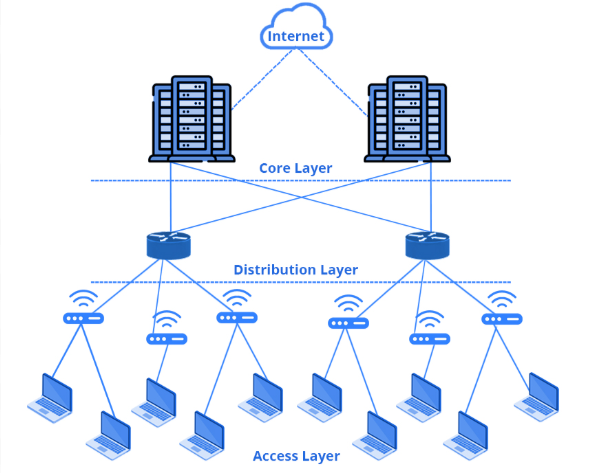
\includegraphics[width=0.5\textwidth]{figures/3tier-architecture.png}
   \caption{3-Tier Architecture}
   \label{fig:archi}
\end{figure}
\subsection{Spine-Leaf Architecture}
\hyperref[def:spineleaf]{\underline{The Spine-Leaf}} architecture is a modern two-tier model designed to overcome the limitations of the three-tier approach. It consists of spine switches that form the backbone and leaf switches that connect to end devices, with every leaf switch connected to every spine switch in a full mesh. This design guarantees that any two devices in the network are always separated by exactly two hops, delivering consistent low latency, high bandwidth, and horizontal scalability. It is widely adopted in hyperscale and cloud data centers~\cite{spine}.
\begin{figure}[htbp]
    \centering
   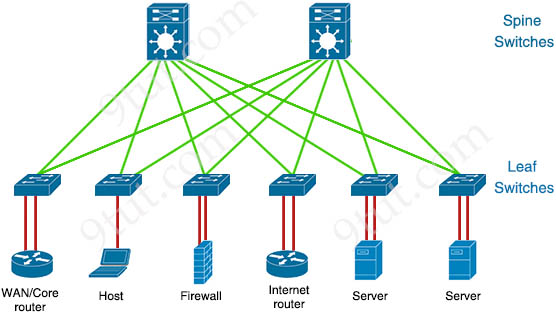
\includegraphics[width=0.5\textwidth]{figures/spine_leaf_architecture.jpg}
   \caption{Spine-Leaf Architecture}
   \label{fig:spineleaf}
\end{figure}
\section{Network Components}
\subsection{Spine Switches}
\hyperref[def:spine]{\underline{Spine switches}} form the core forwarding layer in a spine-leaf architecture. Therefore, EoR-1 and EoR-2 serve as spine switches. They connect only to leaf switches and do not connect directly to servers. Their primary role is to provide high-speed, redundant connectivity between the leaf switches, ensuring reliable and scalable traffic forwarding across the fabric.
\begin{figure}[htbp]
    \centering
   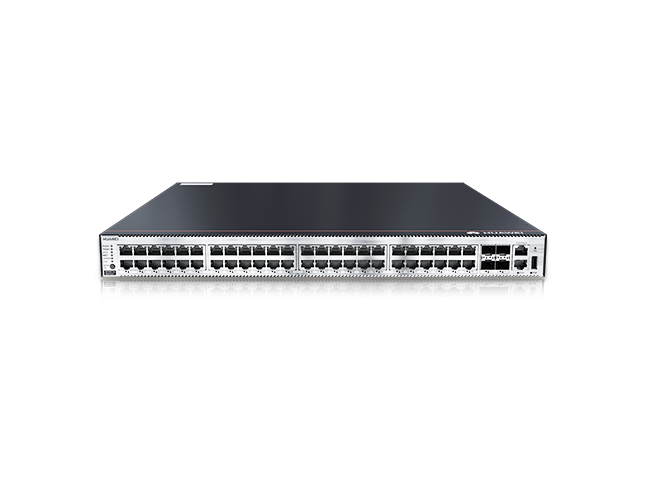
\includegraphics[width=0.3\textwidth]{figures/CloudEngine-S5731-H-v2.png}
   \caption{Huawei CloudEngine S5731 Switch Model}
   \label{fig:switch}
\end{figure}
\subsection{Leaf Switches (ToR):}
\hyperref[def:leaf]{\underline{Leaf switches}} provide server connectivity in the access layer. Positioned as Top-of-Rack switches, they connect to servers via access ports and uplink to spine switches via trunk ports. Each cabinet typically contains two leaf switches operating in active-standby mode using MLAG, with one ToR active and one standby, providing sub-second failover~\cite{switches}.
\subsection{Firewalls:}
Firewalls enforce security policies between network zones. In our design, two firewalls (FW-1 and FW-2) operate in an \hyperref[def:activestandby]{active-standby} \hyperref[def:cluster]{\underline{cluster}} at the network edge. They provide zone separation between \hyperref[def:untrust]{\underline{Untrust}} (external networks), \hyperref[def:dmz]{\underline{DMZ}}, and \hyperref[def:trust]{\underline{Trust zones}}, as well as stateful packet inspection tracking connection states. Firewalls are critical for enforcing the principle of least privilege: the DMZ can receive external traffic, but the Trust zone can only be accessed through controlled firewall rules~\cite{firewall}.
\begin{figure}[H]
    \centering
   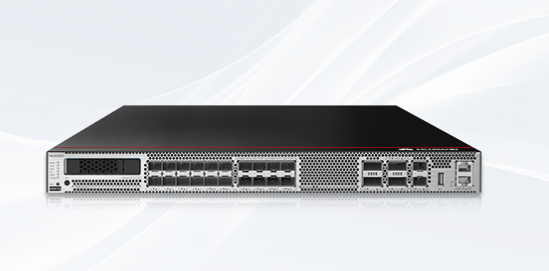
\includegraphics[width=0.3\textwidth]{figures/firewall.png}
   \caption{Huawei HiSecEngine USG6700E Firewall Model}
   \label{fig:firewall}
\end{figure}
\subsection{Servers:}
Servers host the applications and data that a data center exists to serve. The separation of management and service networks follows security best practices: administrators access management IPs for configuration, while service IPs handle application traffic. This isolation prevents management access from being exposed to the application layer~\cite{server}.
\begin{figure}[H]
    \centering
   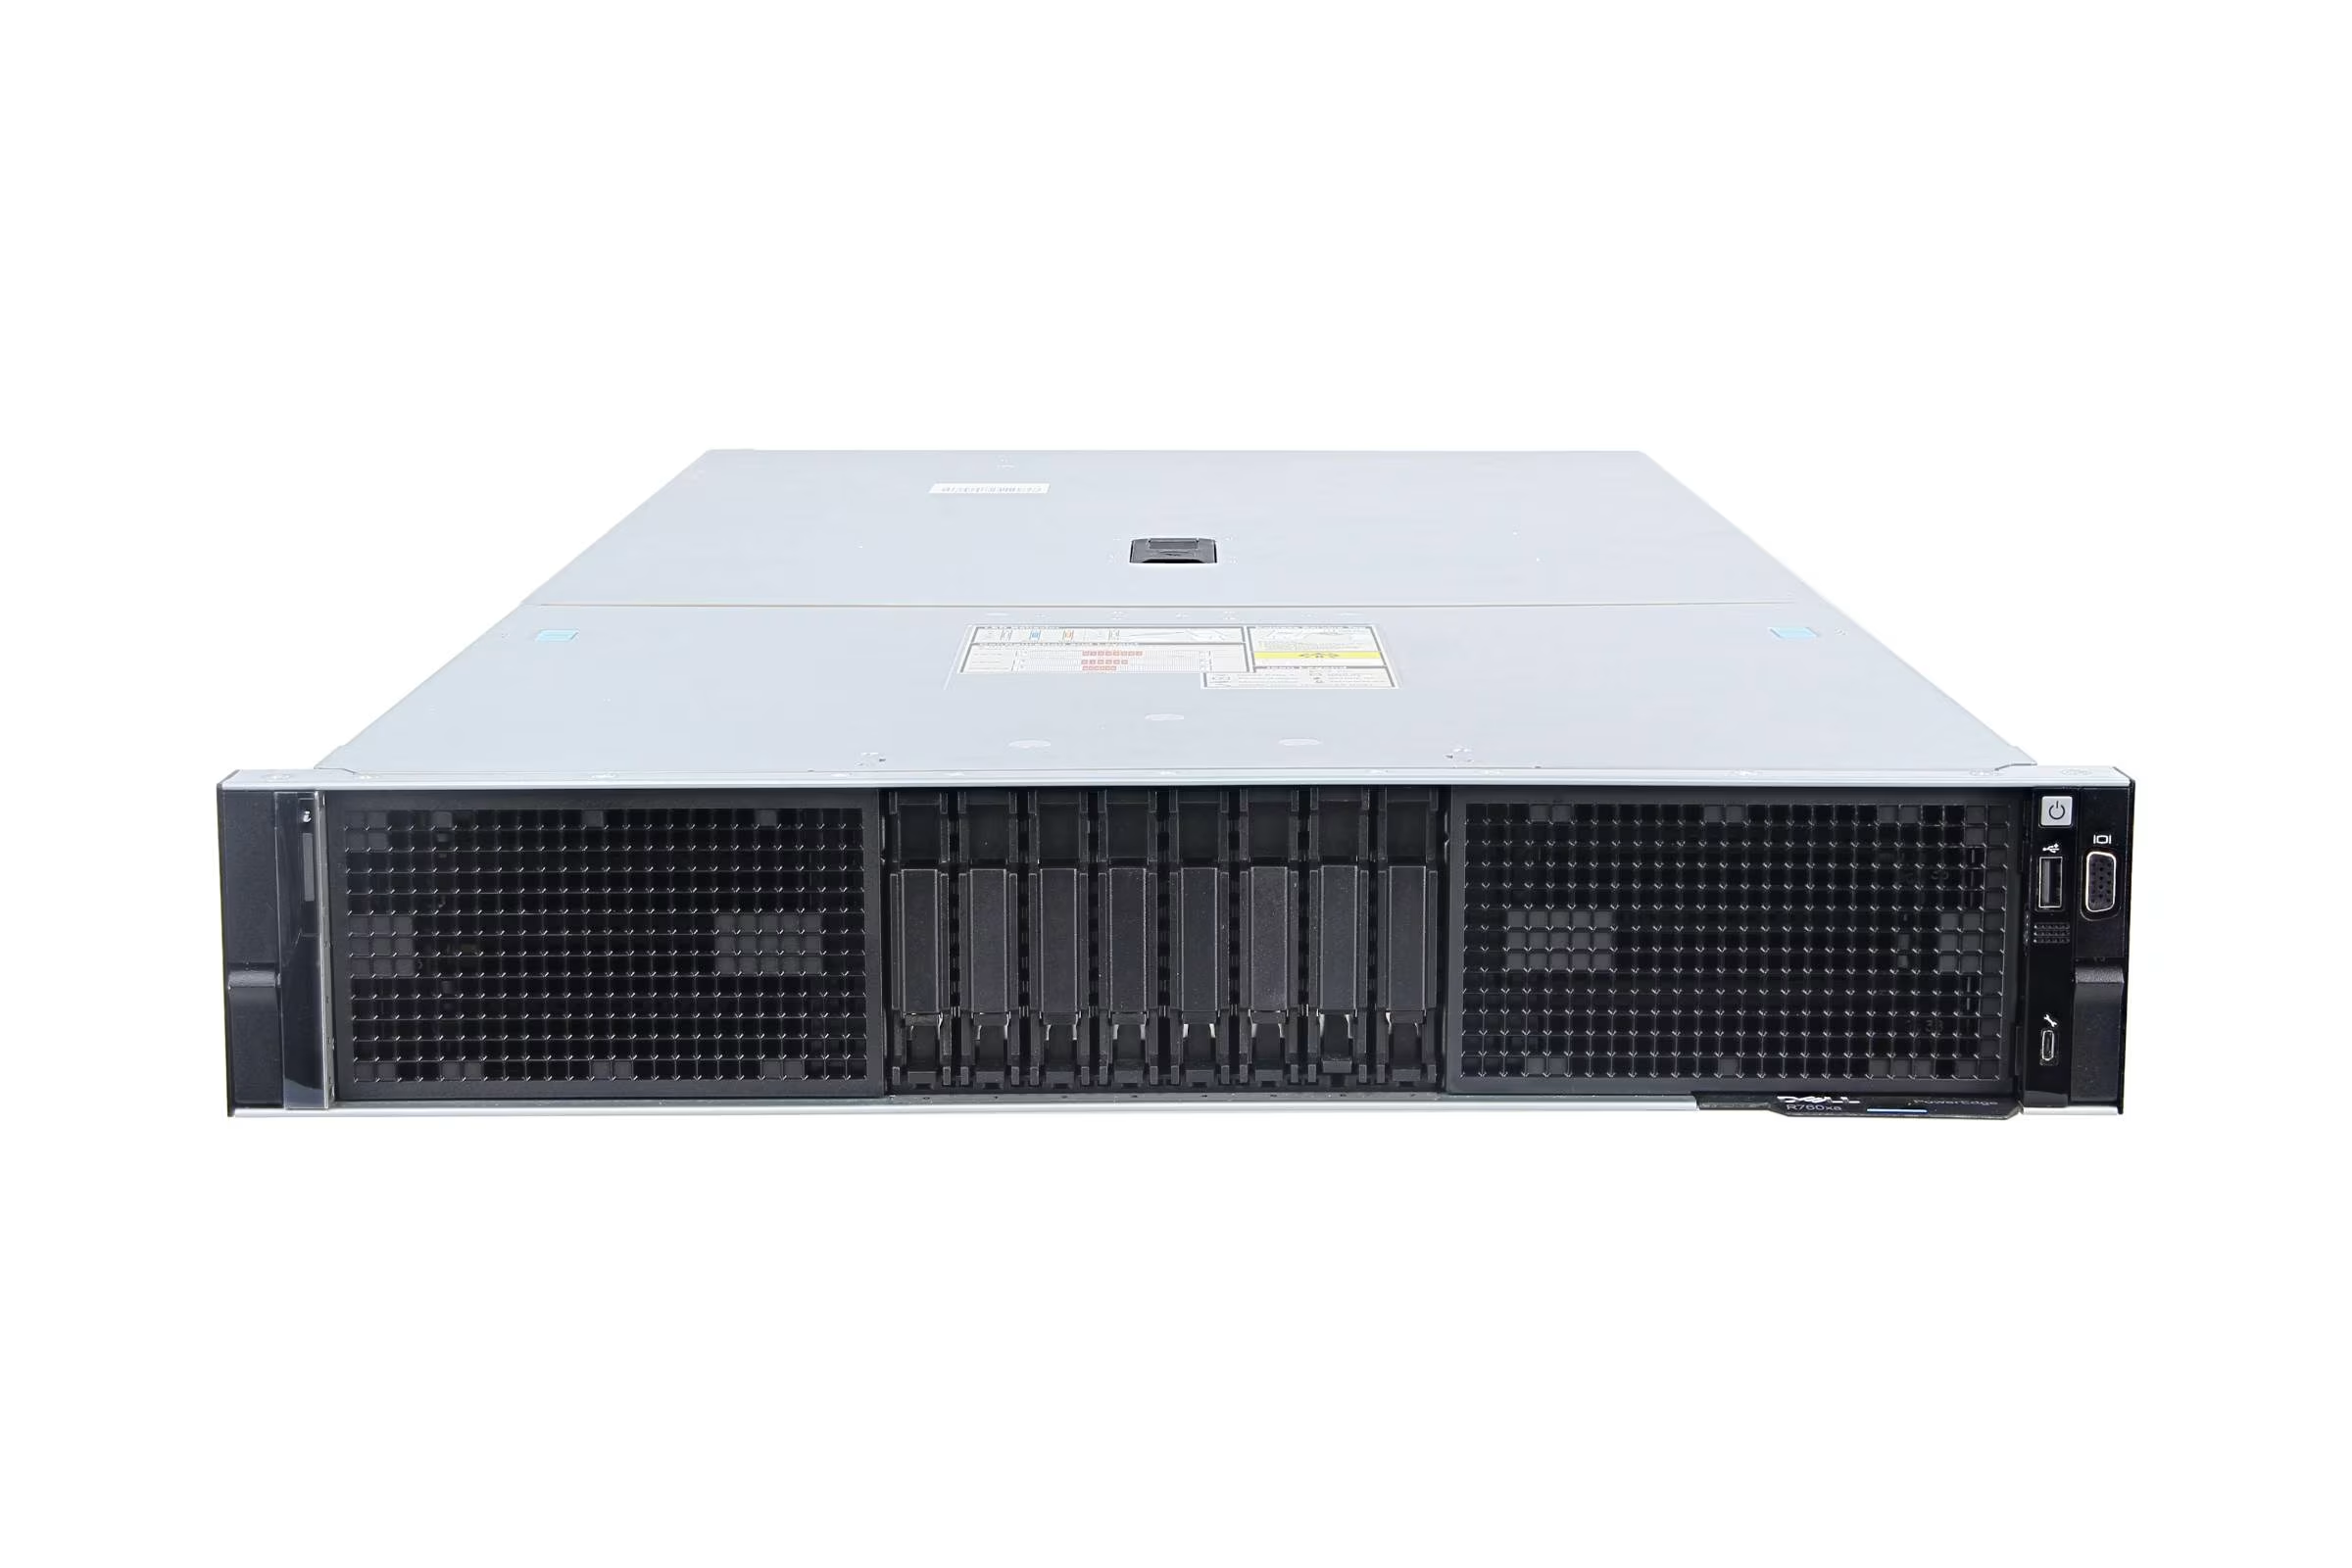
\includegraphics[width=0.3\textwidth]{figures/dell_poweredge_r760xa.png}
   \caption{Dell PowerEdge R760xa Server Model}
   \label{fig:server}
\end{figure}
\section{Core Networking Concepts}

\subsection{VLAN Segmentation and Network Zones}
A \hyperref[def:vlan]{\underline{VLAN}} logically segments a physical network into isolated broadcast domains. This improves security and reduces unnecessary traffic. In data centers, VLANs separate different traffic types such as management, storage, and application traffic. Network zones (DMZ, Trust, Untrust) extend VLAN isolation with firewall-enforced security policies. The DMZ hosts public-facing services, the Trust zone contains internal applications, and the Untrust zone represents external networks~\cite{vlan}.
\subsection{Redundancy and High Availability}
Redundancy is a fundamental principle in data center design. It ensures that the failure of a single component does not result in a service outage. In our project, redundancy is implemented at every layer of the architecture~\cite{high}:\\
  -\ \textbf{Security layer:} Two firewalls deployed in parallel, both connected to external networks and to the core switches.\\
  -\ \textbf{Spine layer:} Two EoR switches, each connected to all eight ToR switches, providing multiple forwarding paths.\\
  -\ \textbf{Leaf layer:} Each cabinet contains two ToR switches, ensuring servers remain connected even if one switch fails.\\
This multi-level redundancy guarantees high availability across the entire infrastructure using multiple protocols.
\subsection{Virtualization Principles}
Virtualization is the process of creating virtual instances of physical resources such as servers and networks. \hyperref[def:vmwareworkstation]{\underline{VMware}} is used to virtualize the IT infrastructure within each cabinet, creating virtual servers that communicate with the simulated network in \hyperref[def:pnetlab]{PNETLab}~\cite{virtu}.

\section{Conclusion}
This chapter has presented the essential concepts of modern data centers, comparing traditional Three-Tier architecture with Spine-Leaf. The analysis shows that Spine-Leaf offers consistent latency, better east-west traffic handling, and horizontal scalability, making it the preferred choice for cloud-scale infrastructures. These findings provide the theoretical basis for the design presented in the next chapter.
\chapter{Conception and Design}

\section{Introduction}
This chapter translates the theoretical spine-leaf architecture from Chapter 1 into a concrete design. We detail the topology, VLANs, IP addressing, VRRP, MLAG, security zones, and UML models. The resulting blueprint guides implementation in Chapter 3.
\section{Architecture Overview}

\subsection{Spine-Leaf Topology\hyperref[def:hld]{\underline{ (HLD)}}}
The architecture adopts a Spine-Leaf model across four virtual cabinets: A, B, C, and D. Each cabinet is equipped with two ToR switches acting as leaf nodes, giving a total of eight ToR switches at the access layer. The cabinets are interconnected through two EoR core switches acting as spine nodes, each connected to all eight ToR switches, ensuring that any server can reach any other server with minimal hops and maximum redundancy.
\subsection{Justification of Choice}
The Spine-Leaf model was chosen for this project because it reflects the architecture for modern enterprise data centers. It addresses the performance and scalability requirements of a multi-cabinet infrastructure while maintaining the security and zone separation necessary for hosting services across different trust levels, from internal database and application services to externally accessible web services in the DMZ. These choices transform a basic topology into a production-ready, carrier-grade data center blueprint.
% Landscape HLD page (rotated figure on its own page — do NOT use [H] with sidewaysfigure)
\clearpage
\thispagestyle{plain}
\begin{sidewaysfigure}[p]
    \centering
    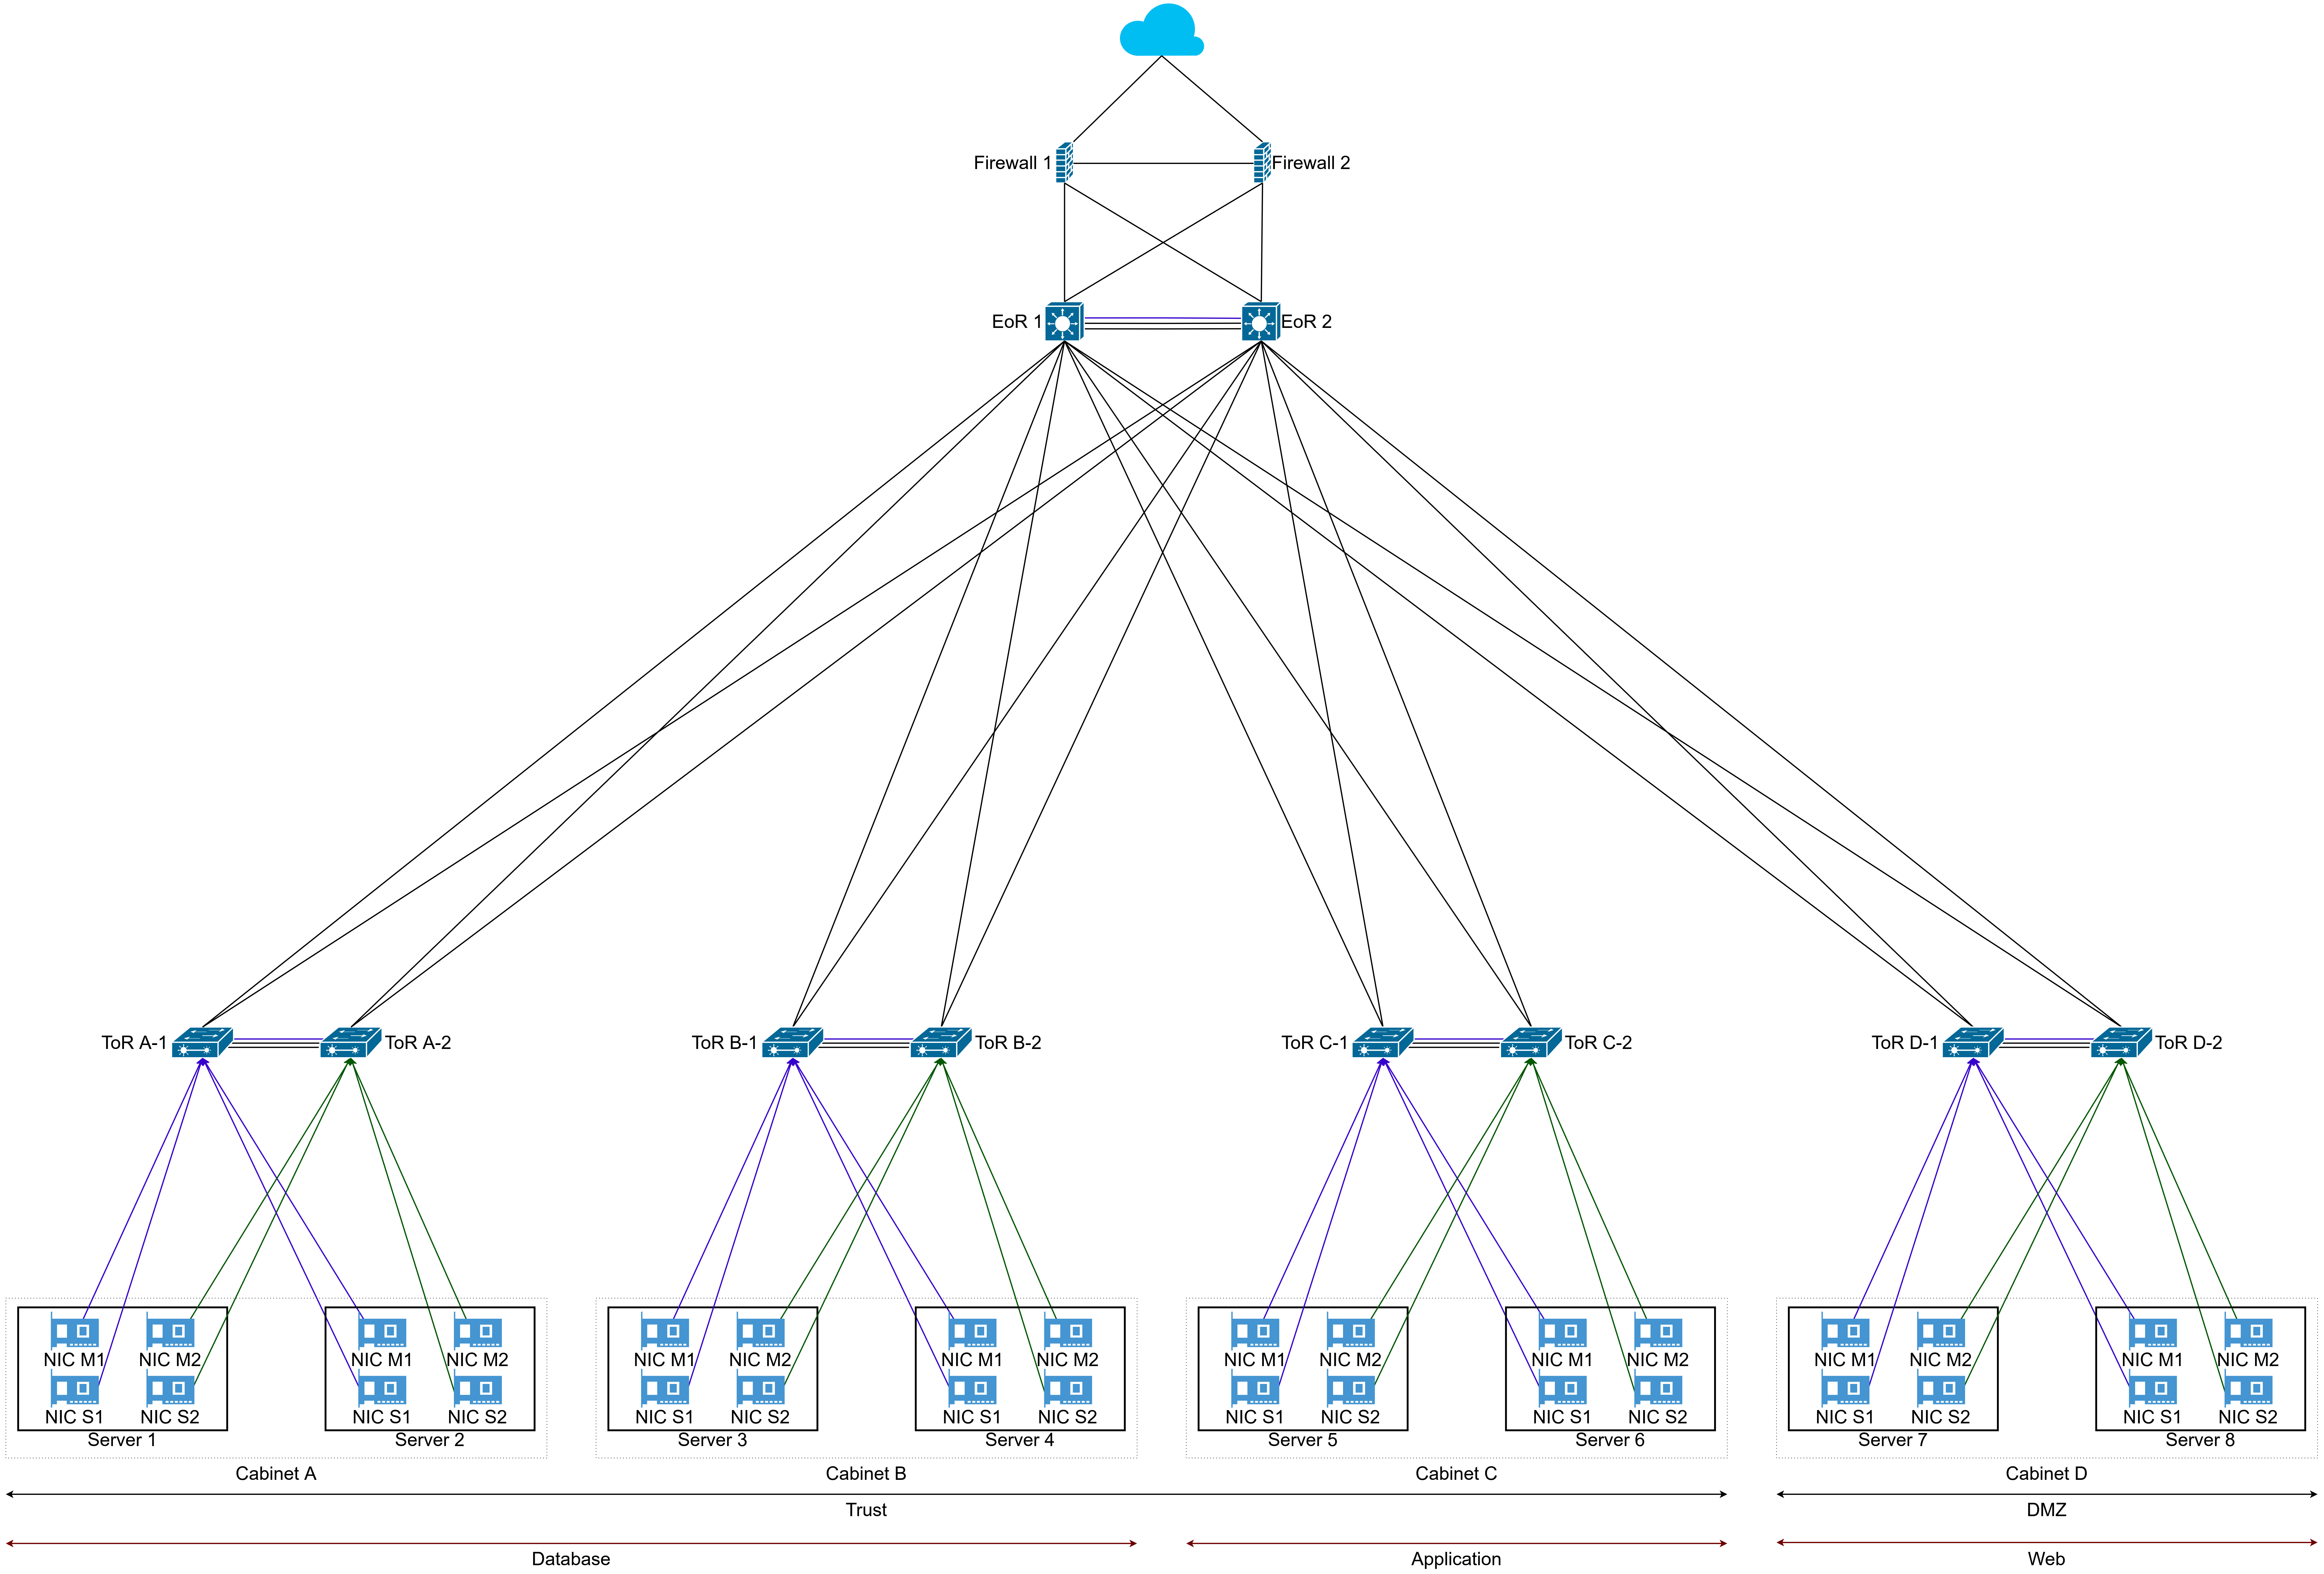
\includegraphics[width=0.92\textheight,keepaspectratio]{figures/HLDV4.drawio.png}
    \caption{Spine-Leaf topology of the proposed data center.}
    \label{fig:topology}
\end{sidewaysfigure}
\FloatBarrier
\clearpage

\subsection{Leaf Layer}
\begin{figure}[H]
    \centering
    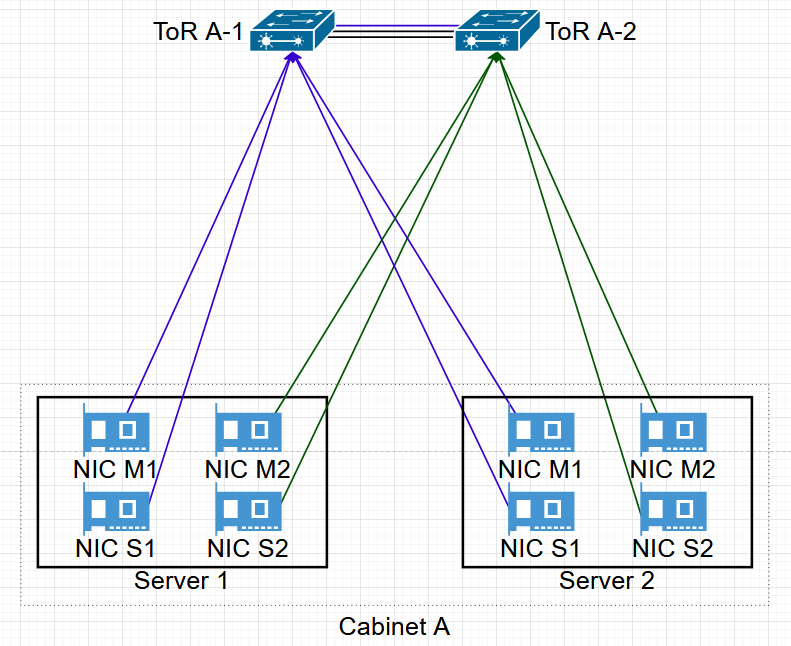
\includegraphics[width=0.45\textwidth,interpolate=false]{figures/leaf_layer.png}
    \caption{Leaf Layer}
    \label{fig:leaf-layer}
\end{figure}
\textbf{1. Cabinets and Servers:} The physical infrastructure consists of four server cabinets (A, B, C, and D). Each cabinet houses two servers, resulting in a total of eight physical servers. Cabinet A contains Servers 1 and 2; Cabinet B contains Servers 3 and 4; Cabinet C contains Servers 5 and 6; Cabinet D contains Servers 7 and 8.\\
Each server contains two active network cards (\hyperref[def:management]{\underline{M1}} and \hyperref[def:service]{\underline{S1}}) and two backup network cards (M2 and S2):\\
- M: Management network card, used by the system administrator to access the server for configuration.\\
- S: Service network card, used for application and production traffic between servers and services.\\
\textbf{2. ToR Switches:} Each cabinet is served by two ToR switches, one active and one standby, providing local connectivity for the servers within that cabinet. In each cabinet:\\
- ToR X-1 (active) connects to the two active network cards (M1 and S1) in the two servers in that cabinet.\\
- ToR X-2 (standby) connects to the two backup network cards (M2 and S2) in the two servers in that cabinet.\\
ToRs A-Y connect to the two servers in Cabinet A, ToRs B-Y connect to the two servers in Cabinet B, ToRs C-Y connect to the two servers in Cabinet C, ToRs D-Y connect to the two servers in Cabinet D.
\subsection{Spine Layer}
\begin{figure}[H]
    \centering
    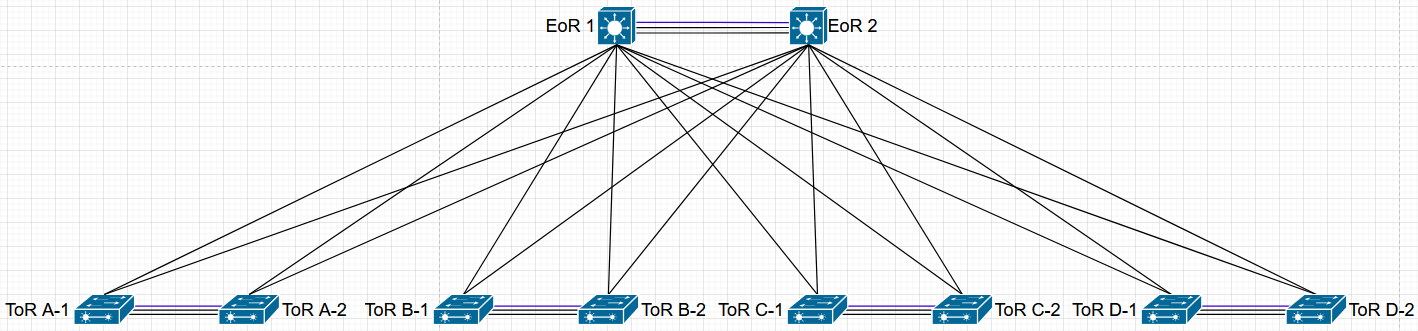
\includegraphics[width=0.75\textwidth,interpolate=false]{figures/spine_layer.png}
    \caption{Spine Layer}
    \label{fig:spine-layer}
\end{figure}
\textbf{EoR Switches}: All ToR switches uplink to the core layer, which consists of two End of Row (EoR) switches. These serve as the aggregation point for the entire server farm.\\
- EoR 1 and EoR 2 are configured in a high-availability (active/standby) pair.\\
- Each ToR maintains a connection to both EoR 1 and EoR 2. This ensures that if the active path fails, traffic can instantly switch to the standby core switch.\\
- A direct link exists between EoR 1 and EoR 2 to facilitate synchronization and failover detection (heartbeat).
\subsection{Network Edge}
\begin{figure}[H]
    \centering
    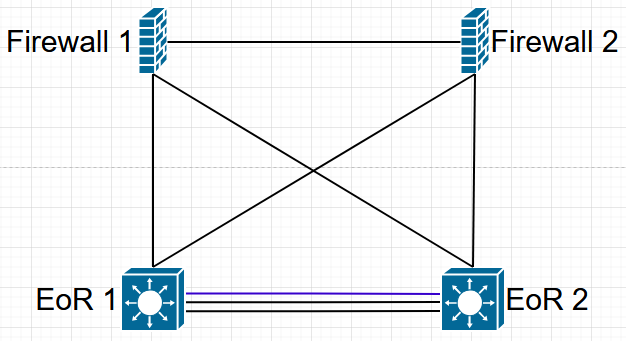
\includegraphics[width=0.45\textwidth,interpolate=false]{figures/network_edge.png}
    \caption{Network Edge}
    \label{fig:network-edge}
\end{figure}
\textbf{Firewalls:} The core switches connect directly to the network security layer, which is comprised of a pair of firewalls.\\
- Firewall 1 (Active) and Firewall 2 (Standby) provide north-south security for the server traffic.\\
- Both EoR 1 and EoR 2 are connected to both Firewall 1 and Firewall 2, eliminating a single point of failure in the uplink path.\\
- A direct link connects Firewall 1 and Firewall 2 to maintain session state synchronization and monitor health for seamless failover.\\
\subsection{Cloud Connection}
\begin{figure}[H]
    \centering
    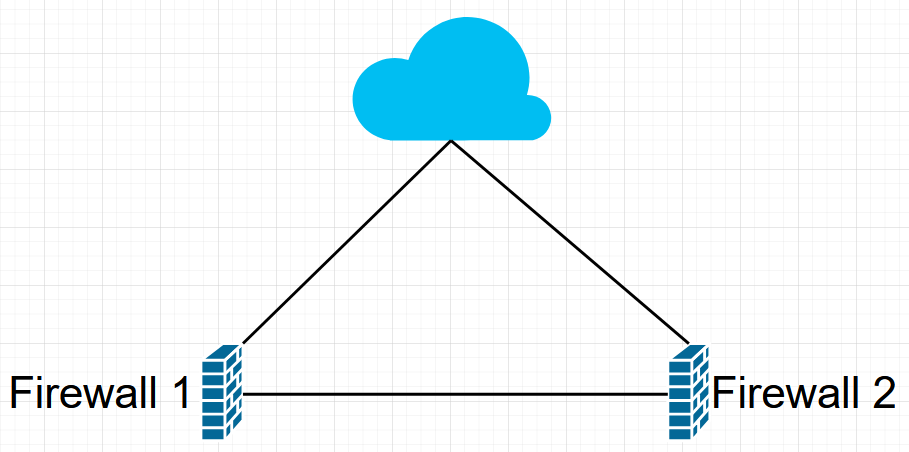
\includegraphics[width=0.45\textwidth,interpolate=false]{figures/cloud_connection.png}
    \caption{External cloud and network access}
    \label{fig:cloud-edge}
\end{figure}
The two perimeter firewalls connect the internal network to the external cloud network. All inbound and outbound traffic between the internal environment and the external network traverses these firewalls, where untrusted traffic is inspected and filtered according to security policies.\\
\subsection{Cabinet Structure}
The physical architecture is organized into four cabinets, each representing a specific function and security zone:

\begin{table}[htbp]
    \centering
    \caption{Cabinet organization by zone and function}
    \label{tab:cabinets}
    \begin{tabular}{|c|c|c|c|c|c|}
        \hline
        \textbf{Cabinet} & \textbf{Zone} & \textbf{Function} & \textbf{Servers} & \textbf{ToR Pair} & \textbf{VLANs} \\
        \hline
        A & Trust & Database & 2 servers & A-1, A-2 & 110, 120 \\
        B & Trust & Database & 2 servers & B-1, B-2 & 110, 120 \\
        C & Trust & Application & 2 servers & C-1, C-2 & 110, 130 \\
        D & DMZ & Web & 2 servers & D-1, D-2 & 210, 220 \\
        \hline
    \end{tabular}
\end{table}
Each cabinet contains two servers with four \hyperref[def:nic]{\underline{NICs}} per server and two ToR switches. The ToR switches are configured as an MLAG pair, operating in active-standby mode with one switch active and one standby.
 \section{Requirements Specification}
 \subsection{Actors:}
The system supports several categories of actors, each with rights and responsibilities adapted to their role. Six primary actors interact with the data center system, as summarized in Table~\ref{tab:actors}.

\begin{table}[htbp]
    \centering
    \caption{Primary actors of the data center system}
    \label{tab:actors}
    \begin{tabular}{|l|p{0.62\textwidth}|}
        \hline
        \textbf{Actor} & \textbf{Role and responsibilities} \\
        \hline
        External User & Client accessing web services hosted in the DMZ zone via HTTPS. \\
        \hline
        IT Administrator & Performs user authentication and monitors cabinet health across all four cabinets. \\
        \hline
        Network Admin & Configures switches, VLANs, VRRP redundancy, MLAG active-standby pairs, and trunk/access ports. \\
        \hline
        System Admin & Manages server virtual machines and multi-NIC configuration on Linux servers. \\
        \hline
        Security Admin & Manages firewall rules and enforces DMZ/Trust zone separation with default-deny policies. \\
        \hline
        Super Admin & Has full system access and inherits all capabilities from Network, System, Security, and IT Administrators. \\
        \hline
    \end{tabular}
\end{table}
\subsection{Functional Requirements}
The data center must fulfill the following functional requirements:\\
- The system must isolate web servers from application and database servers using firewall-enforced DMZ and Trust zones.\\
- The system must provide redundant gateway IPs so that server connectivity continues in case of failure.\\
- The system must support automatic failover between redundant ToRs, EoRs and firewalls with zero packet loss.\\
- The system must allow IT administrators to remotely configure all network devices via SSH on a dedicated management VLAN.\\
- The system should be ready for clients to deploy their own applications (web, application, and database) on the infrastructure.
\subsection{Non-Functional Requirements}
Non-functional requirements define the quality expectations and overall constraints of the data center. The main non-functional requirements identified are:\\
- \textbf{Redundancy:} No single point of failure at any layer. Spine, leaf, servers, and firewalls must all have redundancy.\\
- \textbf{Security:} DMZ and Trust zones must be strictly separated by firewall policies with default-deny rules.\\
- \textbf{Scalability:} The architecture must support adding additional cabinets without redesigning the network.\\
- \textbf{Manageability:} All devices must be accessible via SSH on a dedicated management network (VLAN~110 and VLAN~210).

\subsection{Choice of Modeling Language}
We chose \hyperref[def:uml]{\underline{UML}} (Unified Modeling Language) to model our system because of its robustness and wide adoption. This language supports the representation of many kinds of systems, especially IT systems, through its object-oriented approach. UML offers strong expressiveness for capturing requirements from several perspectives; we emphasize the functional view through use case diagrams.
\subsection{Use Case Description}
Figure~\ref{fig:usecase} presents the \hyperref[def:usecase]{\underline{use case}} diagram with six actors: External User, Network Admin, System Admin, Security Admin, IT Admin, and Super Admin. Use cases cover DMZ access, network configuration (\hyperref[def:vlan]{\underline{VLAN}}, \hyperref[def:vrrp]{\underline{VRRP}}, \hyperref[def:mlag]{\underline{MLAG}}), server management, security, and system management. \texttt{<<include>>} arrows require authentication for all configuration actions, while \texttt{<<extend>>} arrows show optional behaviors. Generalization arrows show Super Admin inherits from all other admins.\\
\subsection{Use Case Diagram}
% IMAGE: media/image3.png - Use case diagram
 \begin{figure}[H]
    \centering
   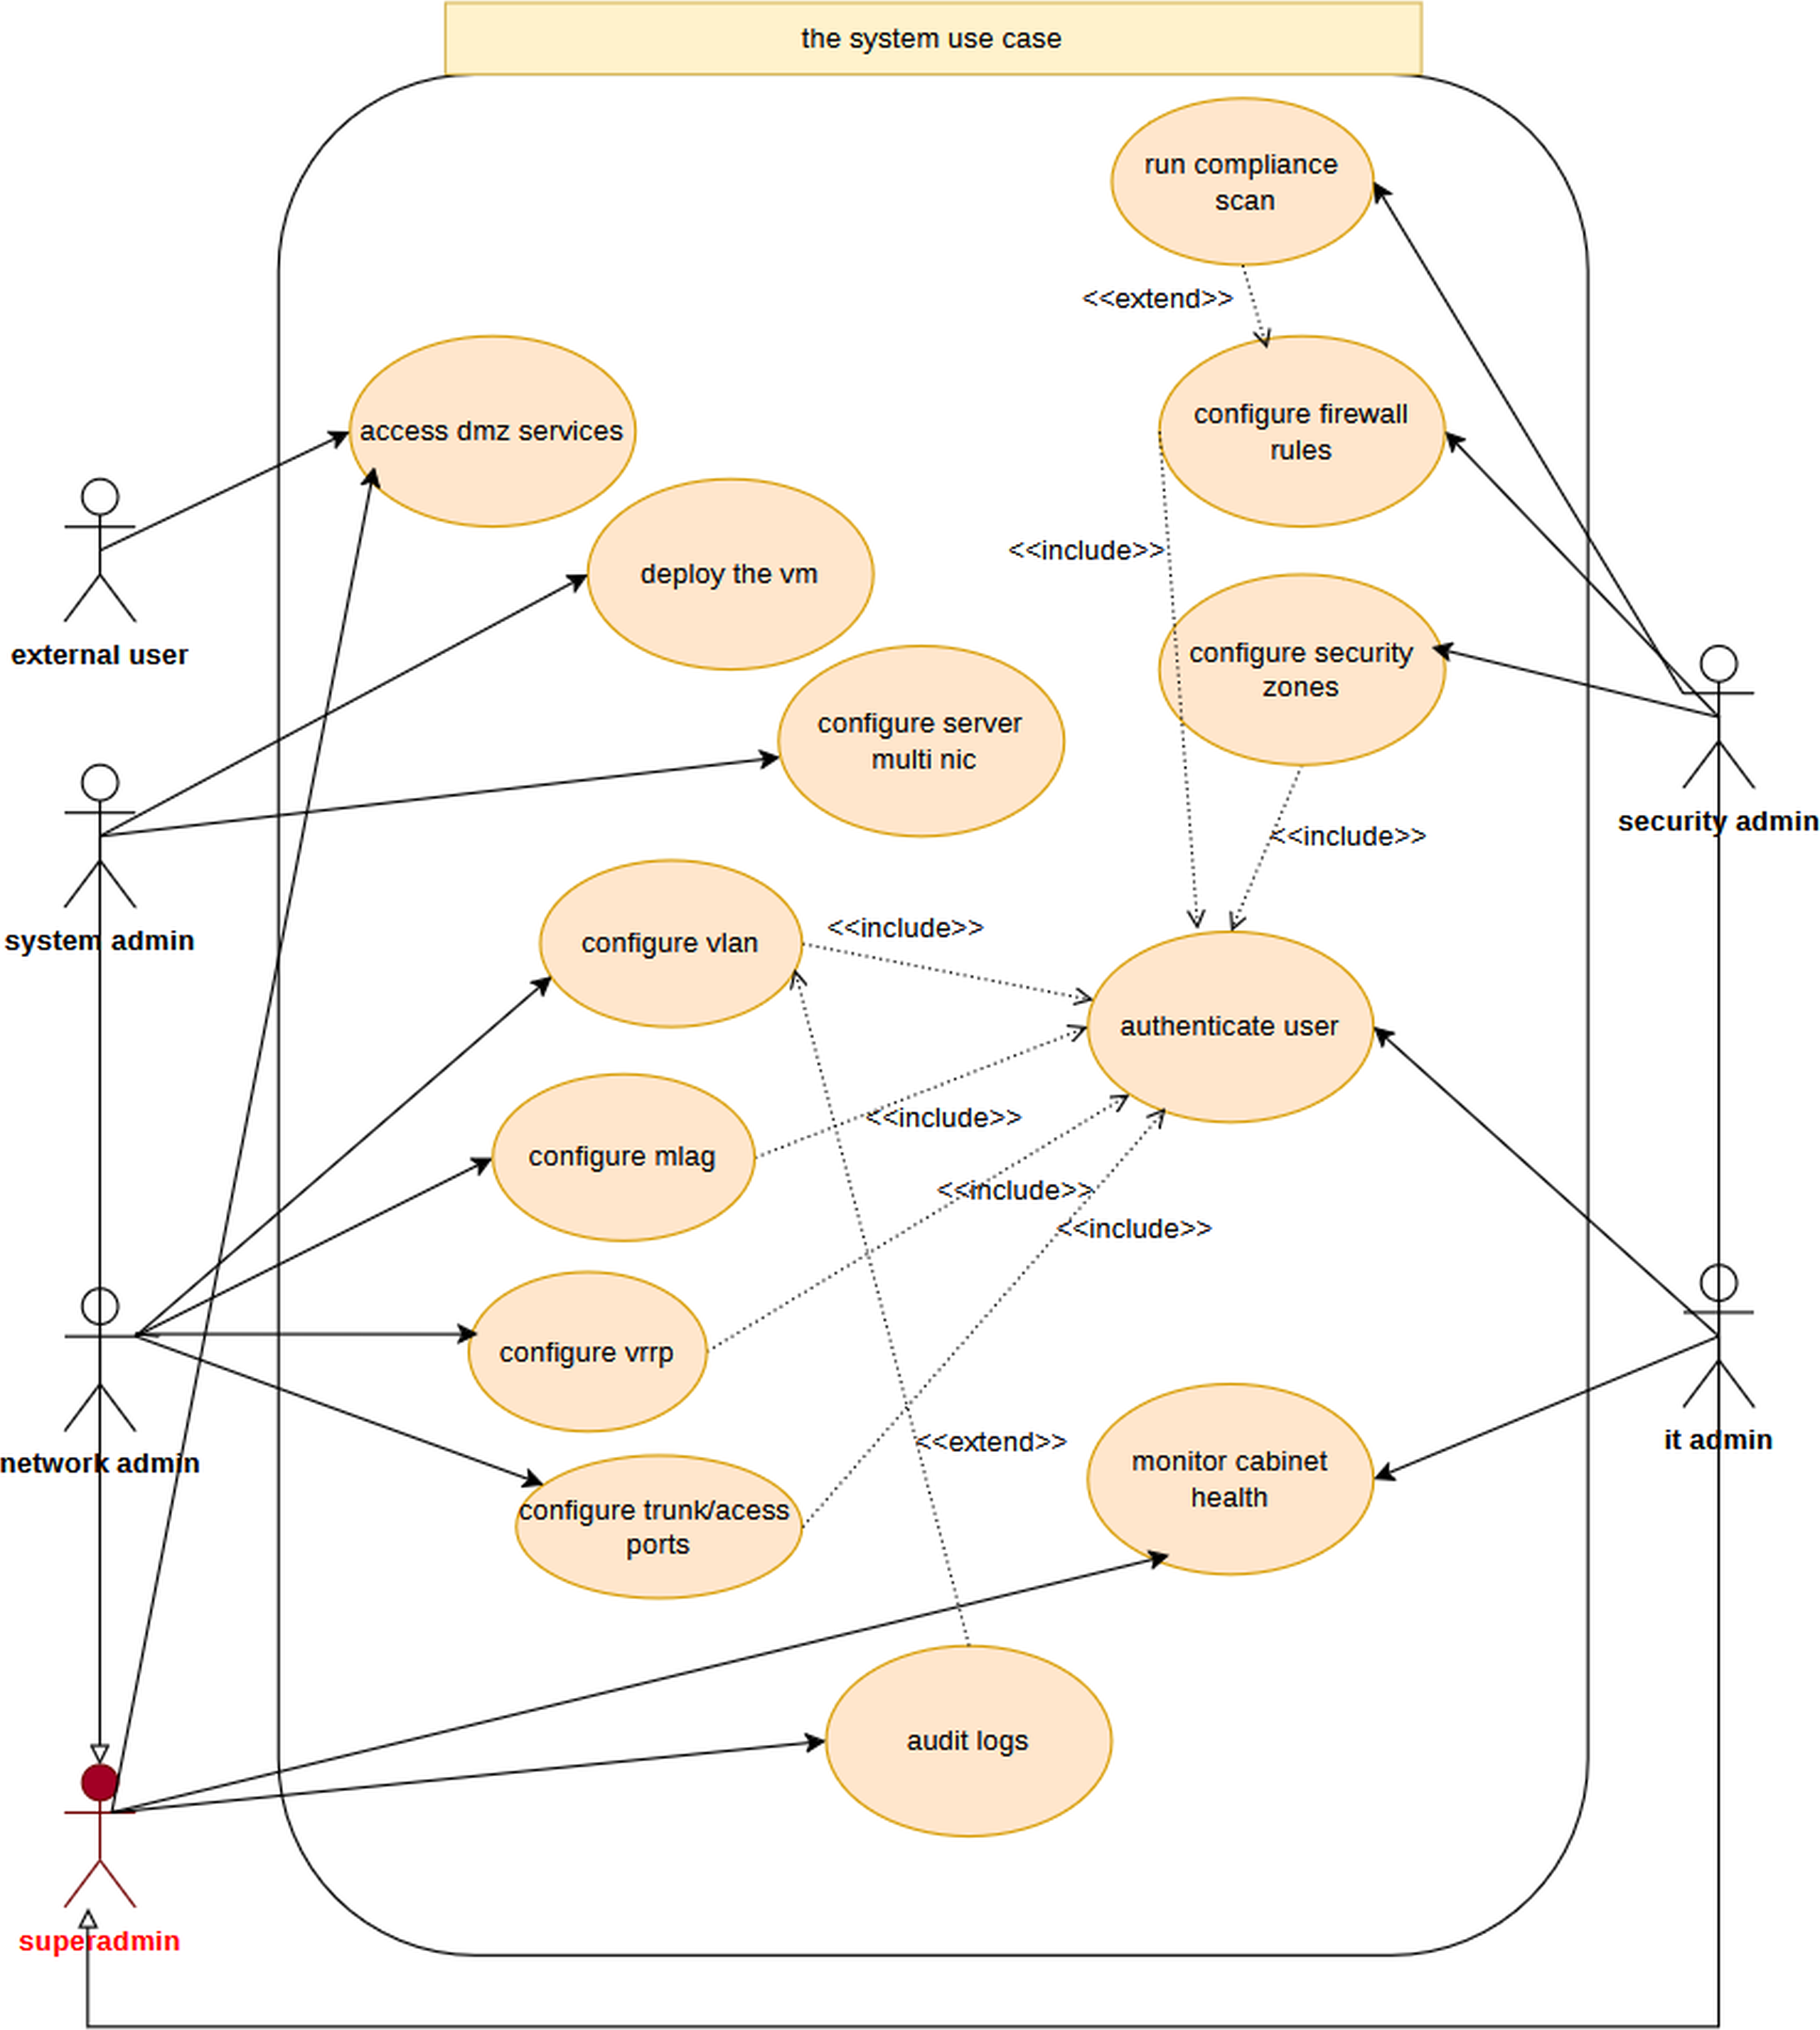
\includegraphics[width=0.72\textwidth,interpolate=false]{figures/newuse.png}
   \caption{Use case diagram of the data center system.}
  \label{fig:usecase}
 \end{figure}
The diagram presents all actors interacting with the data center network architecture. Actors are categorized by their access zone and authentication method.
\section{Sequence Diagrams}
\subsection{Network Administrator Configuring EoR Spine Switches}
The sequence diagram in Figure~\ref{fig:sequence-eor} illustrates the steps a network administrator follows to configure the EoR spine switches (EoR-1 and EoR-2): initial SSH setup, MLAG peer configuration, and downlink binding to ToR switches per cabinet.\\
 \begin{figure}[H]
     \centering
    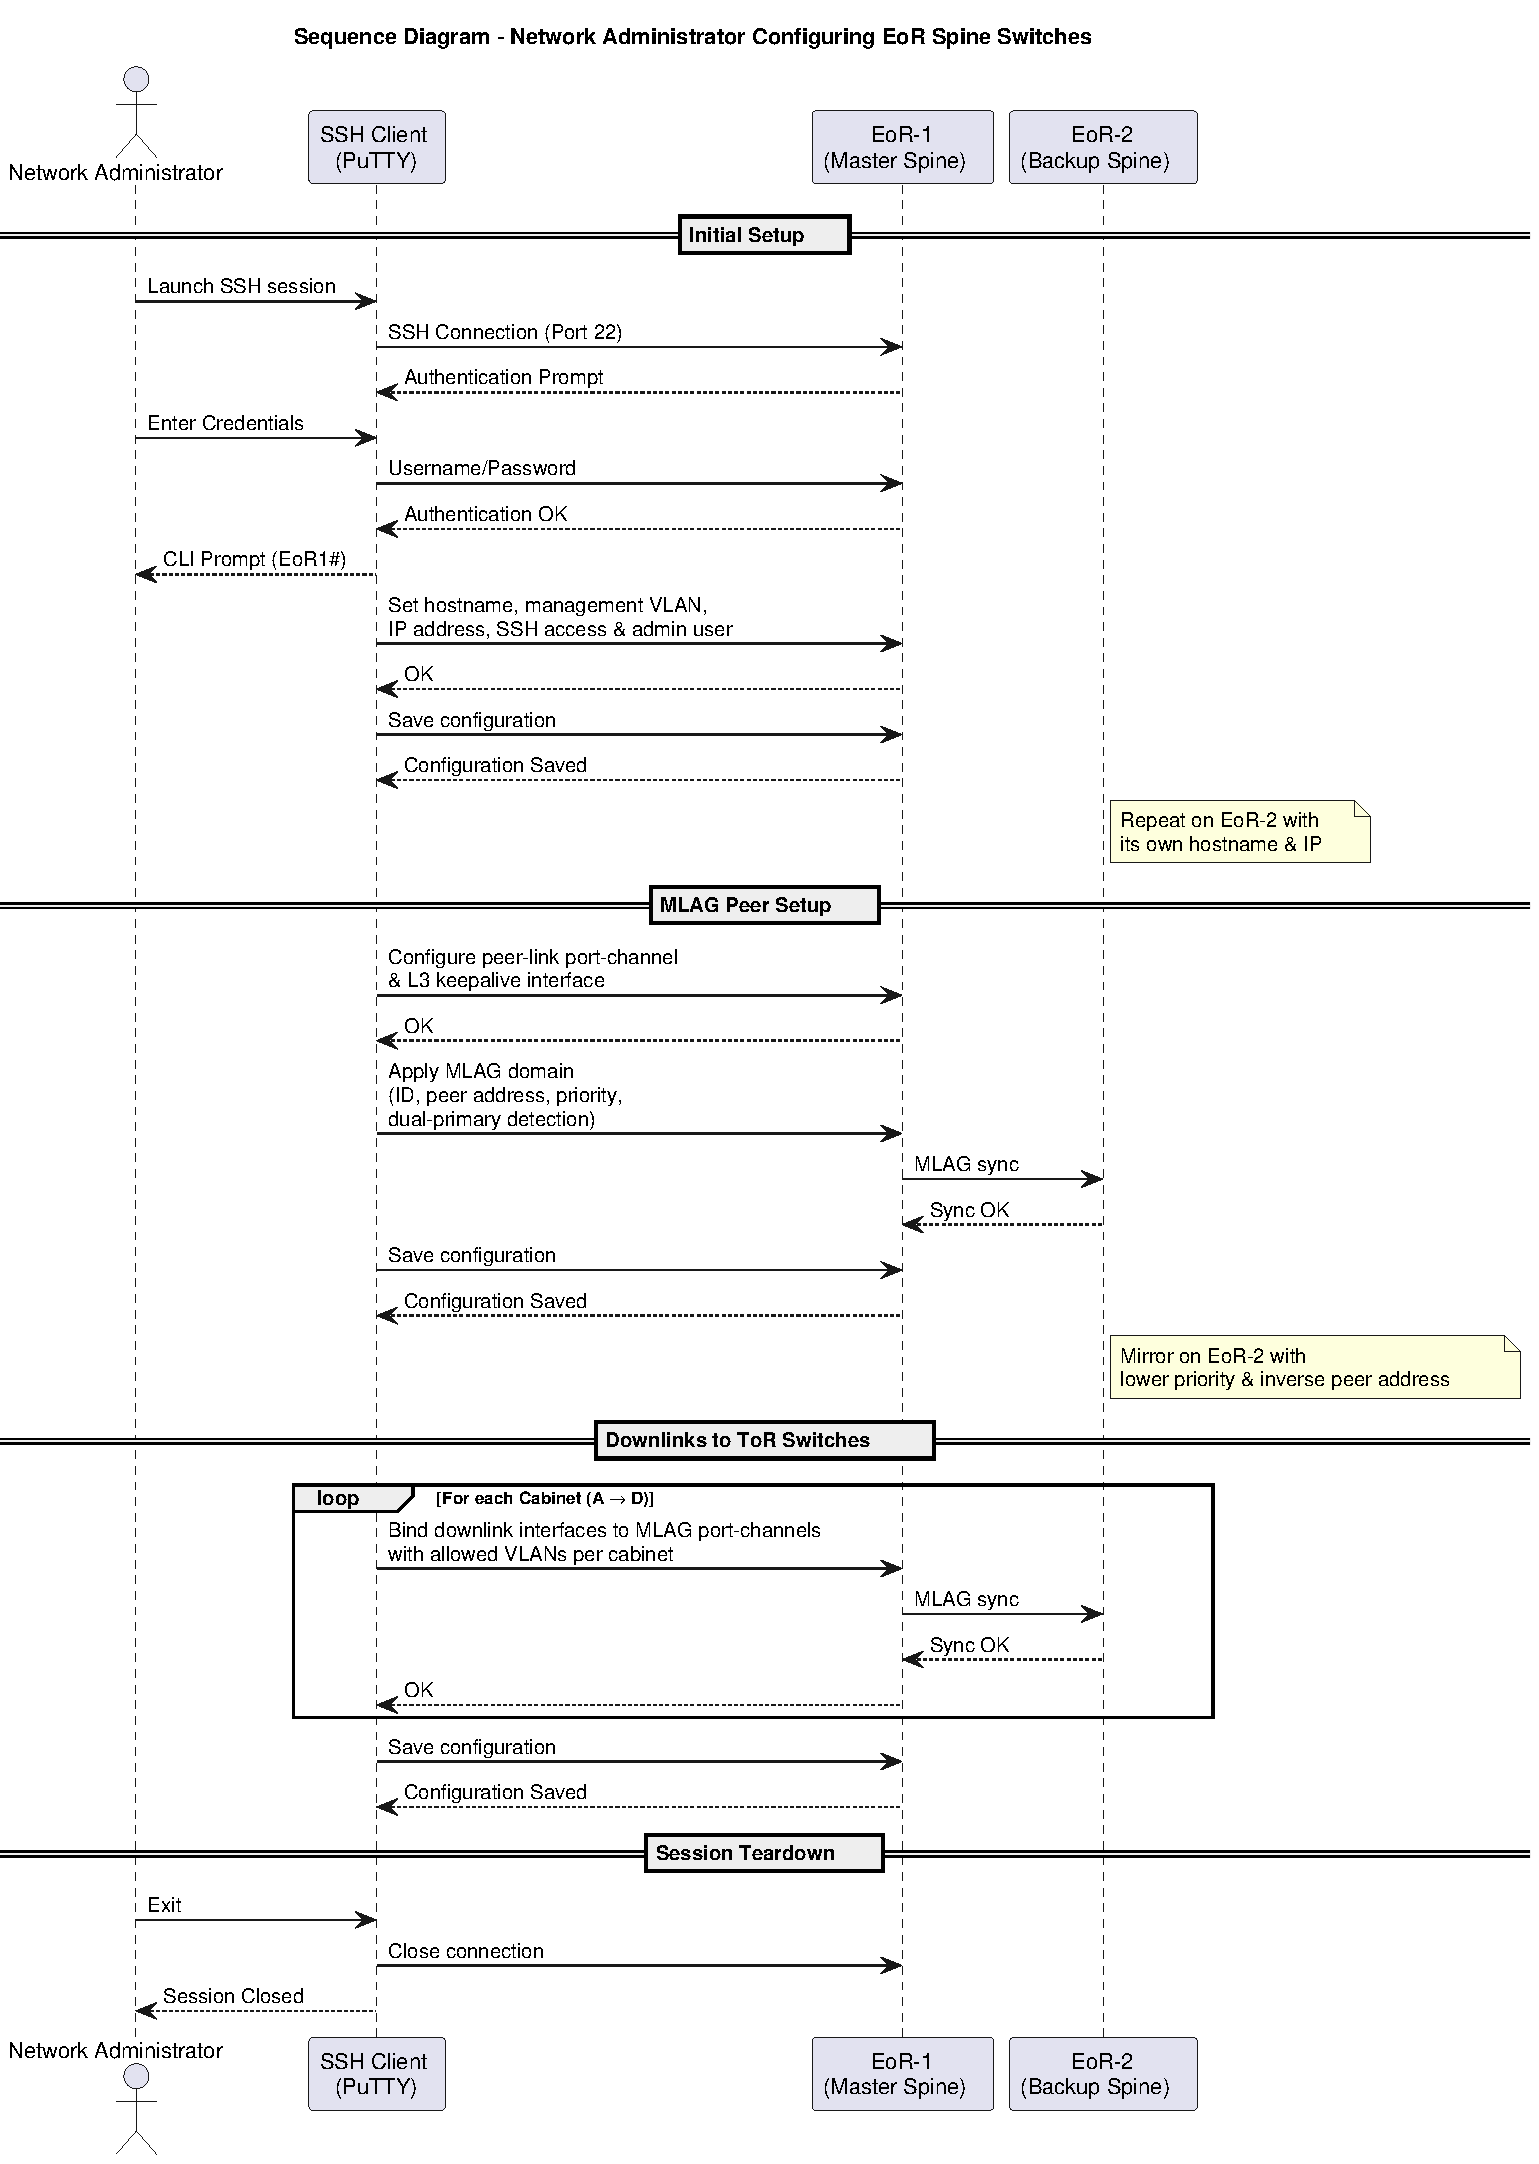
\includegraphics[width=0.88\textwidth,height=0.58\textheight,keepaspectratio]{figures/eor_config_sequence.pdf}
    \caption{Sequence diagram: Network administrator configuring EoR spine switches.}
    \label{fig:sequence-eor}
 \end{figure}

\subsection{System Administrator Configuring a Server}
The sequence diagram in Figure~\ref{fig:sequence-server} illustrates the steps a system administrator follows to configure a Linux server: SSH connection, enabling bonding and 802.1Q kernel modules, configuring physical interfaces, creating \texttt{bond0} (management, VLAN~110) and \texttt{bond1} (service, VLAN~120) with active-backup slaves, and verifying interface reachability before session teardown.\\
 \begin{figure}[H]
     \centering
    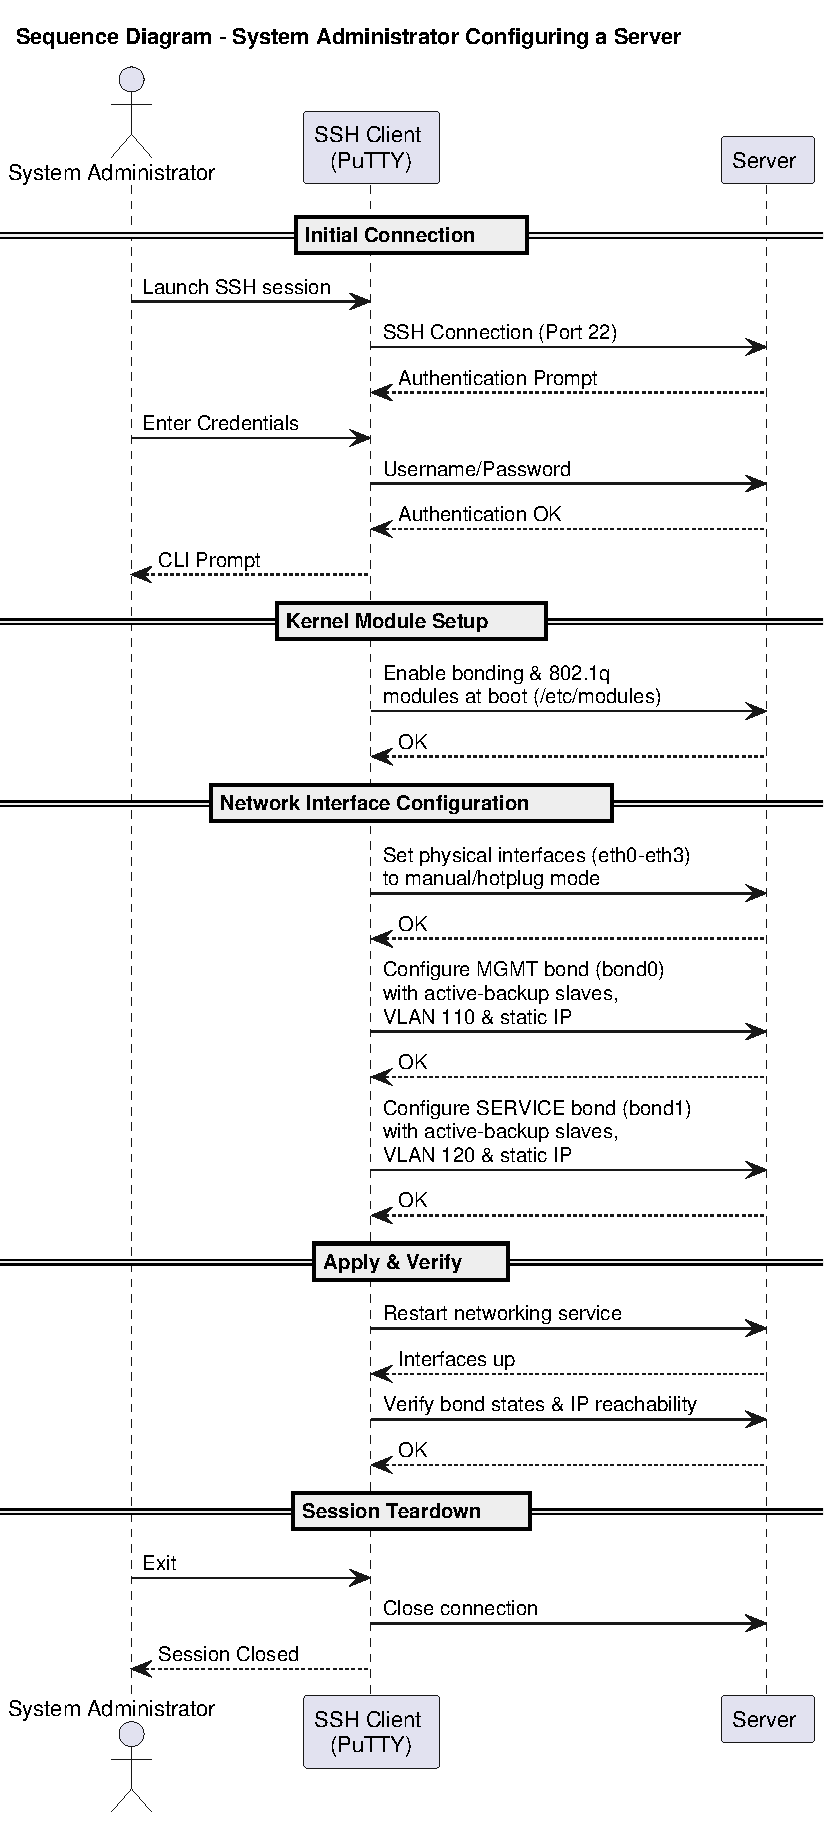
\includegraphics[width=0.88\textwidth,height=0.58\textheight,keepaspectratio]{figures/server_config_sequence.pdf}
    \caption{Sequence diagram: System administrator configuring a server.}
    \label{fig:sequence-server}
 \end{figure}
\section{Low-Level Design (LLD)}

\subsection{Device inventory}
The data center comprises 2 spine switches, 8 leaf switches, 2 firewalls, and 8 servers. Table~\ref{tab:device-inventory-sample} shows one representative device per type; the full inventory is in Appendix~\ref{app:lld}, Figure~\ref{fig:app-device-inventory}.

\begin{table}[htbp]
    \centering
    \small
    \caption{Sample device inventory (one device per type)}
    \label{tab:device-inventory-sample}
    \begin{tabular}{|l|l|l|l|}
        \hline
        \textbf{Device} & \textbf{Model/OS} & \textbf{Role} & \textbf{Location} \\
        \hline
        EoR-1 & Arista vEOS & Spine switch & Core rack \\
        ToR A-1 & Arista vEOS & Leaf switch & Cabinet A \\
        FW-1 & pfSense & Firewall & Core rack \\
        Server 1 & Linux & Database server & Cabinet A \\
        \hline
    \end{tabular}
\end{table}

\subsection{Port connections}
Physical cabling between EoR, ToR, firewall, and server ports is summarized below for one representative path (ToR A-1, EoR-1, FW-1, Server~1). The complete matrices are in Appendix~\ref{app:lld}, Figures~\ref{fig:app-port-conn-1}--\ref{fig:app-port-conn-3}.

\begin{table}[H]
    \centering
    \footnotesize
    \caption{ToR A-1 $\rightarrow$ Server 1 (access, copper trunk).}
    \label{tab:lld-port-tor-server}
    \begin{tabular}{|l|l|l|l|c|}
        \hline
        \textbf{Source port} & \textbf{Type} & \textbf{Destination} & \textbf{Dest.\ port} & \textbf{VLAN} \\
        \hline
        Ethernet0/0/1 & Access & Server 1 & NIC M1 & 110 \\
        Ethernet0/0/2 & Access & Server 1 & NIC S1 & 120 \\
        \hline
    \end{tabular}
\end{table}

\begin{table}[H]
    \centering
    \footnotesize
    \caption{ToR A-1 $\rightarrow$ EoR-1 (uplink, fiber trunk).}
    \label{tab:lld-port-tor-eor}
    \begin{tabular}{|l|l|l|l|c|}
        \hline
        \textbf{Source port} & \textbf{Type} & \textbf{Destination} & \textbf{Dest.\ port} & \textbf{VLANs} \\
        \hline
        GigabitEthernet0/0/1 & Trunk & EoR-1 & GigabitEthernet0/0/1 & 110, 120, 130 \\
        \hline
    \end{tabular}
\end{table}

\begin{table}[H]
    \centering
    \footnotesize
    \caption{EoR-1 $\rightarrow$ FW-1 (edge, fiber trunk).}
    \label{tab:lld-port-eor-fw}
    \begin{tabular}{|l|l|l|l|c|}
        \hline
        \textbf{Source port} & \textbf{Type} & \textbf{Destination} & \textbf{Dest.\ port} & \textbf{VLANs} \\
        \hline
        GigabitEthernet0/0/24 & Trunk & FW-1 & GigabitEthernet1/0/0 & 110, 120, 130, 210, 220 \\
        \hline
    \end{tabular}
\end{table}

Each ToR uplinks to both EoR switches; both EoRs connect to both firewalls; servers dual-home to their cabinet ToR pair.
\hyperref[def:trunk]{\underline{Trunk ports}} carry multiple VLANs between switches. Spine-to-leaf, spine-to-spine, and spine-to-firewall trunks carry all five VLANs (110, 120, 130, 210, 220).

\subsection{VLAN Design}
Based on the security zone requirements and traffic separation needs, we defined the following VLANs from the LLD:
 \begin{figure}[H]
    \centering
   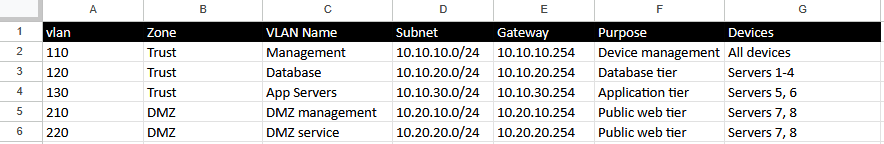
\includegraphics[width=0.72\textwidth,interpolate=false]{figures/vlan.png}
    \caption{VLAN assignment table.}
\label{fig:vlan}
 \end{figure}
All VLANs use /24 subnets (254 usable addresses), providing sufficient capacity for current needs and future expansion.

\subsection{Server IP Assignments}
Each server uses \texttt{bond0} (M1+M2) for management traffic and \texttt{bond1} (S1+S2) for service traffic. ToR and EoR switches use a management SVI on VLAN~110; firewalls use \texttt{lagg0} sub-interfaces per VLAN. Table~\ref{tab:ip-plan-sample} lists one example per device type (IP and interface); the complete plan is in Appendix~\ref{app:lld}, Figure~\ref{fig:app-ip-plan}.

\begin{table}[H]
    \centering
    \scriptsize
    \caption{Sample IP and interface assignments (one device per type).}
    \label{tab:ip-plan-sample}
    \setlength{\tabcolsep}{4pt}
    \renewcommand{\arraystretch}{1.05}
    \resizebox{\textwidth}{!}{%
    \begin{tabular}{|l|cc|cc|cc|cc|cc|}
        \hline
        \textbf{Device} &
        \multicolumn{2}{c|}{\textbf{V110 (mgmt)}} &
        \multicolumn{2}{c|}{\textbf{V120 (DB)}} &
        \multicolumn{2}{c|}{\textbf{V130 (app)}} &
        \multicolumn{2}{c|}{\textbf{V210 (DMZ mgmt)}} &
        \multicolumn{2}{c|}{\textbf{V220 (DMZ web)}} \\
        \cline{2-11}
        & \textbf{IP} & \textbf{Interface} & \textbf{IP} & \textbf{Interface} & \textbf{IP} & \textbf{Interface} & \textbf{IP} & \textbf{Interface} & \textbf{IP} & \textbf{Interface} \\
        \hline
        Server 1 & 10.10.10.1 & bond0 (M1+M2) & 10.10.20.1 & bond1 (S1+S2) & n/a & n/a & n/a & n/a & n/a & n/a \\
        ToR A-1 & 10.10.10.200 & SVI Vlan110 & n/a & n/a & n/a & n/a & n/a & n/a & n/a & n/a \\
        EoR-1 & 10.10.10.208 & SVI Vlan110 & n/a & n/a & n/a & n/a & n/a & n/a & n/a & n/a \\
        FW-1 & 10.10.10.210 & lagg0.110 & 10.10.20.210 & lagg0.120 & 10.10.30.210 & lagg0.130 & 10.20.10.210 & lagg0.210 & 10.20.20.210 & lagg0.220 \\
        \hline
    \end{tabular}%
    }
\end{table}

\section{Gateway \& VRRP Design}
Each VLAN uses a Virtual Router Redundancy Protocol (VRRP) virtual IP address as its default gateway. The firewalls participate in VRRP to provide gateway redundancy and seamless failover, eliminating the need for server reconfiguration during a firewall failure or switchover.

\begin{figure}[H]
    \centering
  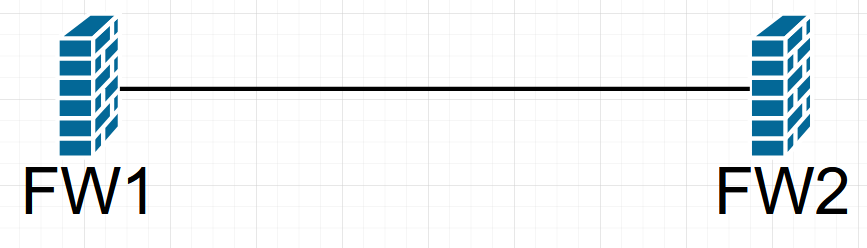
\includegraphics[width=0.6\textwidth,interpolate=false]{figures/firewall_vrrp.png}
     \caption{Firewalls VRRP}
   \label{fig:firewalls-vrrp}
 \end{figure}

\section{MLAG Design}
All switch pairs (ToRs and EoRs) are configured with MLAG setup.\\
- \textbf{Active-standby operation:} One switch forwards traffic while the standby remains ready; on failure, the standby takes over.\\
- \textbf{Sub-second \hyperref[def:failover]{\underline{failover:}}} If the active switch fails, traffic continues through the standby with minimal interruption.

% IMAGE: media/image11.png - MLAG diagram
 \begin{figure}[H]
    \centering
   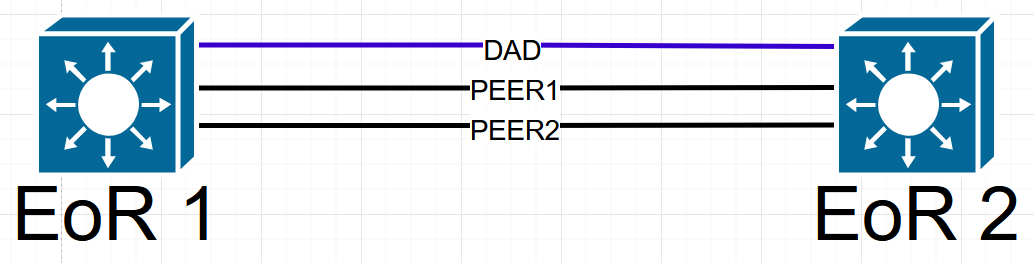
\includegraphics[width=0.6\textwidth,interpolate=false]{figures/eor_mlag.png}
   \caption{EoRs Pair MLAG Architecture}
   \label{fig:mlag}
\end{figure}

\section{Firewall Rules}
Firewall policies enforce strict zone isolation with default-deny rules. Traffic from Untrust to DMZ is permitted only for HTTP and HTTPS. Traffic from DMZ to Trust is permitted only for application-specific ports. All other cross-zone traffic is denied by default. Trust-zone outbound traffic to the external network is permitted via NAT. Management access to all devices is restricted to SSH only.

\section{Conclusion}
This chapter presented a complete spine-leaf data center design with two spines, eight leaves, full-mesh connectivity, and MLAG active-standby pairs at the ToR and EoR layers. Zone-based security separates DMZ, Trust, and Untrust zones via firewall policies, while VRRP supports 99.99\% availability targets.
\chapter{Implementation and Simulation}

\section{Introduction}
This chapter implements and validates the data center design from Chapter 2, translating the spine-leaf topology, VLANs, IP addressing, and redundancy into a working simulation. Challenges and their resolutions are documented below.
\section{Environment}
\subsection{Initial Tool Selection}
\begin{itemize}[nosep]
    \item Planned stack: Huawei eNSP\cite{ensp} + VirtualBox\cite{virtualbox} for servers.
    \item Failure: VirtualBox 5.2.44 crashes on Windows 11; eNSP reached end of life in 2022; Hyper-V conflict.
\end{itemize}
\subsection{Migration to VMware and PNETLab}
\begin{itemize}[nosep]
    \item VMware Workstation Pro 17\cite{vmware} + PNETLab 5.1\cite{pnetlab} + PuTTY\cite{putty} + Linux Debian servers.
    \item Resolved compatibility and multi-NIC requirements.
\end{itemize}
\subsection{Device Image Issues with Huawei CE12800}
\begin{itemize}[nosep]
    \item Unstable boot, 4 ports by default, high RAM (8\,GB+), no MLAG on available image.
\end{itemize}
\subsection{Switch to Arista vEOS}
\hyperref[def:veos]{\underline{Arista vEOS}}: reliable start, 24 ports, 2\,GB RAM, VLANs, trunks, VRRP, and MLAG. All spine and leaf switches were recreated.

\section{Device Configurations}

\subsection{PNETLab interface naming (Arista vEOS)}
Arista vEOS in PNETLab allows only Ethernet interfaces, while the LLD uses different ports. To overcome this challenge, we used the following port mapping in PNETLab:

\begin{table}[htbp]
    \centering
    \small
    \caption{PNETLab (Arista vEOS) to LLD port mapping.}
    \label{tab:pnetlab-port-map}
    \begin{tabular}{|l|l|l|}
        \hline
        \textbf{Switch} & \textbf{LLD interface(s)} & \textbf{PNETLab interface(s)} \\
        \hline
        ToR & \texttt{Ethernet0/0/1}--\texttt{Ethernet0/0/4} & \texttt{Eth1}--\texttt{Eth4} \\
        ToR & \texttt{GigabitEthernet0/0/1}--\texttt{GigabitEthernet0/0/5} & \texttt{Eth5}--\texttt{Eth9} \\
        EoR & \texttt{GigabitEthernet0/0/X} & \texttt{EthX} \\
        \hline
    \end{tabular}
\end{table}

\subsection{Spine switch (EoR-1)}
On EoR-1 we configured: VLANs 110, 120, 130, 210, 220; trunk Port-Channels (Po3--Po10) to all ToR switches; MLAG peer-link Po1 and firewall trunks Po20/Po30; management SVI 10.10.10.208/24 on VLAN~110; MLAG domain \texttt{MLAG-EOR} with peer 10.10.10.209. EoR-2 is configured identically to EoR-1; the only difference is MLAG priority, with EoR-2 operating as the secondary peer. Verification screenshots: Appendix~\ref{app:config-verify}, Figures~\ref{fig:app-eor1-vlans}--\ref{fig:app-eor1-mlag}.

\subsection{Leaf switch (ToR A-1)}
On ToR A-1 we configured: VLANs 110--220; server Port-Channels Po2--Po5 (mgmt/service bonds); uplink Po6 to both EoRs; MLAG peer-link Po1; management 10.10.10.200/24; MLAG domain \texttt{MLAG-TORA} with peer 10.10.10.201. ToR A-2 is configured identically to ToR A-1; the only difference is MLAG priority, with ToR A-2 operating as the secondary peer. Verification: Appendix~\ref{app:config-verify}, Figures~\ref{fig:app-tora1-vlans}--\ref{fig:app-tora1-mlag}.

\subsection{Firewalls (FW-1 and FW-2)}
On FW-1/FW-2 we configured: VLAN sub-interfaces on \texttt{lagg0} (110--220); per-zone IPs (e.g.\ 10.10.10.210 on FW-1); CARP virtual gateways (.254) on all VLANs; zone-based rules (DMZ/Trust separation, default deny). FW-1 master, FW-2 backup. Verification: Appendix~\ref{app:config-verify}, Figures~\ref{fig:app-fw1-vlans}--\ref{fig:app-fw1-rules}.

\subsection{Server (Server 1)}
On Server~1 we configured: \texttt{bond0} 10.10.10.1/24 (mgmt, eth0+eth2); \texttt{bond1} 10.10.20.1/24 (service, eth1+eth3). Servers~2 through~8 are configured identically; only the management and service IP addresses differ according to the LLD. Verification: Appendix~\ref{app:config-verify}, Figure~\ref{fig:app-server1-config}.

\section{Connectivity Testing}

After all devices were configured, ICMP ping tests were executed between Linux servers to validate end-to-end connectivity. Table~\ref{tab:ping-tests} lists every test with its scope (intra/inter cabinet, VLAN, management or service plane, and security zone) and the observed result. Terminal screenshots are provided in Appendix~\ref{app:tests}.

\begin{table}[htbp]
    \centering
    \small
    \caption{Server-to-server ping test results}
    \label{tab:ping-tests}
    \begin{tabular}{|l|l|c|c|c|c|c|}
        \hline
        \textbf{Source} & \textbf{Destination} & \textbf{Cabinet} & \textbf{VLAN} & \textbf{Plane} & \textbf{Zone} & \textbf{Result} \\
        \hline
        Server~1 & Server~2 (10.10.10.2) & A & 110 & Mgmt & Trust & ALLOWED \\
        \hline
        Server~1 & Server~2 (10.10.20.2) & A & 120 & Service & Trust & ALLOWED \\
        \hline
        Server~1 & Server~3 (10.10.20.3) & A--B & 120 & Service & Trust & ALLOWED \\
        \hline
        Server~1 & Server~5 (10.10.30.1) & A--C & 120--130 & Service & Trust & ALLOWED \\
        \hline
        Server~7 & Server~8 (10.20.20.2) & D & 220 & Service & DMZ & ALLOWED \\
        \hline
        Server~1 & Server~7 (10.20.10.1) & A--D & 110--210 & Mgmt & Trust--DMZ & ALLOWED \\
        \hline
        Server~7 & Server~1 (10.10.10.1) & D--A & 210--110 & Mgmt & DMZ--Trust & BLOCKED \\
        \hline
    \end{tabular}
\end{table}

All \texttt{ALLOWED} flows completed successfully, confirming correct VLAN assignment, inter-VLAN routing on the EoR switches, and server bonding. The single \texttt{BLOCKED} test (DMZ--Trust management) validates zone-based firewall policy. Together, the tests cover intra- and inter-cabinet paths, management and service planes, and both intra-zone and inter-zone traffic.

\section{Redundancy \& Failure Testing}

Redundancy was validated by shutting down the active node in each redundant pair and verifying that the standby assumed control. Firewall and EoR pairs were each tested once. At the leaf layer, all four ToR pairs (Cabinets A--D) use the same MLAG active-standby design; the ToR~B test below is documented as representative, because the failover procedure and expected outcome are identical for every cabinet pair.

\subsection{VRRP (CARP) firewall failover test}
\begin{itemize}[nosep]
    \item Stop FW-1; keep pings to CARP gateway addresses.
    \item Observe FW-2 \texttt{MASTER} on all VLANs (Figure~\ref{fig:redund-fw2}).
    \item Result: active-standby firewall failover confirmed.
\end{itemize}
\begin{figure}[htbp]
    \centering
    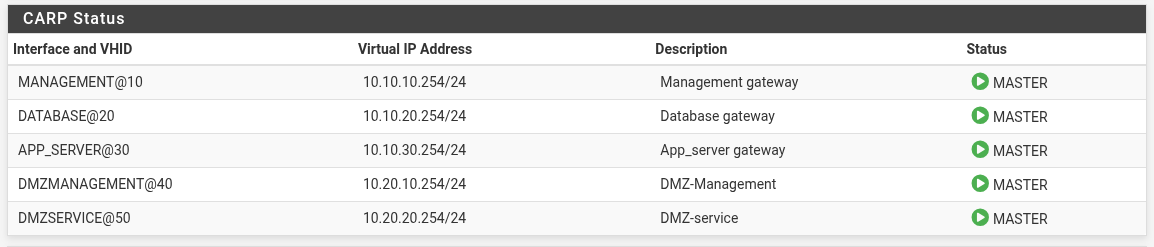
\includegraphics[width=0.72\textwidth,interpolate=false]{figures/redundancy_tests/fw2_after_failover.png}
    \caption{VRRP (CARP) on FW-2 after FW-1 failure.}
    \label{fig:redund-fw2}
\end{figure}

\subsection{EoR MLAG failover test}
\begin{itemize}[nosep]
    \item Shut down EoR-1; run \texttt{show mlag detail} on EoR-2.
    \item Observe \texttt{Failover: True}, cause \texttt{Peer Link Down} (Figure~\ref{fig:redund-eor2}).
    \item Result: backup spine continues forwarding.
\end{itemize}
\begin{figure}[htbp]
    \centering
    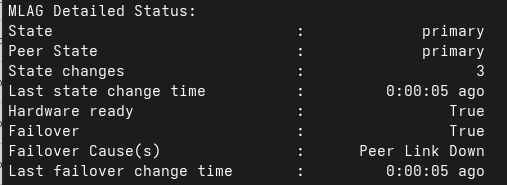
\includegraphics[width=0.65\textwidth,interpolate=false]{figures/redundancy_tests/eor2_after_failover.png}
    \caption{MLAG status on EoR-2 after EoR-1 failure.}
    \label{fig:redund-eor2}
\end{figure}

\subsection{ToR B MLAG failover test}
\begin{itemize}[nosep]
    \item Shut down ToR B-1 with traffic on Cabinet~B servers.
    \item Observe ToR B-2 MLAG primary after peer-link loss (Figure~\ref{fig:redund-torb2}).
    \item Result: leaf active-standby recovery confirmed.
\end{itemize}
\begin{figure}[htbp]
    \centering
    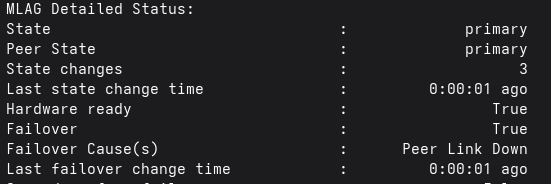
\includegraphics[width=0.65\textwidth,interpolate=false]{figures/redundancy_tests/torb2_after_failover.png}
    \caption{MLAG status on ToR B-2 after ToR B-1 failure.}
    \label{fig:redund-torb2}
\end{figure}

\section{Simulation Environment Status}

% IMAGE: media/image15.png - PNETLab environment screenshot
% \begin{figure}[H]
%     \centering
%     \includegraphics[width=0.9\textwidth]{figures/pnetlab-environment.png}
%     \caption{PNETLab simulation environment showing full topology}
%     \label{fig:pnetlab-env}
% \end{figure}

The final simulation environment runs on:

\begin{itemize}[nosep,itemsep=0pt,topsep=2pt,parsep=0pt,partopsep=0pt]
    \item \textbf{Host:} Windows 11 Pro with VMware Workstation Pro 17
    \item \textbf{PNETLab VM:} 10 vCPUs, 24GB RAM, 100GB storage
    \item \textbf{Total device count:}
    \begin{itemize}[nosep,itemsep=0pt,topsep=0pt,parsep=0pt,partopsep=0pt,leftmargin=1.5em]
        \item 2 spine switches (Arista vEOS)
        \item 8 leaf switches (Arista vEOS)
        \item 2 firewalls (pfSense)
        \item 8 servers (Linux Debian)
    \end{itemize}
    \item \textbf{Resource utilization:} 30\% CPU, 70\% RAM
\end{itemize}

All devices start reliably and maintain stable connections.

\section{Conclusion}
This chapter has presented the complete implementation and validation of the data center design. 
The implemented data center provides a solid foundation for client application deployment, with configuration verification in Appendix~E, connectivity tests in Appendix~D, and LLD tables in Appendix~B.
\chapter*{General Conclusion}
\addcontentsline{toc}{chapter}{General Conclusion}

This dissertation addressed the design and simulation of a modern data center network architecture using spine-leaf topology with full mesh redundancy, active-standby MLAG operation, and zone-based security. The work was structured into three complementary chapters. Chapter 1 established the theoretical foundations, comparing traditional three-tier architecture with modern spine-leaf. Chapter 2 translated these concepts into a concrete design comprising four cabinets, eight ToR leaf switches, two EoR spine switches, and two firewalls in full mesh topology, with five VLANs across Trust and DMZ zones. Chapter 3 implemented the complete design in simulation, migrating from eNSP to PNETLab, from Huawei CE12800 to Arista vEOS, and from VPCS to Linux servers.\\
The principal achievements of this project are: a complete spine-leaf implementation with 2 spines, 8 leaves, 16 paths, and full mesh connectivity; active-standby redundancy at the ToR, EoR, and firewall layers (\hyperref[def:activestandby]{\underline{active-standby}} with VRRP/MLAG) providing sub-second failover; zone-based security ensuring that web layer compromise cannot propagate to database servers; comprehensive validation through five failure scenarios (spine failure, leaf failure, link failure, NIC failure, and cabinet failure); professional documentation including HLD, LLD, UML diagrams, configuration templates, and test results; and thorough problem-solving documentation of the migration from incompatible tools.\\
Despite these achievements, several limitations remain. Complete cabinet failure isolates all servers in that cabinet; true high availability would require cross-cabinet replication. Storage networking (SAN/NAS) was not implemented, and the design remains simulated rather than deployed on physical hardware. These limitations inform future work directions.\\
In conclusion, this project successfully demonstrates a production-ready, carrier-grade data center blueprint that is validated, documented, and ready for enterprise deployment.

% Back matter after conclusion: no page numbers (conclusion stays the last numbered page)
\pagenumbering{gobble}
\appendix
\chapter{DEFINITIONS}
\label{app:definitions}

\section*{A.1 Network Architecture Definitions}
\addcontentsline{toc}{section}{A.1 Network Architecture Definitions}

\subsection*{Spine Switch}
\label{def:spine}
A \textbf{spine switch} forms the core forwarding layer in spine-leaf architecture. 
It connects only to leaf switches (no direct server connections) and operates 
at Layer 3 for routing between leaf switches. In our design, EoR-1 and EoR-2 
serve as spine switches.

\subsection*{Leaf Switch (ToR)}
\label{def:leaf}
A \textbf{leaf switch} (Top of Rack) provides server connectivity in the access 
layer. It connects to servers via access ports and uplinks to all spine switches 
via trunk ports. In our design, we have eight leaf switches (ToR A-1 through 
ToR D-2).

\subsection*{Spine-Leaf Architecture}
\label{def:spineleaf}
\textbf{Spine-Leaf architecture} is a two-tier network topology where every 
leaf switch connects to every spine switch in a full mesh. Any server reaches 
any other server in exactly two hops, providing consistent latency and ECMP 
load balancing.

\subsection*{Three-Tier Architecture}
\label{def:threetier}
\textbf{Three-Tier architecture} is a traditional data center architecture 
consisting of core layer (backbone), aggregation layer (policy enforcement), 
and access layer (server connectivity). Designed for north-south traffic.

\subsection*{EoR (End of Row)}
\label{def:eor}
An \textbf{End-of-Row switch} is placed at the end of a row of server racks, 
connecting all servers in that row. In our design, EoR-1 and EoR-2 function as 
spine switches.

\subsection*{ToR (Top of Rack)}
\label{def:tor}
A \textbf{Top-of-Rack switch} is located at the top of a server cabinet, 
connecting all servers within that cabinet. In our design, we have eight 
ToR switches (two per cabinet).

\subsection*{Full Mesh}
\label{def:fullmesh}
\textbf{Full mesh} is a topology where every device connects directly to every 
other device. In spine-leaf architecture, every leaf switch connects to every 
spine switch.
\subsection*{Cluster}
\label{def:cluster}
A \textbf{cluster} is a group of physical servers that act as a single 
logical unit to provide high availability and load balancing. In our 
project, one Linux instance represents a cluster of four physical servers.

\section*{A.2 VLAN and Switching Definitions}
\addcontentsline{toc}{section}{A.2 VLAN and Switching Definitions}

\subsection*{VLAN (Virtual Local Area Network)}
\label{def:vlan}
A \textbf{VLAN} is a logical subdivision of a physical network that groups 
devices based on function or security requirements rather than physical 
location. VLANs isolate traffic, reduce broadcast domains, and improve 
security.

\subsection*{Trunk Port}
\label{def:trunk}
A \textbf{trunk port} is a switch port that carries traffic for multiple 
VLANs simultaneously using 802.1Q tagging. Used for inter-switch connections.

\subsection*{Access Port}
\label{def:accessport}
An \textbf{access port} is a switch port that belongs to a single VLAN and 
carries untagged traffic. Used for connecting end devices like servers.

\section*{A.3 Redundancy and High Availability Definitions}
\addcontentsline{toc}{section}{A.3 Redundancy and High Availability Definitions}

\subsection*{VRRP (Virtual Router Redundancy Protocol)}
\label{def:vrrp}
\textbf{VRRP} is a protocol that allows multiple routers to share a single 
virtual IP address. If the master router fails, a backup takes over 
automatically within seconds, providing gateway redundancy.

\subsection*{MLAG (Multi-Chassis Link Aggregation)}
\label{def:mlag}
\textbf{MLAG} is a technology that allows two physical switches to appear as 
a single logical switch to connected devices. In our design, MLAG pairs operate 
in active-standby mode with master/backup switches.

\subsection*{Active-Active}
\label{def:activeactive}
\textbf{Active-active} is an alternative redundancy mode where both devices forward traffic 
simultaneously. This mode is not used in our design.

\subsection*{Active-Standby}
\label{def:activestandby}
\textbf{Active-standby} is a redundancy mode where one device (master) handles 
all traffic while the other (standby) remains idle until the master fails. 
VRRP uses this mode for gateways and firewalls. MLAG pairs at the ToR and EoR 
layers also operate in active-standby mode in our design.

\subsection*{Failover}
\label{def:failover}
\textbf{Failover} is the automatic switching from a failed primary component 
to a redundant backup component.

\section*{A.4 Security Definitions}
\addcontentsline{toc}{section}{A.4 Security Definitions}

\subsection*{DMZ (Demilitarized Zone)}
\label{def:dmz}
\textbf{DMZ} is a semi-trusted zone for public-facing services such as web 
servers. It sits between the internet (untrust) and the internal network 
(trust). Accessible from internet on specific ports (HTTP/HTTPS).

\subsection*{Trust Zone}
\label{def:trust}
The \textbf{Trust zone} is the most secure zone for internal services including 
application servers, database servers, and management networks. No direct 
internet access.

\subsection*{Untrust Zone}
\label{def:untrust}
The \textbf{Untrust zone} represents all external networks (internet) and is 
considered completely untrusted. All traffic must pass through firewall 
inspection.

\subsection*{Firewall}
\label{def:firewall}
A \textbf{firewall} is a security device that inspects and filters network 
traffic based on configured rules. Enforces zone-based security policies and 
performs stateful packet inspection.

\subsection*{NAT (Network Address Translation)}
\label{def:nat}
\textbf{NAT} is a method that maps private IP addresses to public IP addresses, 
allowing internal devices to communicate with the internet while hiding 
internal network structure.

\section*{A.5 Virtualization Definitions}
\addcontentsline{toc}{section}{A.5 Virtualization Definitions}

\subsection*{Hypervisor}
\label{def:hypervisor}
A \textbf{hypervisor} is software that creates and runs virtual machines by 
abstracting the underlying physical hardware (e.g., VMware ESXi).

\subsection*{Virtual Machine (VM)}
\label{def:vm}
A \textbf{virtual machine} is an emulation of a computer system that runs its 
own operating system on top of a hypervisor.

\subsection*{Server Cluster}
\label{def:servercluster}
A \textbf{server cluster} is a group of physical servers that act as a single 
logical unit for high availability and load balancing. In our project, one 
Linux instance represents a cluster.

\subsection*{VMware}
\label{def:vmware}
\textbf{VMware} is a virtualization platform that allows running multiple 
virtual machines on a single physical server.

\section*{A.6 Simulation and Tools Definitions}
\addcontentsline{toc}{section}{A.6 Simulation and Tools Definitions}

\subsection*{eNSP (Enterprise Network Simulation Platform)}
\label{def:ensp}
\textbf{eNSP} is Huawei's official network simulation platform for designing 
and testing networks without physical hardware. Requires VirtualBox 5.2.44.

\subsection*{PNETLab (Practical Networking Lab)}
\label{def:pnetlab}
\textbf{PNETLab} is a community-maintained network simulation platform 
(EVE-NG fork) that runs on VMware and supports multiple device images 
(Arista vEOS, Debian Linux, Huawei CE12800).

\subsection*{Arista vEOS}
\label{def:veos}
\textbf{Arista vEOS} (Virtual Extensible Operating System) is Arista's virtual 
network device emulator used in our project for spine and leaf switches. 
Supports VLANs, trunk ports, VRRP, OSPF, and MLAG with 2GB RAM per instance.

\subsection*{VMware Workstation Pro}
\label{def:vmwareworkstation}
\textbf{VMware Workstation Pro} is a Type-2 hypervisor used to host the 
PNETLab virtual machine, providing hardware virtualization support.

\subsection*{PuTTY}
\label{def:putty}
\textbf{PuTTY} is a free SSH and Telnet client used in our project to access 
network devices and servers for configuration and testing.

\subsection*{VPCS (Virtual PC Simulator)}
\label{def:vpcs}
\textbf{VPCS} is a lightweight tool included with PNETLab that simulates a 
simple PC. Limited to one IP address per device, replaced by Linux Tiny Core.

\section*{A.7 Server and Network Interface Definitions}
\addcontentsline{toc}{section}{A.7 Server and Network Interface Definitions}

\subsection*{NIC (Network Interface Card)}
\label{def:nic}
A \textbf{NIC} (Network Interface Card) is a hardware component that connects 
a server to a network. In our design, each server has four NICs (M1, M2, S1, S2).

\subsection*{Management Network (M1/M2)}
\label{def:management}
The \textbf{management network} is the network interface used by administrators 
to access servers for configuration, monitoring, and maintenance. Isolated 
from service traffic.

\subsection*{Service Network (S1/S2)}
\label{def:service}
The \textbf{service network} is the network interface used for application 
traffic between servers (web to app, app to database). Separate from 
management network for security.

\section*{A.8 Documentation Definitions}
\addcontentsline{toc}{section}{A.8 Documentation Definitions}

\subsection*{HLD (High-Level Design)}
\label{def:hld}
\textbf{HLD} (High-Level Design) is a top-level design document showing the 
overall architecture, major components, and their relationships without 
implementation details.

\subsection*{LLD (Low-Level Design)}
\label{def:lld}
\textbf{LLD} (Low-Level Design) is a detailed design document containing 
specific IP addresses, VLAN assignments, port connections, configuration 
commands, and implementation procedures.

\subsection*{UML (Unified Modeling Language)}
\label{def:uml}
\textbf{UML} (Unified Modeling Language) is a standardized modeling language 
used to visualize system design. In our project, we used use case diagrams 
and sequence diagrams.

\subsection*{Use Case Diagram}
\label{def:usecase}
A \textbf{use case diagram} is a UML diagram showing actors (users or systems) 
and their interactions with the system. Used to identify functional 
requirements.

\subsection*{Sequence Diagram}
\label{def:sequence}
A \textbf{sequence diagram} is a UML diagram showing the temporal order of 
message exchanges between objects. Used to illustrate operational flows and 
failure scenarios.
\chapter{Appendix B: Low-Level Design (LLD)}
\label{app:lld}

\section{Device inventory}
\addcontentsline{toc}{section}{B.1 Device inventory}

\begin{figure}[H]
    \centering
    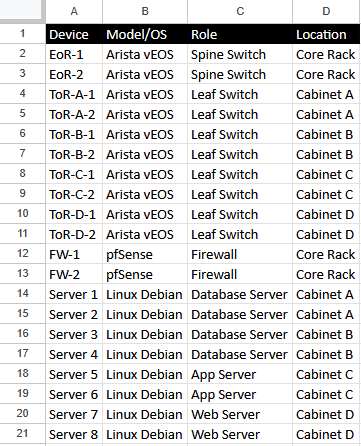
\includegraphics[width=0.65\textwidth,height=0.68\textheight,keepaspectratio]{figures/device_inventory.png}
    \caption{Complete device inventory (LLD).}
    \label{fig:app-device-inventory}
\end{figure}

\section{IP addressing plan}
\addcontentsline{toc}{section}{B.2 IP addressing plan}
\thispagestyle{plain}
\begingroup
\let\clearpage\relax
\begin{sidewaysfigure}[p]
    \centering
    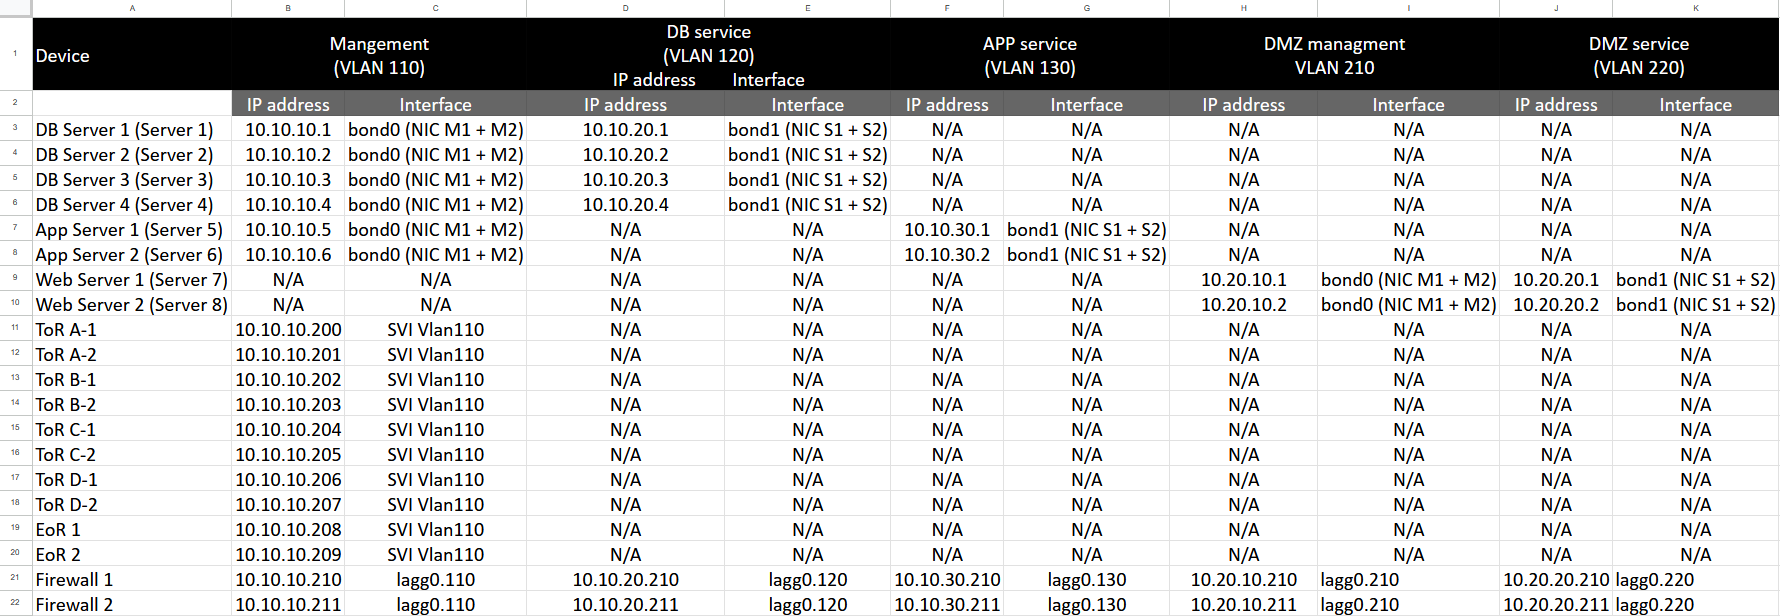
\includegraphics[width=1\textheight,keepaspectratio]{figures/ip.png}
    \caption{Complete IP addressing plan (LLD).}
    \label{fig:app-ip-plan}
\end{sidewaysfigure}
\endgroup
\clearpage

\section{Physical port connections}
\addcontentsline{toc}{section}{B.3 Physical port connections}

\begin{figure}[H]
    \centering
    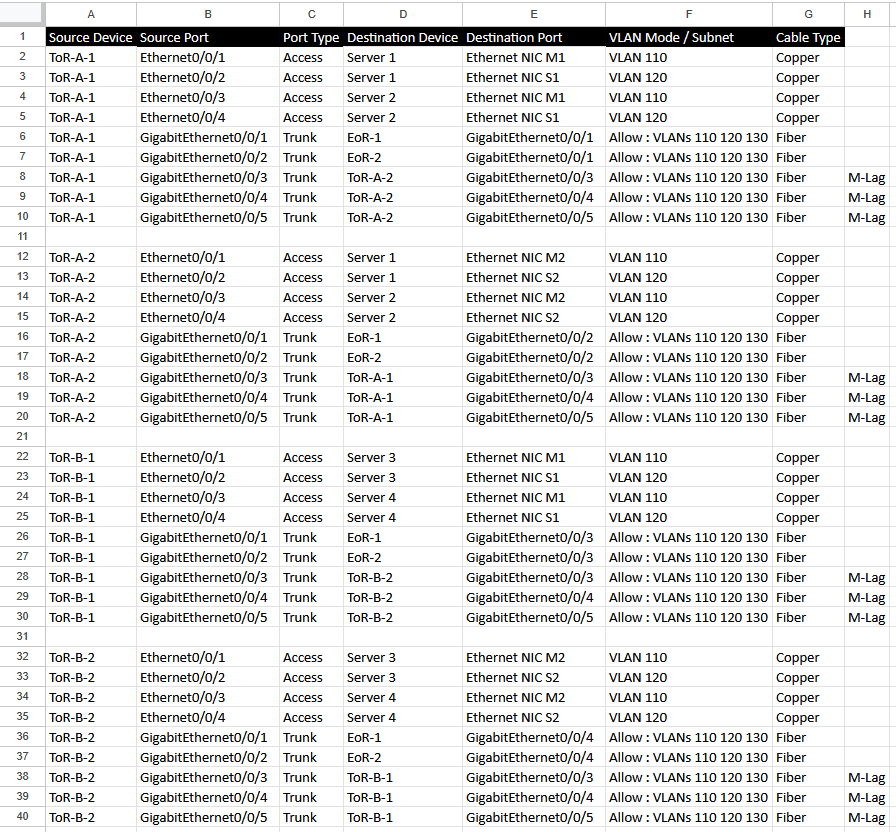
\includegraphics[width=\textwidth,keepaspectratio]{figures/port_connections/port_connections_1.png}
    \caption{Port connections matrix (part 1).}
    \label{fig:app-port-conn-1}
\end{figure}

\begin{figure}[H]
    \centering
    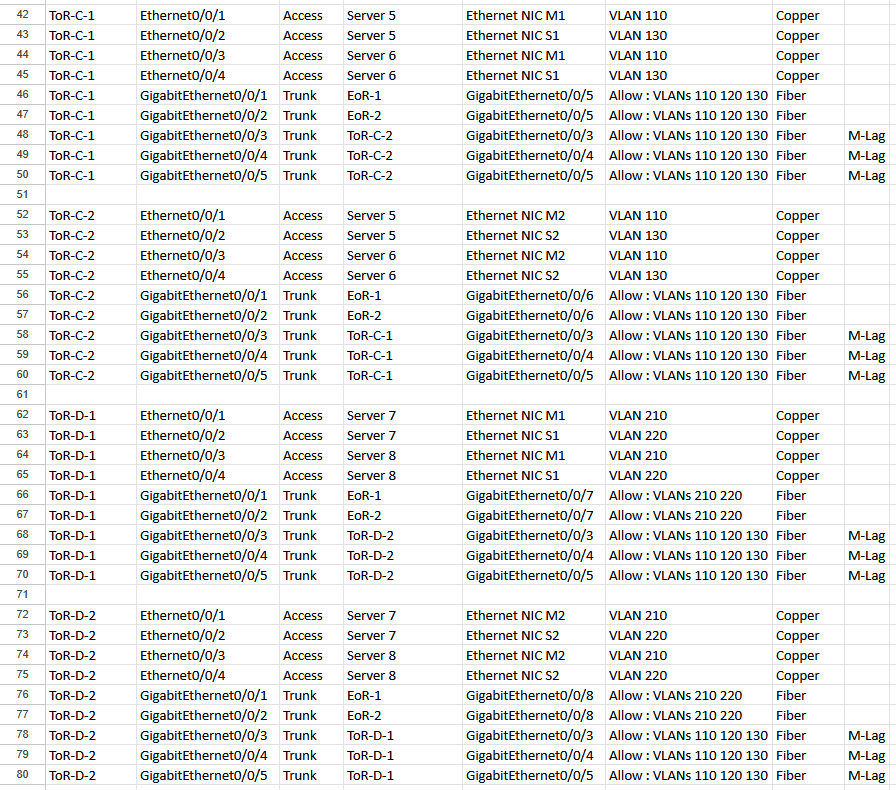
\includegraphics[width=\textwidth,keepaspectratio]{figures/port_connections/port_connections_2.png}
    \caption{Port connections matrix (part 2).}
    \label{fig:app-port-conn-2}
\end{figure}

\begin{figure}[H]
    \centering
    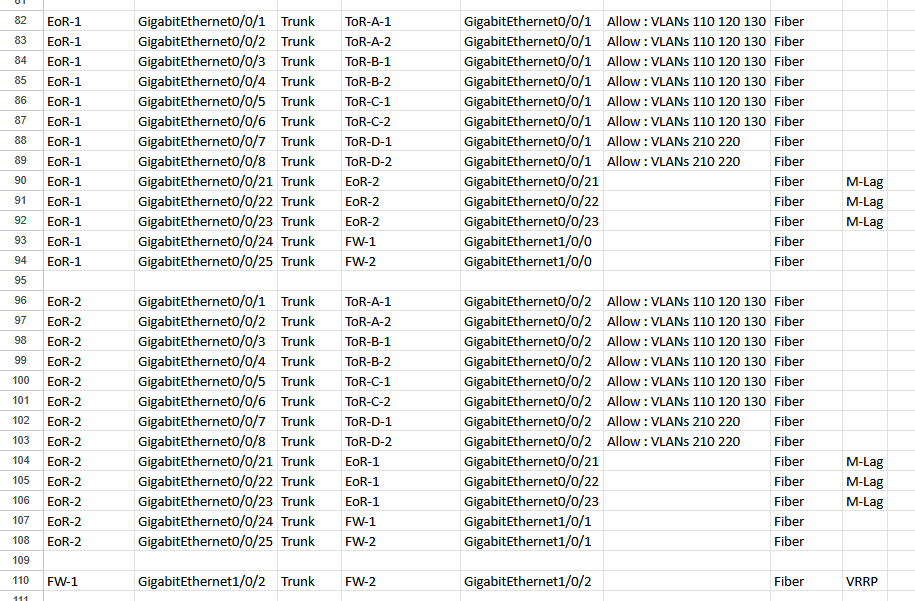
\includegraphics[width=\textwidth,keepaspectratio]{figures/port_connections/port_connections_3.png}
    \caption{Port connections matrix (part 3).}
    \label{fig:app-port-conn-3}
\end{figure}

% Appendix C: server network configuration scripts
\chapter{Appendix C: Device Configurations and Scripts}
\label{app:configs}

\section{Server network configurations}
\addcontentsline{toc}{section}{C.1 Server network configurations}

The following listings show the \texttt{/etc/network/interfaces} configuration applied on each Linux server (Servers~1--8), in cabinet order.

\subsection{Server 1}
\addcontentsline{toc}{section}{C.1.1 Server 1}
\begin{lstlisting}[caption={Server 1: network interfaces (Cabinet A).},basicstyle=\ttfamily\footnotesize,breaklines=true]
source /etc/network/interfaces.d/*

auto lo
iface lo inet loopback

allow-hotplug eth0
iface eth0 inet manual

allow-hotplug eth1
iface eth1 inet manual

allow-hotplug eth2
iface eth2 inet manual

allow-hotplug eth3
iface eth3 inet manual

auto bond0
iface bond0 inet static
    address 10.10.10.1
    netmask 255.255.255.0
    gateway 10.10.10.254
    bond-slaves eth0 eth2
    bond-mode active-backup
    bond-miimon 100
    bond-updelay 200
    bond-downdelay 200

auto bond1
iface bond1 inet static
    address 10.10.20.1
    netmask 255.255.255.0
    bond-slaves eth1 eth3
    bond-mode active-backup
    bond-miimon 100
    bond-updelay 200
    bond-downdelay 200
\end{lstlisting}

\subsection{Server 2}
\addcontentsline{toc}{section}{C.1.2 Server 2}
\begin{lstlisting}[caption={Server 2: network interfaces (Cabinet A).},basicstyle=\ttfamily\footnotesize,breaklines=true]
source /etc/network/interfaces.d/*

auto lo
iface lo inet loopback

allow-hotplug eth0
iface eth0 inet manual

allow-hotplug eth1
iface eth1 inet manual

allow-hotplug eth2
iface eth2 inet manual

allow-hotplug eth3
iface eth3 inet manual

auto bond0
iface bond0 inet static
    address 10.10.10.2
    netmask 255.255.255.0
    gateway 10.10.10.254
    bond-slaves eth0 eth2
    bond-mode active-backup
    bond-miimon 100
    bond-updelay 200
    bond-downdelay 200

auto bond1
iface bond1 inet static
    address 10.10.20.2
    netmask 255.255.255.0
    bond-slaves eth1 eth3
    bond-mode active-backup
    bond-miimon 100
    bond-updelay 200
    bond-downdelay 200
\end{lstlisting}

\subsection{Server 3}
\addcontentsline{toc}{section}{C.1.3 Server 3}
\begin{lstlisting}[caption={Server 3: network interfaces (Cabinet B).},basicstyle=\ttfamily\footnotesize,breaklines=true]
source /etc/network/interfaces.d/*

auto lo
iface lo inet loopback

allow-hotplug eth0
iface eth0 inet manual

allow-hotplug eth1
iface eth1 inet manual

allow-hotplug eth2
iface eth2 inet manual

allow-hotplug eth3
iface eth3 inet manual

auto bond0
iface bond0 inet static
    address 10.10.10.3
    netmask 255.255.255.0
    gateway 10.10.10.254
    bond-slaves eth0 eth2
    bond-mode active-backup
    bond-miimon 100
    bond-updelay 200
    bond-downdelay 200

auto bond1
iface bond1 inet static
    address 10.10.20.3
    netmask 255.255.255.0
    bond-slaves eth1 eth3
    bond-mode active-backup
    bond-miimon 100
    bond-updelay 200
    bond-downdelay 200
\end{lstlisting}

\subsection{Server 4}
\addcontentsline{toc}{section}{C.1.4 Server 4}
\begin{lstlisting}[caption={Server 4: network interfaces (Cabinet B).},basicstyle=\ttfamily\footnotesize,breaklines=true]
source /etc/network/interfaces.d/*

auto lo
iface lo inet loopback

allow-hotplug eth0
iface eth0 inet manual

allow-hotplug eth1
iface eth1 inet manual

allow-hotplug eth2
iface eth2 inet manual

allow-hotplug eth3
iface eth3 inet manual

auto bond0
iface bond0 inet static
    address 10.10.10.4
    netmask 255.255.255.0
    gateway 10.10.10.254
    bond-slaves eth0 eth2
    bond-mode active-backup
    bond-miimon 100
    bond-updelay 200
    bond-downdelay 200

auto bond1
iface bond1 inet static
    address 10.10.20.4
    netmask 255.255.255.0
    bond-slaves eth1 eth3
    bond-mode active-backup
    bond-miimon 100
    bond-updelay 200
    bond-downdelay 200
\end{lstlisting}

\subsection{Server 5}
\addcontentsline{toc}{section}{C.1.5 Server 5}
\begin{lstlisting}[caption={Server 5: network interfaces (Cabinet C).},basicstyle=\ttfamily\footnotesize,breaklines=true]
source /etc/network/interfaces.d/*

auto lo
iface lo inet loopback

allow-hotplug eth0
iface eth0 inet manual

allow-hotplug eth1
iface eth1 inet manual

allow-hotplug eth2
iface eth2 inet manual

allow-hotplug eth3
iface eth3 inet manual

auto bond0
iface bond0 inet static
    address 10.10.10.5
    netmask 255.255.255.0
    gateway 10.10.10.254
    bond-slaves eth0 eth2
    bond-mode active-backup
    bond-miimon 100
    bond-updelay 200
    bond-downdelay 200

auto bond1
iface bond1 inet static
    address 10.10.30.1
    netmask 255.255.255.0
    bond-slaves eth1 eth3
    bond-mode active-backup
    bond-miimon 100
    bond-updelay 200
    bond-downdelay 200
\end{lstlisting}

\subsection{Server 6}
\addcontentsline{toc}{section}{C.1.6 Server 6}
\begin{lstlisting}[caption={Server 6: network interfaces (Cabinet C).},basicstyle=\ttfamily\footnotesize,breaklines=true]
source /etc/network/interfaces.d/*

auto lo
iface lo inet loopback

allow-hotplug eth0
iface eth0 inet manual

allow-hotplug eth1
iface eth1 inet manual

allow-hotplug eth2
iface eth2 inet manual

allow-hotplug eth3
iface eth3 inet manual

auto bond0
iface bond0 inet static
    address 10.10.10.6
    netmask 255.255.255.0
    gateway 10.10.10.254
    bond-slaves eth0 eth2
    bond-mode active-backup
    bond-miimon 100
    bond-updelay 200
    bond-downdelay 200

auto bond1
iface bond1 inet static
    address 10.10.30.2
    netmask 255.255.255.0
    bond-slaves eth1 eth3
    bond-mode active-backup
    bond-miimon 100
    bond-updelay 200
    bond-downdelay 200
\end{lstlisting}

\subsection{Server 7}
\addcontentsline{toc}{section}{C.1.7 Server 7}
\begin{lstlisting}[caption={Server 7: network interfaces (Cabinet D, DMZ).},basicstyle=\ttfamily\footnotesize,breaklines=true]
source /etc/network/interfaces.d/*

auto lo
iface lo inet loopback

allow-hotplug eth0
iface eth0 inet manual

allow-hotplug eth1
iface eth1 inet manual

allow-hotplug eth2
iface eth2 inet manual

allow-hotplug eth3
iface eth3 inet manual

auto bond0
iface bond0 inet static
    address 10.20.10.1
    netmask 255.255.255.0
    gateway 10.20.10.254
    bond-slaves eth0 eth2
    bond-mode active-backup
    bond-miimon 100
    bond-updelay 200
    bond-downdelay 200

auto bond1
iface bond1 inet static
    address 10.20.20.1
    netmask 255.255.255.0
    bond-slaves eth1 eth3
    bond-mode active-backup
    bond-miimon 100
    bond-updelay 200
    bond-downdelay 200
\end{lstlisting}

\subsection{Server 8}
\addcontentsline{toc}{section}{C.1.8 Server 8}
\begin{lstlisting}[caption={Server 8: network interfaces (Cabinet D, DMZ).},basicstyle=\ttfamily\footnotesize,breaklines=true]
source /etc/network/interfaces.d/*

auto lo
iface lo inet loopback

allow-hotplug eth0
iface eth0 inet manual

allow-hotplug eth1
iface eth1 inet manual

allow-hotplug eth2
iface eth2 inet manual

allow-hotplug eth3
iface eth3 inet manual

auto bond0
iface bond0 inet static
    address 10.20.10.2
    netmask 255.255.255.0
    gateway 10.20.10.254
    bond-slaves eth0 eth2
    bond-mode active-backup
    bond-miimon 100
    bond-updelay 200
    bond-downdelay 200

auto bond1
iface bond1 inet static
    address 10.20.20.2
    netmask 255.255.255.0
    bond-slaves eth1 eth3
    bond-mode active-backup
    bond-miimon 100
    bond-updelay 200
    bond-downdelay 200
\end{lstlisting}

\section{Firewall configuration (FW-1 and FW-2)}
\addcontentsline{toc}{section}{C.2 Firewall configuration (FW-1 and FW-2)}

Both firewalls run pfSense and are configured identically except for their individual interface IPs. Configuration is performed through the pfSense web GUI and follows seven sequential phases.

\subsection{LAGG interface creation}
\addcontentsline{toc}{section}{C.2.1 LAGG interface creation}

Navigate to \texttt{Interfaces} $\rightarrow$ \texttt{LAGGs} $\rightarrow$ \texttt{Add} and configure the link aggregation group:

\begin{itemize}[nosep]
    \item Parent interfaces: \texttt{vtnet0} and \texttt{vtnet1}
    \item LAGG protocol: LACP
    \item LACP timeout: Slow
    \item Hash algorithm: Layer 2/3/4
    \item Description: \texttt{Uplink-to-EoR}
\end{itemize}

\subsection{VLAN creation}
\addcontentsline{toc}{section}{C.2.2 VLAN creation}

Navigate to \texttt{Interfaces} $\rightarrow$ \texttt{VLANs} $\rightarrow$ \texttt{Add} and create five VLAN sub-interfaces on \texttt{lagg0}:

\begin{table}[htbp]
    \centering
    \caption{VLAN sub-interfaces on \texttt{lagg0}.}
    \label{tab:fw-vlans}
    \begin{tabular}{|l|c|l|}
        \hline
        \textbf{Parent} & \textbf{VLAN tag} & \textbf{Description} \\
        \hline
        lagg0 & 110 & Management \\
        lagg0 & 120 & Database \\
        lagg0 & 130 & App \\
        lagg0 & 210 & DMZ-Management \\
        lagg0 & 220 & DMZ-Service \\
        \hline
    \end{tabular}
\end{table}

\subsection{Interface assignment}
\addcontentsline{toc}{section}{C.2.3 Interface assignment}

Navigate to \texttt{Interfaces} $\rightarrow$ \texttt{Interface Assignments} and add each sub-interface in order:

\begin{table}[htbp]
    \centering
    \caption{Firewall interface assignments.}
    \label{tab:fw-if-assign}
    \begin{tabular}{|l|l|}
        \hline
        \textbf{Sub-interface} & \textbf{Assigned name} \\
        \hline
        lagg0.110 & OPT1 \\
        lagg0.120 & OPT2 \\
        lagg0.130 & OPT3 \\
        lagg0.210 & OPT4 \\
        lagg0.220 & OPT5 \\
        vtnet2 & OPT6 \\
        \hline
    \end{tabular}
\end{table}

\subsection{Interface IP configuration}
\addcontentsline{toc}{section}{C.2.4 Interface IP configuration}

Navigate to \texttt{Interfaces} $\rightarrow$ \texttt{OPTx} for each interface and apply the following static IPv4 addresses. All interfaces are enabled with IPv4 configuration type set to Static.

\begin{table}[htbp]
    \centering
    \small
    \caption{Firewall interface IP addresses (FW-1 and FW-2).}
    \label{tab:fw-ips}
    \begin{tabular}{|l|l|c|c|}
        \hline
        \textbf{Interface} & \textbf{Description} & \textbf{FW-1 address} & \textbf{FW-2 address} \\
        \hline
        OPT1 (lagg0.110) & MGMT & 10.10.10.220/24 & 10.10.10.221/24 \\
        OPT2 (lagg0.120) & DATABASE & 10.10.20.220/24 & 10.10.20.221/24 \\
        OPT3 (lagg0.130) & APP\_SERVER & 10.10.30.220/24 & 10.10.30.221/24 \\
        OPT4 (lagg0.210) & DMZMANAGEMENT & 10.20.10.220/24 & 10.20.10.221/24 \\
        OPT5 (lagg0.220) & DMZSERVICE & 10.20.20.220/24 & 10.20.20.221/24 \\
        OPT6 (vtnet2) & PFSYNC & 10.254.1.1/30 & 10.254.1.2/30 \\
        \hline
    \end{tabular}
\end{table}

\subsection{CARP virtual IP creation}
\addcontentsline{toc}{section}{C.2.5 CARP virtual IP creation}

Navigate to \texttt{Firewall} $\rightarrow$ \texttt{Virtual IPs} $\rightarrow$ \texttt{Add} and create five CARP virtual IPs on FW-1 only. FW-2 receives them automatically via XMLRPC synchronization. All VIPs use the same virtual IP password for CARP advertisement.

\begin{table}[htbp]
    \centering
    \small
    \caption{CARP virtual gateway addresses (configured on FW-1).}
    \label{tab:fw-carp}
    \begin{tabular}{|l|c|c|c|l|}
        \hline
        \textbf{Interface} & \textbf{Type} & \textbf{Virtual address} & \textbf{VHID} & \textbf{Description} \\
        \hline
        MGMT & CARP & 10.10.10.254/24 & 10 & Management gateway \\
        DATABASE & CARP & 10.10.20.254/24 & 20 & Database gateway \\
        APP\_SERVER & CARP & 10.10.30.254/24 & 30 & App gateway \\
        DMZMANAGEMENT & CARP & 10.20.10.254/24 & 40 & DMZ-Mgmt gateway \\
        DMZSERVICE & CARP & 10.20.20.254/24 & 50 & DMZ-Service gateway \\
        \hline
    \end{tabular}
\end{table}

\subsection{High availability synchronization}
\addcontentsline{toc}{section}{C.2.6 High availability synchronization}

Navigate to \texttt{System} $\rightarrow$ \texttt{High Availability Sync} and configure state and configuration synchronization between the two firewalls over the dedicated PFSYNC interface.

\textbf{On FW-1:}
\begin{itemize}[nosep]
    \item Synchronize states: enabled
    \item Synchronize interface: PFSYNC
    \item pfsync peer IP: 10.254.1.2
    \item XMLRPC sync target IP: 10.254.1.2
    \item Items synchronized: Firewall Rules, Firewall Aliases, NAT Configuration, Static Routes, Virtual IPs
\end{itemize}

\textbf{On FW-2:}
\begin{itemize}[nosep]
    \item Synchronize states: enabled
    \item Synchronize interface: PFSYNC
    \item pfsync peer IP: 10.254.1.1
    \item XMLRPC section left empty (FW-2 is the sync target, not the source)
\end{itemize}

\subsection{Firewall rules}
\addcontentsline{toc}{section}{C.2.7 Firewall rules}

Navigate to \texttt{Firewall} $\rightarrow$ \texttt{Rules} $\rightarrow$ \texttt{Floating} and apply the following rules in order:

\begin{enumerate}[nosep]
    \item \textbf{Block} -- IPv4 ICMP -- Source: DMZ zone networks $\rightarrow$ Destination: Trust zone networks (prevents DMZ from initiating ICMP into the Trust zone)
    \item \textbf{Allow} -- IPv4 ICMP -- Source: any $\rightarrow$ Destination: any (permits all other ICMP traffic)
    \item \textbf{Allow} -- IPv4 TCP -- Source: MANAGEMENT subnets $\rightarrow$ Destination: any (permits management plane SSH access)
    \item \textbf{Allow} -- IPv4 TCP -- Source: APP\_SERVER subnets $\rightarrow$ Destination: DATABASE subnets (permits application-to-database traffic)
    \item \textbf{Allow} -- IPv4 TCP -- Source: APP\_SERVER subnets $\rightarrow$ Destination: DMZSERVICE subnets (permits application servers to reach DMZ web tier)
    \item \textbf{Allow} -- IPv4 TCP -- Source: DMZMANAGEMENT subnets $\rightarrow$ Destination: DMZSERVICE subnets (permits DMZ management to DMZ service traffic)
    \item \textbf{Block} -- IPv4 TCP -- Source: any $\rightarrow$ Destination: any (default-deny rule for all remaining TCP traffic)
\end{enumerate}

\section{ToR downlinks to servers}
\addcontentsline{toc}{section}{C.3 ToR downlinks to servers}

The following Arista CLI scripts configure server-facing access ports and Port-Channels (Po2--Po5) on each ToR switch.

\subsection{Cabinet A -- ToR A-1}
\addcontentsline{toc}{section}{C.3.1 Cabinet A -- ToR A-1}
\begin{lstlisting}[caption={ToR A-1: downlinks to Servers 1 and 2.},basicstyle=\ttfamily\footnotesize,breaklines=true]
enable
configure terminal

interface Ethernet1
  description Server1_NIC_M1
  no shutdown
  channel-group 2 mode on

interface Ethernet2
  description Server1_NIC_S1
  no shutdown
  channel-group 3 mode on

interface Ethernet3
  description Server2_NIC_M1
  no shutdown
  channel-group 4 mode on

interface Ethernet4
  description Server2_NIC_S1
  no shutdown
  channel-group 5 mode on

interface Port-Channel2
  description Server1_MGMT
  switchport
  switchport mode access
  switchport access vlan 110
  mlag 2
  spanning-tree portfast
  no shutdown

interface Port-Channel3
  description Server1_SERVICE
  switchport
  switchport mode access
  switchport access vlan 120
  mlag 3
  spanning-tree portfast
  no shutdown

interface Port-Channel4
  description Server2_MGMT
  switchport
  switchport mode access
  switchport access vlan 110
  mlag 4
  spanning-tree portfast
  no shutdown

interface Port-Channel5
  description Server2_SERVICE
  switchport
  switchport mode access
  switchport access vlan 120
  mlag 5
  spanning-tree portfast
  no shutdown

end
write memory
\end{lstlisting}

\subsection{Cabinet A -- ToR A-2}
\addcontentsline{toc}{section}{C.3.2 Cabinet A -- ToR A-2}
\begin{lstlisting}[caption={ToR A-2: downlinks to Servers 1 and 2 (backup NICs).},basicstyle=\ttfamily\footnotesize,breaklines=true]
enable
configure terminal

interface Ethernet1
  description Server1_NIC_M2
  no shutdown
  channel-group 2 mode on

interface Ethernet2
  description Server1_NIC_S2
  no shutdown
  channel-group 3 mode on

interface Ethernet3
  description Server2_NIC_M2
  no shutdown
  channel-group 4 mode on

interface Ethernet4
  description Server2_NIC_S2
  no shutdown
  channel-group 5 mode on

interface Port-Channel2
  description Server1_MGMT
  switchport
  switchport mode access
  switchport access vlan 110
  mlag 2
  spanning-tree portfast
  no shutdown

interface Port-Channel3
  description Server1_SERVICE
  switchport
  switchport mode access
  switchport access vlan 120
  mlag 3
  spanning-tree portfast
  no shutdown

interface Port-Channel4
  description Server2_MGMT
  switchport
  switchport mode access
  switchport access vlan 110
  mlag 4
  spanning-tree portfast
  no shutdown

interface Port-Channel5
  description Server2_SERVICE
  switchport
  switchport mode access
  switchport access vlan 120
  mlag 5
  spanning-tree portfast
  no shutdown

end
write memory
\end{lstlisting}

\subsection{Cabinet B -- ToR B-1}
\addcontentsline{toc}{section}{C.3.3 Cabinet B -- ToR B-1}
\begin{lstlisting}[caption={ToR B-1: downlinks to Servers 3 and 4.},basicstyle=\ttfamily\footnotesize,breaklines=true]
enable
configure terminal

interface Ethernet1
  description Server3_NIC_M1
  no shutdown
  channel-group 2 mode on

interface Ethernet2
  description Server3_NIC_S1
  no shutdown
  channel-group 3 mode on

interface Ethernet3
  description Server4_NIC_M1
  no shutdown
  channel-group 4 mode on

interface Ethernet4
  description Server4_NIC_S1
  no shutdown
  channel-group 5 mode on

interface Port-Channel2
  description Server3_MGMT
  switchport
  switchport mode access
  switchport access vlan 110
  mlag 2
  spanning-tree portfast
  no shutdown

interface Port-Channel3
  description Server3_SERVICE
  switchport
  switchport mode access
  switchport access vlan 120
  mlag 3
  spanning-tree portfast
  no shutdown

interface Port-Channel4
  description Server4_MGMT
  switchport
  switchport mode access
  switchport access vlan 110
  mlag 4
  spanning-tree portfast
  no shutdown

interface Port-Channel5
  description Server4_SERVICE
  switchport
  switchport mode access
  switchport access vlan 120
  mlag 5
  spanning-tree portfast
  no shutdown

end
write memory
\end{lstlisting}

\subsection{Cabinet B -- ToR B-2}
\addcontentsline{toc}{section}{C.3.4 Cabinet B -- ToR B-2}
\begin{lstlisting}[caption={ToR B-2: downlinks to Servers 3 and 4 (backup NICs).},basicstyle=\ttfamily\footnotesize,breaklines=true]
enable
configure terminal

interface Ethernet1
  description Server3_NIC_M2
  no shutdown
  channel-group 2 mode on

interface Ethernet2
  description Server3_NIC_S2
  no shutdown
  channel-group 3 mode on

interface Ethernet3
  description Server4_NIC_M2
  no shutdown
  channel-group 4 mode on

interface Ethernet4
  description Server4_NIC_S2
  no shutdown
  channel-group 5 mode on

interface Port-Channel2
  description Server3_MGMT
  switchport
  switchport mode access
  switchport access vlan 110
  mlag 2
  spanning-tree portfast
  no shutdown

interface Port-Channel3
  description Server3_SERVICE
  switchport
  switchport mode access
  switchport access vlan 120
  mlag 3
  spanning-tree portfast
  no shutdown

interface Port-Channel4
  description Server4_MGMT
  switchport
  switchport mode access
  switchport access vlan 110
  mlag 4
  spanning-tree portfast
  no shutdown

interface Port-Channel5
  description Server4_SERVICE
  switchport
  switchport mode access
  switchport access vlan 120
  mlag 5
  spanning-tree portfast
  no shutdown

end
write memory
\end{lstlisting}

\subsection{Cabinet C -- ToR C-1}
\addcontentsline{toc}{section}{C.3.5 Cabinet C -- ToR C-1}
\begin{lstlisting}[caption={ToR C-1: downlinks to Servers 5 and 6.},basicstyle=\ttfamily\footnotesize,breaklines=true]
enable
configure terminal

interface Ethernet1
  description Server5_NIC_M1
  no shutdown
  channel-group 2 mode on

interface Ethernet2
  description Server5_NIC_S1
  no shutdown
  channel-group 3 mode on

interface Ethernet3
  description Server6_NIC_M1
  no shutdown
  channel-group 4 mode on

interface Ethernet4
  description Server6_NIC_S1
  no shutdown
  channel-group 5 mode on

interface Port-Channel2
  description Server5_MGMT
  switchport
  switchport mode access
  switchport access vlan 110
  mlag 2
  spanning-tree portfast
  no shutdown

interface Port-Channel3
  description Server5_SERVICE
  switchport
  switchport mode access
  switchport access vlan 130
  mlag 3
  spanning-tree portfast
  no shutdown

interface Port-Channel4
  description Server6_MGMT
  switchport
  switchport mode access
  switchport access vlan 110
  mlag 4
  spanning-tree portfast
  no shutdown

interface Port-Channel5
  description Server6_SERVICE
  switchport
  switchport mode access
  switchport access vlan 130
  mlag 5
  spanning-tree portfast
  no shutdown

end
write memory
\end{lstlisting}

\subsection{Cabinet C -- ToR C-2}
\addcontentsline{toc}{section}{C.3.6 Cabinet C -- ToR C-2}
\begin{lstlisting}[caption={ToR C-2: downlinks to Servers 5 and 6 (backup NICs).},basicstyle=\ttfamily\footnotesize,breaklines=true]
enable
configure terminal

interface Ethernet1
  description Server5_NIC_M2
  no shutdown
  channel-group 2 mode on

interface Ethernet2
  description Server5_NIC_S2
  no shutdown
  channel-group 3 mode on

interface Ethernet3
  description Server6_NIC_M2
  no shutdown
  channel-group 4 mode on

interface Ethernet4
  description Server6_NIC_S2
  no shutdown
  channel-group 5 mode on

interface Port-Channel2
  description Server5_MGMT
  switchport
  switchport mode access
  switchport access vlan 110
  mlag 2
  spanning-tree portfast
  no shutdown

interface Port-Channel3
  description Server5_SERVICE
  switchport
  switchport mode access
  switchport access vlan 130
  mlag 3
  spanning-tree portfast
  no shutdown

interface Port-Channel4
  description Server6_MGMT
  switchport
  switchport mode access
  switchport access vlan 110
  mlag 4
  spanning-tree portfast
  no shutdown

interface Port-Channel5
  description Server6_SERVICE
  switchport
  switchport mode access
  switchport access vlan 130
  mlag 5
  spanning-tree portfast
  no shutdown

end
write memory
\end{lstlisting}

\subsection{Cabinet D -- ToR D-1}
\addcontentsline{toc}{section}{C.3.7 Cabinet D -- ToR D-1}
\begin{lstlisting}[caption={ToR D-1: downlinks to Servers 7 and 8 (DMZ).},basicstyle=\ttfamily\footnotesize,breaklines=true]
enable
configure terminal

interface Ethernet1
  description Server7_NIC_M1
  no shutdown
  channel-group 2 mode on

interface Ethernet2
  description Server7_NIC_S1
  no shutdown
  channel-group 3 mode on

interface Ethernet3
  description Server8_NIC_M1
  no shutdown
  channel-group 4 mode on

interface Ethernet4
  description Server8_NIC_S1
  no shutdown
  channel-group 5 mode on

interface Port-Channel2
  description Server7_MGMT
  switchport
  switchport mode access
  switchport access vlan 210
  mlag 2
  spanning-tree portfast
  no shutdown

interface Port-Channel3
  description Server7_SERVICE
  switchport
  switchport mode access
  switchport access vlan 220
  mlag 3
  spanning-tree portfast
  no shutdown

interface Port-Channel4
  description Server8_MGMT
  switchport
  switchport mode access
  switchport access vlan 210
  mlag 4
  spanning-tree portfast
  no shutdown

interface Port-Channel5
  description Server8_SERVICE
  switchport
  switchport mode access
  switchport access vlan 220
  mlag 5
  spanning-tree portfast
  no shutdown

end
write memory
\end{lstlisting}

\subsection{Cabinet D -- ToR D-2}
\addcontentsline{toc}{section}{C.3.8 Cabinet D -- ToR D-2}
\begin{lstlisting}[caption={ToR D-2: downlinks to Servers 7 and 8 (DMZ, backup NICs).},basicstyle=\ttfamily\footnotesize,breaklines=true]
enable
configure terminal

interface Ethernet1
  description Server7_NIC_M2
  no shutdown
  channel-group 2 mode on

interface Ethernet2
  description Server7_NIC_S2
  no shutdown
  channel-group 3 mode on

interface Ethernet3
  description Server8_NIC_M2
  no shutdown
  channel-group 4 mode on

interface Ethernet4
  description Server8_NIC_S2
  no shutdown
  channel-group 5 mode on

interface Port-Channel2
  description Server7_MGMT
  switchport
  switchport mode access
  switchport access vlan 210
  mlag 2
  spanning-tree portfast
  no shutdown

interface Port-Channel3
  description Server7_SERVICE
  switchport
  switchport mode access
  switchport access vlan 220
  mlag 3
  spanning-tree portfast
  no shutdown

interface Port-Channel4
  description Server8_MGMT
  switchport
  switchport mode access
  switchport access vlan 210
  mlag 4
  spanning-tree portfast
  no shutdown

interface Port-Channel5
  description Server8_SERVICE
  switchport
  switchport mode access
  switchport access vlan 220
  mlag 5
  spanning-tree portfast
  no shutdown

end
write memory
\end{lstlisting}

\section{ToR initial setup}
\addcontentsline{toc}{section}{C.4 ToR initial setup}

The following scripts configure hostname, VLANs, management SVI, SSH access, and MLAG peering on each ToR switch before server downlink ports are applied.

\subsection{Management and VLAN setup}
\addcontentsline{toc}{section}{C.4.1 Management and VLAN setup}

\subsubsection{ToR A-1}
\begin{lstlisting}[caption={ToR A-1: initial management and VLAN setup.},basicstyle=\ttfamily\footnotesize,breaklines=true]
enable
configure terminal

hostname TORA-1

vlan 110
  name MANAGEMENT
vlan 120
  name DATABASE
vlan 130
  name APP
vlan 210
  name DMZ_MANAGEMENT
vlan 220
  name DMZ_SERVICE

interface Vlan110
  ip address 10.10.10.200/24
  no shutdown

management ssh
  no shutdown

username admin privilege 15 secret Admin@123

end
write memory
\end{lstlisting}

\subsubsection{ToR A-2}
\begin{lstlisting}[caption={ToR A-2: initial management and VLAN setup.},basicstyle=\ttfamily\footnotesize,breaklines=true]
enable
configure terminal

hostname TORA-2

vlan 110
  name MANAGEMENT
vlan 120
  name DATABASE
vlan 130
  name APP
vlan 210
  name DMZ_MANAGEMENT
vlan 220
  name DMZ_SERVICE

interface Vlan110
  ip address 10.10.10.201/24
  no shutdown

management ssh
  no shutdown

username admin privilege 15 secret Admin@123

end
write memory
\end{lstlisting}

\subsubsection{ToR B-1}
\begin{lstlisting}[caption={ToR B-1: initial management and VLAN setup.},basicstyle=\ttfamily\footnotesize,breaklines=true]
enable
configure terminal

hostname TORB-1

vlan 110
  name MANAGEMENT
vlan 120
  name DATABASE
vlan 130
  name APP
vlan 210
  name DMZ_MANAGEMENT
vlan 220
  name DMZ_SERVICE

interface Vlan110
  ip address 10.10.10.202/24
  no shutdown

management ssh
  no shutdown

username admin privilege 15 secret Admin@123

end
write memory
\end{lstlisting}

\subsubsection{ToR B-2}
\begin{lstlisting}[caption={ToR B-2: initial management and VLAN setup.},basicstyle=\ttfamily\footnotesize,breaklines=true]
enable
configure terminal

hostname TORB-2

vlan 110
  name MANAGEMENT
vlan 120
  name DATABASE
vlan 130
  name APP
vlan 210
  name DMZ_MANAGEMENT
vlan 220
  name DMZ_SERVICE

interface Vlan110
  ip address 10.10.10.203/24
  no shutdown

management ssh
  no shutdown

username admin privilege 15 secret Admin@123

end
write memory
\end{lstlisting}

\subsubsection{ToR C-1}
\begin{lstlisting}[caption={ToR C-1: initial management and VLAN setup.},basicstyle=\ttfamily\footnotesize,breaklines=true]
enable
configure terminal

hostname TORC-1

vlan 110
  name MANAGEMENT
vlan 120
  name DATABASE
vlan 130
  name APP
vlan 210
  name DMZ_MANAGEMENT
vlan 220
  name DMZ_SERVICE

interface Vlan110
  ip address 10.10.10.204/24
  no shutdown

management ssh
  no shutdown

username admin privilege 15 secret Admin@123

end
write memory
\end{lstlisting}

\subsubsection{ToR C-2}
\begin{lstlisting}[caption={ToR C-2: initial management and VLAN setup.},basicstyle=\ttfamily\footnotesize,breaklines=true]
enable
configure terminal

hostname TORC-2

vlan 110
  name MANAGEMENT
vlan 120
  name DATABASE
vlan 130
  name APP
vlan 210
  name DMZ_MANAGEMENT
vlan 220
  name DMZ_SERVICE

interface Vlan110
  ip address 10.10.10.205/24
  no shutdown

management ssh
  no shutdown

username admin privilege 15 secret Admin@123

end
write memory
\end{lstlisting}

\subsubsection{ToR D-1}
\begin{lstlisting}[caption={ToR D-1: initial management and VLAN setup.},basicstyle=\ttfamily\footnotesize,breaklines=true]
enable
configure terminal

hostname TORD-1

vlan 110
  name MANAGEMENT
vlan 120
  name DATABASE
vlan 130
  name APP
vlan 210
  name DMZ_MANAGEMENT
vlan 220
  name DMZ_SERVICE

interface Vlan110
  ip address 10.10.10.206/24
  no shutdown

management ssh
  no shutdown

username admin privilege 15 secret Admin@123

end
write memory
\end{lstlisting}

\subsubsection{ToR D-2}
\begin{lstlisting}[caption={ToR D-2: initial management and VLAN setup.},basicstyle=\ttfamily\footnotesize,breaklines=true]
enable
configure terminal

hostname TORD-2

vlan 110
  name MANAGEMENT
vlan 120
  name DATABASE
vlan 130
  name APP
vlan 210
  name DMZ_MANAGEMENT
vlan 220
  name DMZ_SERVICE

interface Vlan110
  ip address 10.10.10.207/24
  no shutdown

management ssh
  no shutdown

username admin privilege 15 secret Admin@123

end
write memory
\end{lstlisting}

\subsection{MLAG setup}
\addcontentsline{toc}{section}{C.4.2 MLAG setup}

\subsubsection{ToR A-1}
\begin{lstlisting}[caption={ToR A-1: MLAG peer-link and domain configuration.},basicstyle=\ttfamily\footnotesize,breaklines=true]
enable
configure terminal

interface Port-Channel1
  switchport
  switchport mode trunk

interface Ethernet7
  description MLAG_PEER_1
  no shutdown
  channel-group 1 mode active

interface Ethernet8
  description MLAG_PEER_2
  no shutdown
  channel-group 1 mode active

interface Ethernet9
  description MLAG_DAD
  no switchport
  ip address 172.16.255.1/30
  no shutdown

mlag configuration
  domain-id MLAG-TORA
  local-interface Vlan110
  peer-address 10.10.10.201
  peer-link Port-Channel1
  dual-primary detection delay 5 action errdisable all-interfaces
  primary-priority 1

end
write memory
\end{lstlisting}

\subsubsection{ToR A-2}
\begin{lstlisting}[caption={ToR A-2: MLAG peer-link and domain configuration.},basicstyle=\ttfamily\footnotesize,breaklines=true]
enable
configure terminal

interface Port-Channel1
  switchport
  switchport mode trunk

interface Ethernet7
  description MLAG_PEER_1
  no shutdown
  channel-group 1 mode active

interface Ethernet8
  description MLAG_PEER_2
  no shutdown
  channel-group 1 mode active

interface Ethernet9
  description MLAG_DAD
  no switchport
  ip address 172.16.255.2/30
  no shutdown

mlag configuration
  domain-id MLAG-TORA
  local-interface Vlan110
  peer-address 10.10.10.200
  peer-link Port-Channel1
  dual-primary detection delay 5 action errdisable all-interfaces
  primary-priority 100

end
write memory
\end{lstlisting}

\subsubsection{ToR B-1}
\begin{lstlisting}[caption={ToR B-1: MLAG peer-link and domain configuration.},basicstyle=\ttfamily\footnotesize,breaklines=true]
enable
configure terminal

interface Port-Channel1
  switchport
  switchport mode trunk

interface Ethernet7
  description MLAG_PEER_1
  no shutdown
  channel-group 1 mode active

interface Ethernet8
  description MLAG_PEER_2
  no shutdown
  channel-group 1 mode active

interface Ethernet9
  description MLAG_DAD
  no switchport
  ip address 172.16.255.5/30
  no shutdown

mlag configuration
  domain-id MLAG-TORB
  local-interface Vlan110
  peer-address 10.10.10.203
  peer-link Port-Channel1
  dual-primary detection delay 5 action errdisable all-interfaces
  primary-priority 1

end
write memory
\end{lstlisting}

\subsubsection{ToR B-2}
\begin{lstlisting}[caption={ToR B-2: MLAG peer-link and domain configuration.},basicstyle=\ttfamily\footnotesize,breaklines=true]
enable
configure terminal

interface Port-Channel1
  switchport
  switchport mode trunk

interface Ethernet7
  description MLAG_PEER_1
  no shutdown
  channel-group 1 mode active

interface Ethernet8
  description MLAG_PEER_2
  no shutdown
  channel-group 1 mode active

interface Ethernet9
  description MLAG_DAD
  no switchport
  ip address 172.16.255.6/30
  no shutdown

mlag configuration
  domain-id MLAG-TORB
  local-interface Vlan110
  peer-address 10.10.10.202
  peer-link Port-Channel1
  dual-primary detection delay 5 action errdisable all-interfaces
  primary-priority 100

end
write memory
\end{lstlisting}

\subsubsection{ToR C-1}
\begin{lstlisting}[caption={ToR C-1: MLAG peer-link and domain configuration.},basicstyle=\ttfamily\footnotesize,breaklines=true]
enable
configure terminal

interface Port-Channel1
  switchport
  switchport mode trunk

interface Ethernet7
  description MLAG_PEER_1
  no shutdown
  channel-group 1 mode active

interface Ethernet8
  description MLAG_PEER_2
  no shutdown
  channel-group 1 mode active

interface Ethernet9
  description MLAG_DAD
  no switchport
  ip address 172.16.255.9/30
  no shutdown

mlag configuration
  domain-id MLAG-TORC
  local-interface Vlan110
  peer-address 10.10.10.205
  peer-link Port-Channel1
  dual-primary detection delay 5 action errdisable all-interfaces
  primary-priority 1

end
write memory
\end{lstlisting}

\subsubsection{ToR C-2}
\begin{lstlisting}[caption={ToR C-2: MLAG peer-link and domain configuration.},basicstyle=\ttfamily\footnotesize,breaklines=true]
enable
configure terminal

interface Port-Channel1
  switchport
  switchport mode trunk

interface Ethernet7
  description MLAG_PEER_1
  no shutdown
  channel-group 1 mode active

interface Ethernet8
  description MLAG_PEER_2
  no shutdown
  channel-group 1 mode active

interface Ethernet9
  description MLAG_DAD
  no switchport
  ip address 172.16.255.10/30
  no shutdown

mlag configuration
  domain-id MLAG-TORC
  local-interface Vlan110
  peer-address 10.10.10.204
  peer-link Port-Channel1
  dual-primary detection delay 5 action errdisable all-interfaces
  primary-priority 100

end
write memory
\end{lstlisting}

\subsubsection{ToR D-1}
\begin{lstlisting}[caption={ToR D-1: MLAG peer-link and domain configuration.},basicstyle=\ttfamily\footnotesize,breaklines=true]
enable
configure terminal

interface Port-Channel1
  switchport
  switchport mode trunk

interface Ethernet7
  description MLAG_PEER_1
  no shutdown
  channel-group 1 mode active

interface Ethernet8
  description MLAG_PEER_2
  no shutdown
  channel-group 1 mode active

interface Ethernet9
  description MLAG_DAD
  no switchport
  ip address 172.16.255.13/30
  no shutdown

mlag configuration
  domain-id MLAG-TORD
  local-interface Vlan110
  peer-address 10.10.10.207
  peer-link Port-Channel1
  dual-primary detection delay 5 action errdisable all-interfaces
  primary-priority 1

end
write memory
\end{lstlisting}

\subsubsection{ToR D-2}
\begin{lstlisting}[caption={ToR D-2: MLAG peer-link and domain configuration.},basicstyle=\ttfamily\footnotesize,breaklines=true]
enable
configure terminal

interface Port-Channel1
  switchport
  switchport mode trunk

interface Ethernet7
  description MLAG_PEER_1
  no shutdown
  channel-group 1 mode active

interface Ethernet8
  description MLAG_PEER_2
  no shutdown
  channel-group 1 mode active

interface Ethernet9
  description MLAG_DAD
  no switchport
  ip address 172.16.255.14/30
  no shutdown

mlag configuration
  domain-id MLAG-TORD
  local-interface Vlan110
  peer-address 10.10.10.206
  peer-link Port-Channel1
  dual-primary detection delay 5 action errdisable all-interfaces
  primary-priority 100

end
write memory
\end{lstlisting}

\section{ToR uplinks to EoRs}
\addcontentsline{toc}{section}{C.5 ToR uplinks to EoRs}

The following scripts configure the MLAG uplink (Port-Channel6) from each ToR to both EoR switches. Cabinets A and B trunk VLANs 110 and 120; Cabinet C trunks 110 and 130; Cabinet D trunks 210 and 220.

\subsection{ToR A-1}
\addcontentsline{toc}{section}{C.5.1 ToR A-1}
\begin{lstlisting}[caption={ToR A-1: uplinks to EoR-1 and EoR-2.},basicstyle=\ttfamily\footnotesize,breaklines=true]
enable
configure terminal

interface Ethernet5
  description Uplink_EoR1
  no shutdown
  channel-group 6 mode on

interface Ethernet6
  description Uplink_EoR2
  no shutdown
  channel-group 6 mode on

interface Port-Channel6
  description Uplink_EoR_MLAG
  switchport
  switchport mode trunk
  switchport trunk allowed vlan 110,120
  mlag 6
  no shutdown

end
write memory
\end{lstlisting}

\subsection{ToR A-2}
\addcontentsline{toc}{section}{C.5.2 ToR A-2}
\begin{lstlisting}[caption={ToR A-2: uplinks to EoR-1 and EoR-2.},basicstyle=\ttfamily\footnotesize,breaklines=true]
enable
configure terminal

interface Ethernet5
  description Uplink_EoR1
  no shutdown
  channel-group 6 mode on

interface Ethernet6
  description Uplink_EoR2
  no shutdown
  channel-group 6 mode on

interface Port-Channel6
  description Uplink_EoR_MLAG
  switchport
  switchport mode trunk
  switchport trunk allowed vlan 110,120
  mlag 6
  no shutdown

end
write memory
\end{lstlisting}

\subsection{ToR B-1}
\addcontentsline{toc}{section}{C.5.3 ToR B-1}
\begin{lstlisting}[caption={ToR B-1: uplinks to EoR-1 and EoR-2.},basicstyle=\ttfamily\footnotesize,breaklines=true]
enable
configure terminal

interface Ethernet5
  description Uplink_EoR1
  no shutdown
  channel-group 6 mode on

interface Ethernet6
  description Uplink_EoR2
  no shutdown
  channel-group 6 mode on

interface Port-Channel6
  description Uplink_EoR_MLAG
  switchport
  switchport mode trunk
  switchport trunk allowed vlan 110,120
  mlag 6
  no shutdown

end
write memory
\end{lstlisting}

\subsection{ToR B-2}
\addcontentsline{toc}{section}{C.5.4 ToR B-2}
\begin{lstlisting}[caption={ToR B-2: uplinks to EoR-1 and EoR-2.},basicstyle=\ttfamily\footnotesize,breaklines=true]
enable
configure terminal

interface Ethernet5
  description Uplink_EoR1
  no shutdown
  channel-group 6 mode on

interface Ethernet6
  description Uplink_EoR2
  no shutdown
  channel-group 6 mode on

interface Port-Channel6
  description Uplink_EoR_MLAG
  switchport
  switchport mode trunk
  switchport trunk allowed vlan 110,120
  mlag 6
  no shutdown

end
write memory
\end{lstlisting}

\subsection{ToR C-1}
\addcontentsline{toc}{section}{C.5.5 ToR C-1}
\begin{lstlisting}[caption={ToR C-1: uplinks to EoR-1 and EoR-2.},basicstyle=\ttfamily\footnotesize,breaklines=true]
enable
configure terminal

interface Ethernet5
  description Uplink_EoR1
  no shutdown
  channel-group 6 mode on

interface Ethernet6
  description Uplink_EoR2
  no shutdown
  channel-group 6 mode on

interface Port-Channel6
  description Uplink_EoR_MLAG
  switchport
  switchport mode trunk
  switchport trunk allowed vlan 110,130
  mlag 6
  no shutdown

end
write memory
\end{lstlisting}

\subsection{ToR C-2}
\addcontentsline{toc}{section}{C.5.6 ToR C-2}
\begin{lstlisting}[caption={ToR C-2: uplinks to EoR-1 and EoR-2.},basicstyle=\ttfamily\footnotesize,breaklines=true]
enable
configure terminal

interface Ethernet5
  description Uplink_EoR1
  no shutdown
  channel-group 6 mode on

interface Ethernet6
  description Uplink_EoR2
  no shutdown
  channel-group 6 mode on

interface Port-Channel6
  description Uplink_EoR_MLAG
  switchport
  switchport mode trunk
  switchport trunk allowed vlan 110,130
  mlag 6
  no shutdown

end
write memory
\end{lstlisting}

\subsection{ToR D-1}
\addcontentsline{toc}{section}{C.5.7 ToR D-1}
\begin{lstlisting}[caption={ToR D-1: uplinks to EoR-1 and EoR-2.},basicstyle=\ttfamily\footnotesize,breaklines=true]
enable
configure terminal

interface Ethernet5
  description Uplink_EoR1
  no shutdown
  channel-group 6 mode on

interface Ethernet6
  description Uplink_EoR2
  no shutdown
  channel-group 6 mode on

interface Port-Channel6
  description Uplink_EoR_MLAG
  switchport
  switchport mode trunk
  switchport trunk allowed vlan 210,220
  mlag 6
  no shutdown

end
write memory
\end{lstlisting}

\subsection{ToR D-2}
\addcontentsline{toc}{section}{C.5.8 ToR D-2}
\begin{lstlisting}[caption={ToR D-2: uplinks to EoR-1 and EoR-2.},basicstyle=\ttfamily\footnotesize,breaklines=true]
enable
configure terminal

interface Ethernet5
  description Uplink_EoR1
  no shutdown
  channel-group 6 mode on

interface Ethernet6
  description Uplink_EoR2
  no shutdown
  channel-group 6 mode on

interface Port-Channel6
  description Uplink_EoR_MLAG
  switchport
  switchport mode trunk
  switchport trunk allowed vlan 210,220
  mlag 6
  no shutdown

end
write memory
\end{lstlisting}

\section{EoRs Initial Setup}
\addcontentsline{toc}{section}{C.6 EoRs Initial Setup}

The following scripts configure hostname, VLANs, management SVI, and SSH access on each EoR switch.

\subsection{EoR 1}
\addcontentsline{toc}{section}{C.6.1 EoR 1}
\begin{lstlisting}[caption={EoR 1: initial management and VLAN setup.},basicstyle=\ttfamily\footnotesize,breaklines=true]
enable
configure terminal

hostname EOR1

vlan 110
  name MANAGEMENT

interface Vlan110
  ip address 10.10.10.208/24
  no shut

management ssh
  no shutdown

username admin privilege 15 secret Admin@123

end
write memory
\end{lstlisting}

\subsection{EoR 2}
\addcontentsline{toc}{section}{C.6.2 EoR 2}
\begin{lstlisting}[caption={EoR 2: initial management and VLAN setup.},basicstyle=\ttfamily\footnotesize,breaklines=true]
enable
configure terminal

hostname EOR2

vlan 110
  name MANAGEMENT
 
interface Vlan110
  ip address 10.10.10.209/24
  no shutdown

management ssh
  no shutdown

username admin privilege 15 secret Admin@123

end
write memory
\end{lstlisting}

\section{EoRs MLAG Setup}
\addcontentsline{toc}{section}{C.7 EoRs MLAG Setup}

The following scripts configure the MLAG peer-link and domain configuration on each EoR switch.

\subsection{EoR 1}
\addcontentsline{toc}{section}{C.7.1 EoR 1}
\begin{lstlisting}[caption={EoR 1: MLAG peer-link and domain configuration.},basicstyle=\ttfamily\footnotesize,breaklines=true]
enable
configure terminal

interface Ethernet23
  no switchport
  ip address 172.16.255.1/30
  no shutdown

interface Ethernet21
  no shutdown
  channel-group 1 mode active

interface Ethernet22
  no shutdown
  channel-group 1 mode active

interface Port-Channel1
  description MLAG-PEER-LINK
  switchport
  switchport mode trunk
  no shutdown

mlag configuration
  domain-id MLAG-EOR
  local-interface Vlan110
  peer-address 10.10.10.209
  peer-link Port-Channel1
  primary-priority 1
  dual-primary detection delay 5 action errdisable all-interfaces

end
write memory
\end{lstlisting}

\subsection{EoR 2}
\addcontentsline{toc}{section}{C.7.2 EoR 2}
\begin{lstlisting}[caption={EoR 2: MLAG peer-link and domain configuration.},basicstyle=\ttfamily\footnotesize,breaklines=true]
enable
configure terminal

interface Ethernet23
  no switchport
  ip address 172.16.255.2/30
  no shutdown

interface Ethernet21
  no shutdown
  channel-group 1 mode active

interface Ethernet22
  no shutdown
  channel-group 1 mode active

interface Port-Channel1
  description MLAG-PEER-LINK
  switchport
  switchport mode trunk
  no shutdown

mlag configuration
  domain-id MLAG-EOR
  local-interface Vlan110
  peer-address 10.10.10.208
  peer-link Port-Channel1
  primary-priority 100
  dual-primary detection delay 5 action errdisable all-interfaces

end
write memory
\end{lstlisting}

\section{EoRs Downlinks to ToRs}
\addcontentsline{toc}{section}{C.8 EoRs Downlinks to ToRs}

The following scripts configure the downlink Port-Channels from each EoR to the ToR switches in each cabinet.

\subsection{EoR 1}
\addcontentsline{toc}{section}{C.8.1 EoR 1}
\begin{lstlisting}[caption={EoR 1: downlinks to ToR switches.},basicstyle=\ttfamily\footnotesize,breaklines=true]
enable
configure terminal

! Cabinet A
interface Ethernet1
  description Downlink_TorA1
  no shutdown
  channel-group 3 mode on

interface Ethernet2
  description Downlink_TorA2
  no shutdown
  channel-group 4 mode on

interface Port-Channel3
  description TorA1_MLAG3
  switchport
  switchport mode trunk
  switchport trunk allowed vlan 110,120
  mlag 3
  no shutdown

interface Port-Channel4
  description TorA2_MLAG4
  switchport
  switchport mode trunk
  switchport trunk allowed vlan 110,120
  mlag 4
  no shutdown

! Cabinet B
interface Ethernet3
  description Downlink_TorB1
  no shutdown
  channel-group 5 mode on

interface Ethernet4
  description Downlink_TorB2
  no shutdown
  channel-group 6 mode on

interface Port-Channel5
  description TorB1_MLAG5
  switchport
  switchport mode trunk
  switchport trunk allowed vlan 110,120
  mlag 5
  no shutdown

interface Port-Channel6
  description TorB2_MLAG6
  switchport
  switchport mode trunk
  switchport trunk allowed vlan 110,120
  mlag 6
  no shutdown

! Cabinet C
interface Ethernet5
  description Downlink_TorC1
  no shutdown
  channel-group 7 mode on

interface Ethernet6
  description Downlink_TorC2
  no shutdown
  channel-group 8 mode on

interface Port-Channel7
  description TorC1_MLAG7
  switchport
  switchport mode trunk
  switchport trunk allowed vlan 110,130
  mlag 7
  no shutdown

interface Port-Channel8
  description TorC2_MLAG8
  switchport
  switchport mode trunk
  switchport trunk allowed vlan 110,130
  mlag 8
  no shutdown

! Cabinet D
interface Ethernet7
  description Downlink_TorD1
  no shutdown
  channel-group 9 mode on

interface Ethernet8
  description Downlink_TorD2
  no shutdown
  channel-group 10 mode on

interface Port-Channel9
  description TorD1_MLAG9
  switchport
  switchport mode trunk
  switchport trunk allowed vlan 210,220
  mlag 9
  no shutdown

interface Port-Channel10
  description TorD2_MLAG10
  switchport
  switchport mode trunk
  switchport trunk allowed vlan 210,220
  mlag 10
  no shutdown

end
write memory
\end{lstlisting}

\subsection{EoR 2}
\addcontentsline{toc}{section}{C.8.2 EoR 2}
\begin{lstlisting}[caption={EoR 2: downlinks to ToR switches.},basicstyle=\ttfamily\footnotesize,breaklines=true]
enable
configure terminal

! Cabinet A
interface Ethernet1
  description Downlink_TorA1
  no shutdown
  channel-group 3 mode on

interface Ethernet2
  description Downlink_TorA2
  no shutdown
  channel-group 4 mode on

interface Port-Channel3
  description TorA1_MLAG3
  switchport
  switchport mode trunk
  switchport trunk allowed vlan 110,120
  mlag 3
  no shutdown

interface Port-Channel4
  description TorA2_MLAG4
  switchport
  switchport mode trunk
  switchport trunk allowed vlan 110,120
  mlag 4
  no shutdown

! Cabinet B
interface Ethernet3
  description Downlink_TorB1
  no shutdown
  channel-group 5 mode on

interface Ethernet4
  description Downlink_TorB2
  no shutdown
  channel-group 6 mode on

interface Port-Channel5
  description TorB1_MLAG5
  switchport
  switchport mode trunk
  switchport trunk allowed vlan 110,120
  mlag 5
  no shutdown

interface Port-Channel6
  description TorB2_MLAG6
  switchport
  switchport mode trunk
  switchport trunk allowed vlan 110,120
  mlag 6
  no shutdown

! Cabinet C
interface Ethernet5
  description Downlink_TorC1
  no shutdown
  channel-group 7 mode on

interface Ethernet6
  description Downlink_TorC2
  no shutdown
  channel-group 8 mode on

interface Port-Channel7
  description TorC1_MLAG7
  switchport
  switchport mode trunk
  switchport trunk allowed vlan 110,130
  mlag 7
  no shutdown

interface Port-Channel8
  description TorC2_MLAG8
  switchport
  switchport mode trunk
  switchport trunk allowed vlan 110,130
  mlag 8
  no shutdown

! Cabinet D
interface Ethernet7
  description Downlink_TorD1
  no shutdown
  channel-group 9 mode on

interface Ethernet8
  description Downlink_TorD2
  no shutdown
  channel-group 10 mode on

interface Port-Channel9
  description TorD1_MLAG9
  switchport
  switchport mode trunk
  switchport trunk allowed vlan 210,220
  mlag 9
  no shutdown

interface Port-Channel10
  description TorD2_MLAG10
  switchport
  switchport mode trunk
  switchport trunk allowed vlan 210,220
  mlag 10
  no shutdown

end
write memory
\end{lstlisting}


\chapter{Appendix D: Connectivity Test Results}
\label{app:tests}

\section{Basic connectivity tests}
\addcontentsline{toc}{section}{D.1 Basic connectivity tests}

\begin{figure}[H]
    \centering
    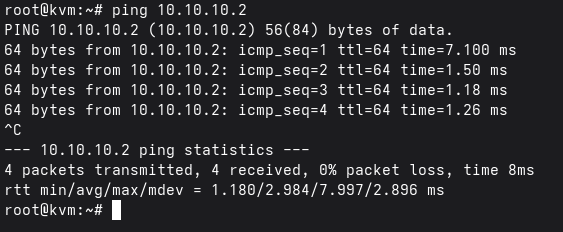
\includegraphics[width=\textwidth,keepaspectratio]{figures/tests/server1_to_server2_management.png}
    \caption{Ping test: Server~1 $\rightarrow$ Server~2 (management, 10.10.10.2).}
    \label{fig:app-test-s1-s2-mgmt}
\end{figure}

\begin{figure}[H]
    \centering
    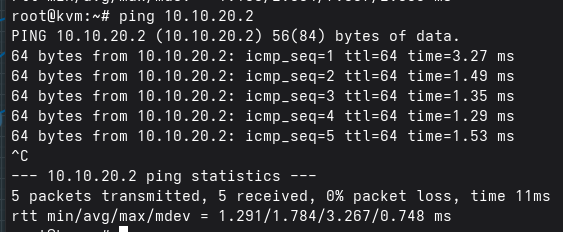
\includegraphics[width=\textwidth,keepaspectratio]{figures/tests/server1_to_server2_service.png}
    \caption{Ping test: Server~1 $\rightarrow$ Server~2 (service, 10.10.20.2).}
    \label{fig:app-test-s1-s2-svc}
\end{figure}

\section{Intra-zone connectivity tests}
\addcontentsline{toc}{section}{D.2 Intra-zone connectivity tests}

\begin{figure}[H]
    \centering
    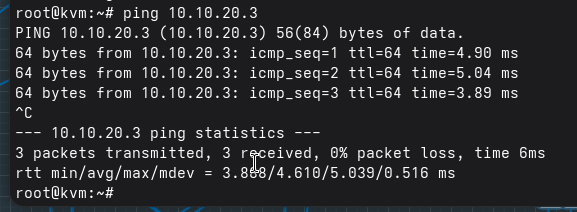
\includegraphics[width=\textwidth,keepaspectratio]{figures/tests/server1_to_server3_service.png}
    \caption{Ping test: Server~1 $\rightarrow$ Server~3 (service, 10.10.20.3).}
    \label{fig:app-test-s1-s3-svc}
\end{figure}

\begin{figure}[H]
    \centering
    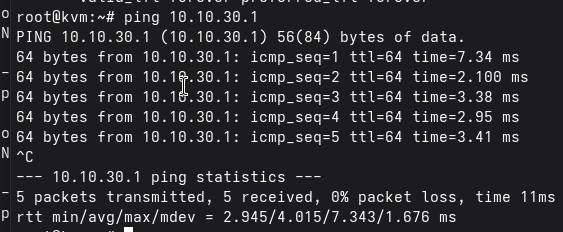
\includegraphics[width=\textwidth,keepaspectratio]{figures/tests/server1_to_server5_service.png}
    \caption{Ping test: Server~1 $\rightarrow$ Server~5 (service, 10.10.30.1).}
    \label{fig:app-test-s1-s5-svc}
\end{figure}

\begin{figure}[H]
    \centering
    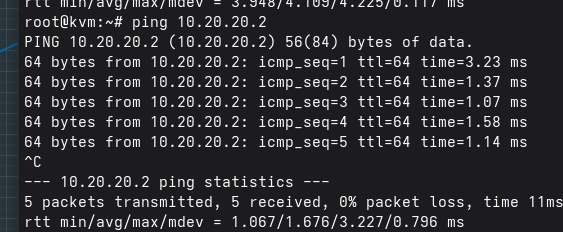
\includegraphics[width=\textwidth,keepaspectratio]{figures/tests/server7_to_server8_service.png}
    \caption{Ping test: Server~7 $\rightarrow$ Server~8 (service, 10.20.20.2).}
    \label{fig:app-test-s7-s8-svc}
\end{figure}

\section{Inter-zone security tests}
\addcontentsline{toc}{section}{D.3 Inter-zone security tests}

\begin{figure}[H]
    \centering
    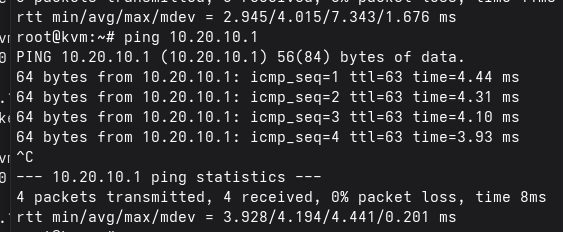
\includegraphics[width=\textwidth,keepaspectratio]{figures/tests/server1_to_server7_management.png}
    \caption{Ping test: Server~1 $\rightarrow$ Server~7 (management, 10.20.10.1), permitted.}
    \label{fig:app-test-s1-s7-mgmt}
\end{figure}

\begin{figure}[H]
    \centering
    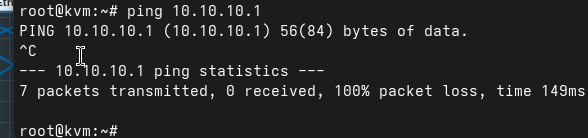
\includegraphics[width=\textwidth,keepaspectratio]{figures/tests/server7_to_server1_management(blocked).png}
    \caption{Ping test: Server~7 $\rightarrow$ Server~1 (management, 10.10.10.1), blocked.}
    \label{fig:app-test-s7-s1-mgmt-block}
\end{figure}

\chapter{Appendix E: Configuration Verification Screenshots}
\label{app:config-verify}

\section{EoR-1 (Arista vEOS)}
\addcontentsline{toc}{section}{E.1 EoR-1}

\begin{figure}[H]
    \centering
    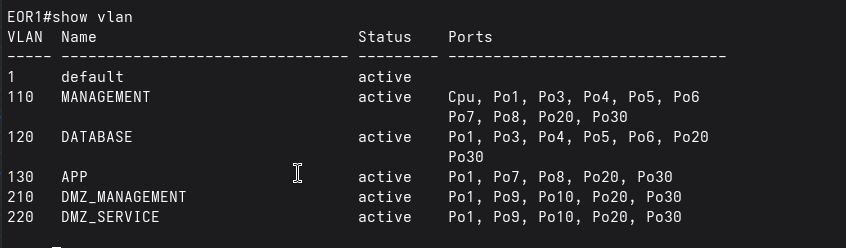
\includegraphics[width=\textwidth,keepaspectratio]{figures/eor1/eor1_vlans.png}
    \caption{EoR-1: VLANs (\texttt{show vlan}).}
    \label{fig:app-eor1-vlans}
\end{figure}

\begin{figure}[H]
    \centering
    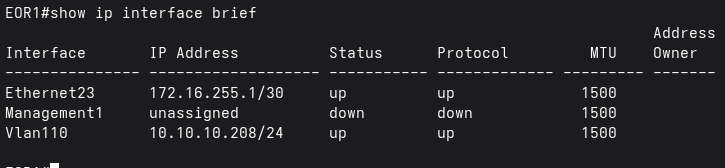
\includegraphics[width=\textwidth,keepaspectratio]{figures/eor1/eor1_ip.png}
    \caption{EoR-1: IP addressing (\texttt{show ip interface brief}).}
    \label{fig:app-eor1-ip}
\end{figure}

\begin{figure}[H]
    \centering
    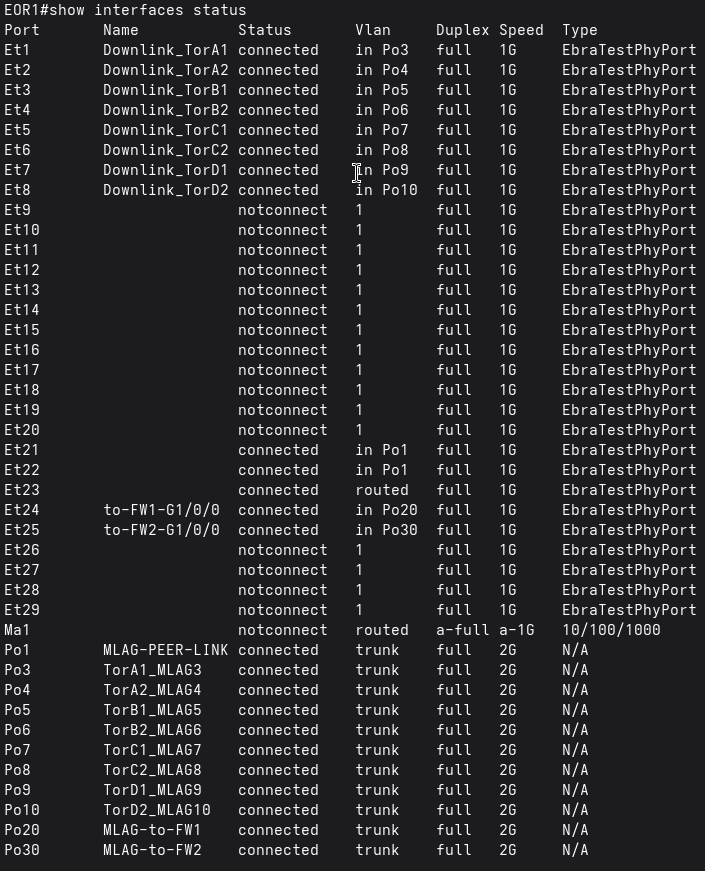
\includegraphics[width=\textwidth,keepaspectratio]{figures/eor1/eor1_interfaces.png}
    \caption{EoR-1: Interfaces and Port-Channels.}
    \label{fig:app-eor1-interfaces}
\end{figure}

\begin{figure}[H]
    \centering
    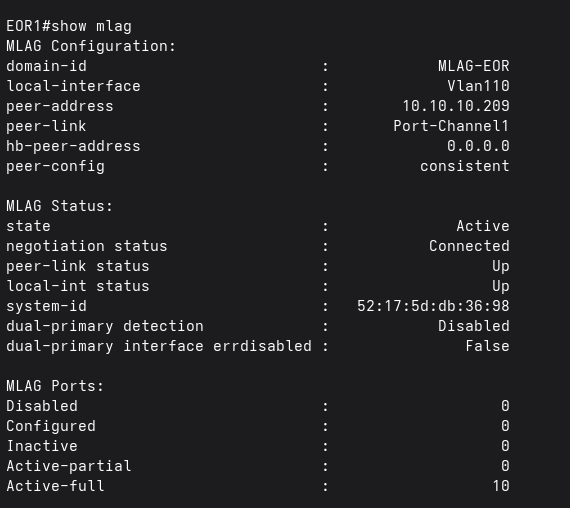
\includegraphics[width=\textwidth,keepaspectratio]{figures/eor1/eor1_mlag_default.png}
    \caption{EoR-1: MLAG (\texttt{show mlag}).}
    \label{fig:app-eor1-mlag}
\end{figure}

\section{ToR A-1 (Arista vEOS)}
\addcontentsline{toc}{section}{E.2 ToR A-1}

\begin{figure}[H]
    \centering
    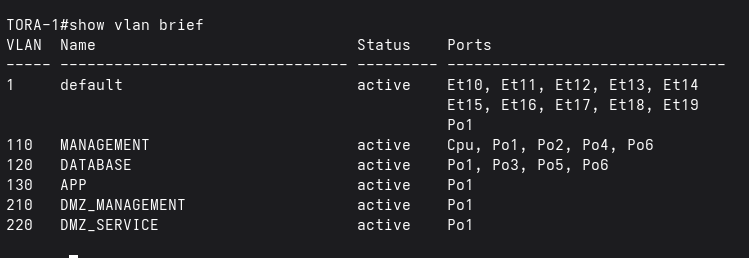
\includegraphics[width=\textwidth,keepaspectratio]{figures/tora1/tora1_vlan.png}
    \caption{ToR A-1: VLANs (\texttt{show vlan brief}).}
    \label{fig:app-tora1-vlans}
\end{figure}

\begin{figure}[H]
    \centering
    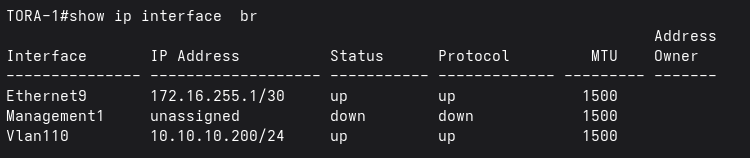
\includegraphics[width=\textwidth,keepaspectratio]{figures/tora1/tora1_ip.png}
    \caption{ToR A-1: IP addressing.}
    \label{fig:app-tora1-ip}
\end{figure}

\begin{figure}[H]
    \centering
    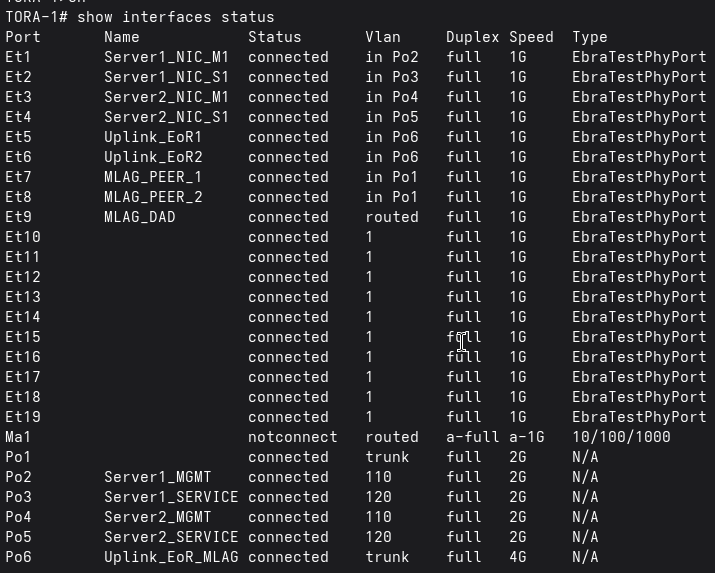
\includegraphics[width=\textwidth,keepaspectratio]{figures/tora1/tora1_interfaces.png}
    \caption{ToR A-1: Interfaces and Port-Channels.}
    \label{fig:app-tora1-interfaces}
\end{figure}

\begin{figure}[H]
    \centering
    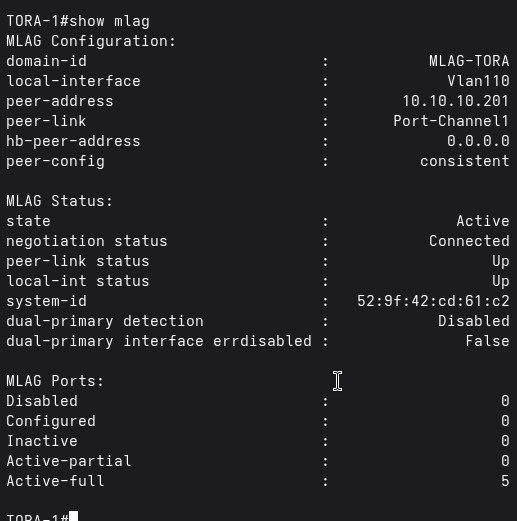
\includegraphics[width=\textwidth,keepaspectratio]{figures/tora1/tora1_mlag_default.png}
    \caption{ToR A-1: MLAG (\texttt{show mlag}).}
    \label{fig:app-tora1-mlag}
\end{figure}

\section{Firewalls (pfSense)}
\addcontentsline{toc}{section}{E.3 Firewalls}

\begin{figure}[H]
    \centering
    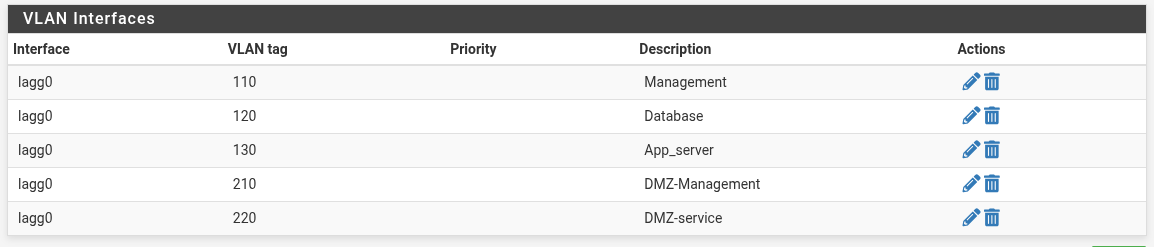
\includegraphics[width=\textwidth,keepaspectratio]{figures/fw1/fw1_vlan.png}
    \caption{FW-1: VLAN interfaces.}
    \label{fig:app-fw1-vlans}
\end{figure}

\begin{figure}[H]
    \centering
    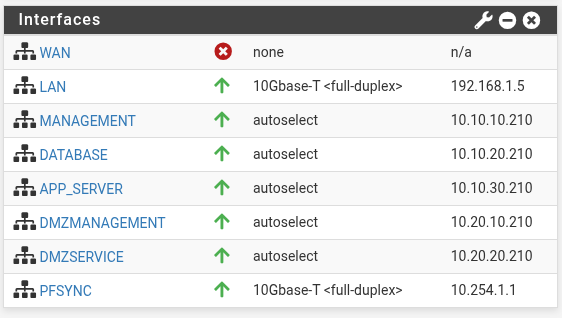
\includegraphics[width=\textwidth,keepaspectratio]{figures/fw1/fw1_interfaces_ips.png}
    \caption{FW-1: Interfaces and IPs.}
    \label{fig:app-fw1-interfaces}
\end{figure}

\begin{figure}[H]
    \centering
    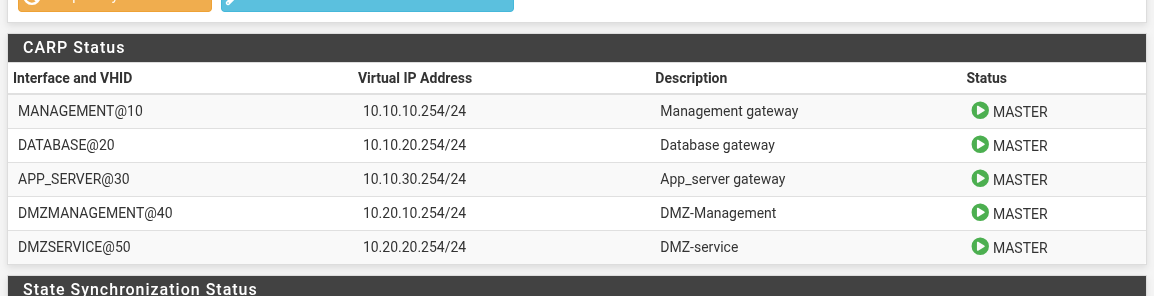
\includegraphics[width=\textwidth,keepaspectratio]{figures/fw1/fw1_vrrp.png}
    \caption{FW-1: CARP (master).}
    \label{fig:app-fw1-vrrp}
\end{figure}

\begin{figure}[H]
    \centering
    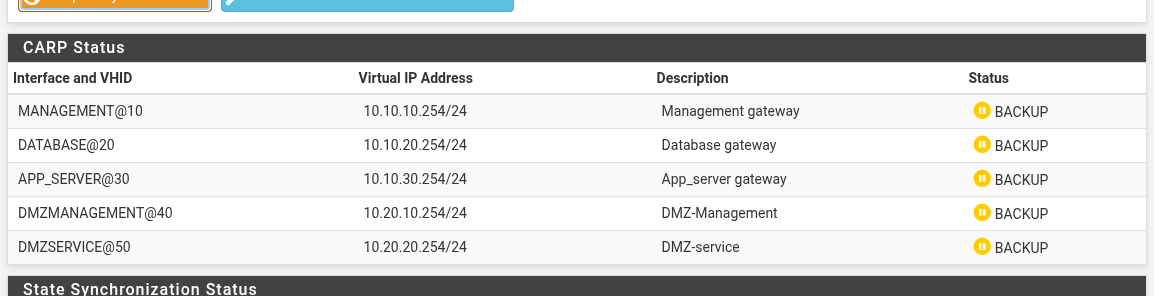
\includegraphics[width=\textwidth,keepaspectratio]{figures/fw1/fw2_vrrp.png}
    \caption{FW-2: CARP (backup).}
    \label{fig:app-fw2-vrrp}
\end{figure}

\begin{figure}[H]
    \centering
    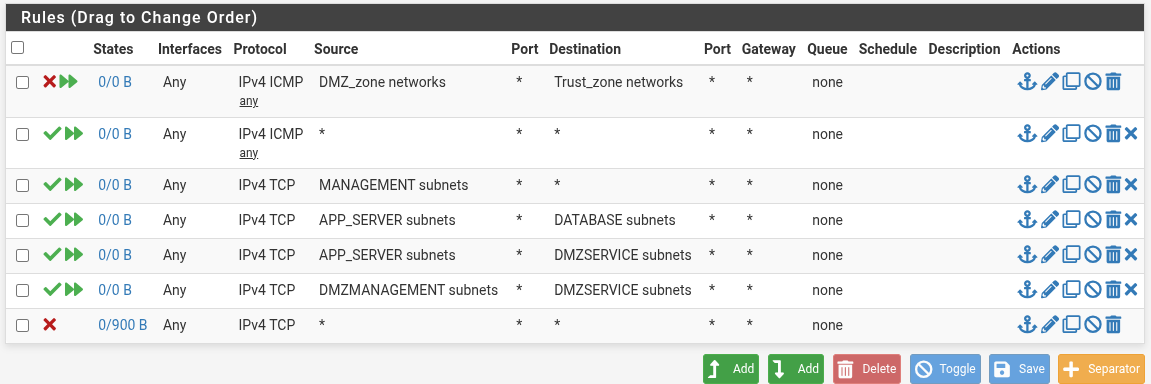
\includegraphics[width=\textwidth,keepaspectratio]{figures/fw1/fw1_rules.png}
    \caption{FW-1: Firewall rules.}
    \label{fig:app-fw1-rules}
\end{figure}

\section{Server 1 (Linux)}
\addcontentsline{toc}{section}{E.4 Server 1}

\begin{figure}[H]
    \centering
    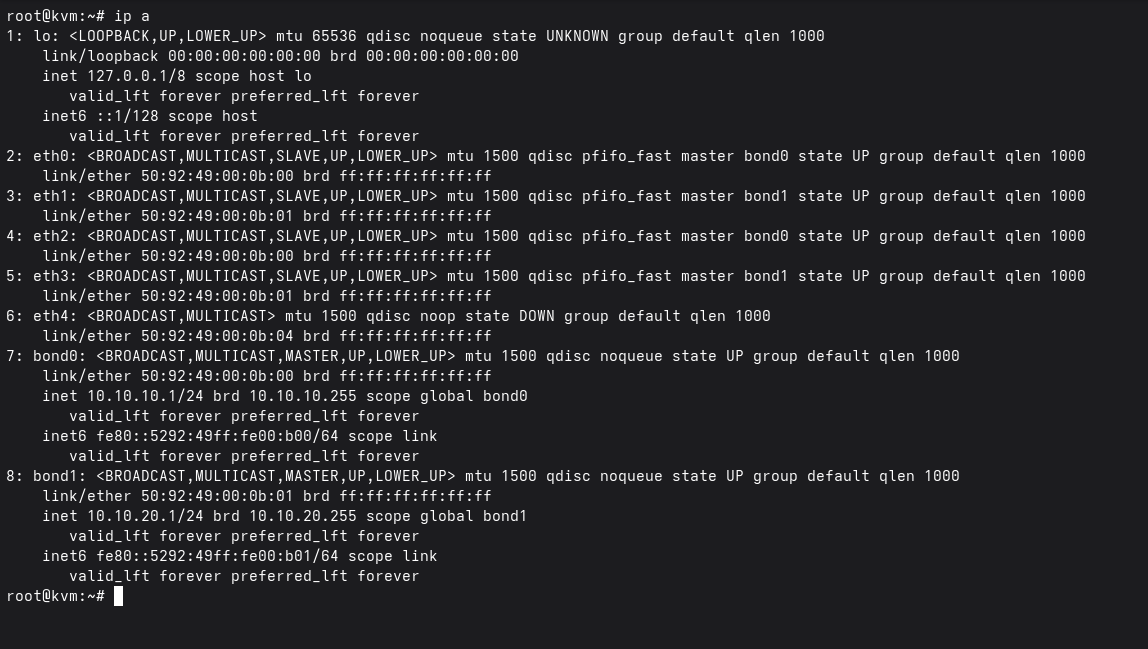
\includegraphics[width=\textwidth,keepaspectratio]{figures/server1/server1_config.png}
    \caption{Server~1: Bonding and IP assignments (\texttt{ip a}).}
    \label{fig:app-server1-config}
\end{figure}


% ===== BIBLIOGRAPHY (at the very end) =====
\clearpage
\bibliographystyle{unsrtnat}
\renewcommand{\bibname}{Bibliography}
\addcontentsline{toc}{chapter}{Bibliography}
\bibliography{references}
\chapter*{Abstract}
\addcontentsline{toc}{chapter}{Abstract}

\begingroup
\small
\linespread{1.05}\selectfont
\setlength{\parskip}{0.3em}

This dissertation, prepared for the Licence degree in ISIL at USTHB, presents the design and simulation of a modern data center network architecture suited to highly available enterprise workloads. The project adopts a spine-leaf topology with full-mesh connectivity between eight Top-of-Rack leaf switches and two End-of-Rack spine switches, complemented by zone-based security at the network edge. The infrastructure is realized in a virtual laboratory: PNETLab emulates the switching and firewall fabric, while VMware Workstation hosts Linux servers distributed across four cabinets.

The proposed facility organizes four cabinets into distinct roles and security zones. Cabinets A, B, and C form the Trust zone, hosting database and application servers; Cabinet D hosts web-facing services in the DMZ. Two perimeter firewalls operate in an active-standby cluster using CARP, enforcing strict separation so that external or DMZ compromise cannot reach internal databases without explicit policy. Each of the eight servers connects through dual management and service network interfaces, bonded for resilience and mapped to dedicated VLANs for management (110, 210), database (120), application (130), and web (220) traffic. At every layer (firewall, spine, and leaf), redundancy eliminates single points of failure: MLAG pairs at ToR and EoR and VRRP/CARP gateways.

The design is specified through functional and non-functional requirements, actor responsibilities, UML use-case and sequence models, a high-level topology, and low-level documentation including device inventory, IP addressing, and port-level cabling matrices. The implementation stack combines PNETLab, VMware Workstation Pro, Arista vEOS switches, pfSense firewalls, and Debian servers. Switches were configured with VLANs, trunk and access Port-Channels, MLAG domains, and management SVIs; firewalls with zone-based rules and default-deny policies; servers with active-backup bonding on management and service planes.

End-to-end validation combined connectivity testing and deliberate failure injection. ICMP tests confirmed allowed flows within and across cabinets on both management and service networks, as well as blocked DMZ-to-Trust management paths where policy required denial. Shutting down active firewalls, spine switches, and leaf switches demonstrated sub-second failover to standby nodes without loss of forwarding. Together, these results confirm that the architecture meets its redundancy, security, and manageability objectives.

The outcome is a coherent, fully documented, and rigorously tested blueprint, from topology and addressing through configuration templates and test evidence, that translates modern spine-leaf and zero-trust zoning principles into a production-ready enterprise data center design.

\endgroup


\end{document}
